\documentclass[11pt,a4paper,fontset=windows,UTF8]{ctexart}
% !TEX program = xelatex
% 数译体例 · 中文数学译注本 通用导言
\usepackage{amsmath,amssymb,amsthm,mathtools,mathrsfs}
\usepackage[margin=2.6cm,footskip=1.1cm]{geometry}
\usepackage{graphicx}
\usepackage{float}
\graphicspath{{figures/}{../figures/}}
\usepackage{booktabs,array,longtable}
\usepackage{enumitem}
\usepackage{xcolor}
\usepackage{fancyhdr}
\usepackage{tikz}
\usepackage[hidelinks,bookmarksnumbered]{hyperref}
\usepackage{xurl}

% --- 字体与版式（ctexart 已在文档类中设置 fontset=windows）---
\linespread{1.15}
\setlength{\parskip}{0.15em}
\setlength{\emergencystretch}{3em}
\hbadness=10000
\setlist{itemsep=0.15em,topsep=0.3em,leftmargin=2em}

% --- 语义宏：范畴与算子 ---
\newcommand{\cat}[1]{\mathcal{#1}}
\newcommand{\Bun}{\operatorname{Bun}}
\newcommand{\Loc}{\operatorname{Loc}}
\newcommand{\QCoh}{\operatorname{QCoh}}
\newcommand{\IndCoh}{\operatorname{IndCoh}}
\newcommand{\Shv}{\operatorname{Shv}}
\newcommand{\Rep}{\operatorname{Rep}}
\newcommand{\Sph}{\operatorname{Sph}}
\newcommand{\Gr}{\operatorname{Gr}}
\newcommand{\Higgs}{\operatorname{Higgs}}
\newcommand{\Hitch}{\operatorname{Hitch}}
\newcommand{\Nilp}{\operatorname{Nilp}}
\newcommand{\Op}{\operatorname{Op}}
\newcommand{\Dmod}{\mathcal{D}\text{-}\mathrm{mod}}
\newcommand{\Gd}{\check{G}}
\newcommand{\gd}{\check{\mathfrak{g}}}
\newcommand{\C}{\mathbb{C}}
\newcommand{\R}{\mathbb{R}}
\newcommand{\Z}{\mathbb{Z}}
\newcommand{\Q}{\mathbb{Q}}
\newcommand{\F}{\mathbb{F}}
\newcommand{\PP}{\mathbb{P}}
\newcommand{\A}{\mathbb{A}}
\newcommand{\OO}{\mathcal{O}}
\newcommand{\LG}{\mathcal{L}G}
\newcommand{\LGp}{\mathcal{L}^{+}G}
\newcommand{\fr}[1]{\mathfrak{#1}}
\newcommand{\dR}{\mathrm{dR}}
\newcommand{\Betti}{\mathrm{Betti}}
\newcommand{\et}{\mathrm{\acute{e}t}}
\newcommand{\id}{\mathrm{id}}
\newcommand{\pt}{\mathrm{pt}}
\newcommand{\triv}{\mathrm{triv}}

% --- 译注：正文用脚注，附录由脚本汇总 ---
\newcommand{\zhnote}[1]{\footnote{译注｜#1}}
% 术语首次出现：中文（English, 缩写）
\newcommand{\term}[3]{#1（#2#3）}

% --- 定理环境 ---
\theoremstyle{plain}
\newtheorem{theorem}{定理}
\newtheorem*{theorem*}{定理}
\newtheorem*{conjecture*}{猜想}
\theoremstyle{definition}
\newtheorem*{remark*}{注}
\newtheorem*{definition*}{定义}
\newtheorem*{example*}{例}

% --- 页眉页脚 ---
\pagestyle{fancy}
\fancyhf{}
\fancyhead[L]{\small 几何朗兰兹对偶是什么？}
\fancyhead[R]{\small David Ben-Zvi}
\fancyfoot[C]{\small\thepage}
\renewcommand{\headrulewidth}{0.3pt}

% --- 题注 ---
\usepackage{caption}
\captionsetup{font=small,labelfont=bf}


\newcommand{\anote}[1]{\footnote{原注｜#1}}

\begin{document}

% ===================== 标题页 =====================
\begin{titlepage}
\centering
\vspace*{2.2cm}
{\Huge\bfseries 几何朗兰兹对偶\\[6pt]是什么？\par}
\vspace{0.8cm}
{\Large What is the Geometric Langlands\\[4pt]Correspondence About?\par}
\vspace{1.6cm}
{\large David Ben-Zvi\par}
\vspace{0.2cm}
{\normalsize（德克萨斯大学奥斯汀分校数学系）\par}
\vspace{1.2cm}
{\large 插图：Elliot Kienzle\par}
\vspace{1.6cm}
{\large 中文译注本\par}
\vspace{0.3cm}
{\normalsize 译者：数译工程\par}
\vspace{0.3cm}
{\normalsize 底本：arXiv:2605.23167v1 [math.RT]，2026 年 5 月 22 日\par}
\vfill
{\small 2026 年 11 月\par}
\end{titlepage}

% ===================== 译者说明 =====================
\section*{译者说明}
\addcontentsline{toc}{section}{译者说明}

\paragraph{底本。}本译本依据 David Ben-Zvi 的综述 \emph{What is the Geometric Langlands Correspondence About?}（arXiv:2605.23167v1，math.RT，2026 年 5 月 22 日；作者自注收稿日期为 2026 年 5 月 25 日）。原文是面向一般数学读者的导论性文章，正文约三十页，参考文献一百二十余条。译文按原文章节顺序逐段移译，公式编号沿用原编号体系，节号与原文章节号一致，便于对照阅读。

\paragraph{体例。}专业术语首次出现时给出“中文（English）”形式，其后统一使用中文或已约定俗成的缩写；原文以斜体标出的书名、刊名与拉丁术语，译文保留原文。人名、群名、定理名（Hecke、Hitchin、Langlands、Satake、Whittaker 等）一律不音译，直接保留拉丁拼写。正文只放译文；凡译者所加的补白、出处与辨析，一律入脚注，以“译注｜”起首，与作者的“原注｜”相区别。每一条解释性译注都标注来源等级：
\begin{itemize}
\item \textbf{A 级}：原始文献（作者原文、原始论文、权威工具书）；
\item \textbf{B 级}：权威综述与百科（nLab、Stacks Project、MathWorld、EMS 等）；
\item \textbf{I 级}：译者依据上下文所作的推断（标“译者按（无外部依据）”）。
\end{itemize}

\paragraph{nLab 批注。}应委托要求，本译本以 nLab 词条为主要参考资料，对文中的核心概念逐处加注。这类批注有两种作用：一是核对术语与定义的精确含义（例如“自守层”与“Hecke 本征层”的关系、“谱侧”范畴 $\IndCoh_{\Nilp}(\Loc_{\Gd})$ 中下标的来历），二是把原文一笔带过、读者却可能卡住的结构补足（例如几何 Satake 等价为何能“从无到有”造出对偶群、因子化为何是交换性的来源）。批注中的 nLab 链接均为 2026 年 11 月可访问的版本；nLab 是维基式词条，内容会持续修订，读者若发现与今本不符，应以词条当前版本为准。文末附“译注汇总”，逐条重列全部译注并标明所在节，便于不翻正文而通读批注。

\paragraph{符号。}全文固定使用下列记号：$G$ 为 $\C$ 上连通约化群，$\Gd$ 为其朗兰兹对偶群；$C$ 为 $\C$ 上光滑射影曲线（等价地，紧黎曼面）；$\Bun_{G}$ 为 $C$ 上 $G$-丛的模栈；$\Loc_{\Gd}$ 为 $\Gd$-局部系统的模栈（“特征簇”的整体版本）；$\Shv(X)$ 泛指 $X$ 上某一套六函子形式下的层范畴，$\Dmod(X)$ 为 D-模范畴，$\QCoh(X)$、$\IndCoh(X)$ 分别为拟凝聚层与归纳凝聚层范畴；$\Sph_{G}=\Shv(\Gr_{G})^{\LGp}$ 为球 Hecke 范畴，$\Gr_{G}=\LG/\LGp$ 为仿射 Grassmannian；$\fr{g}=\operatorname{Lie}G$。原文以 $\mathcal{H}$ 记希尔伯特空间、以 $H$ 记算子，译文照此区分。

\paragraph{致谢与责任。}译文力求贴合作者原意；凡因译者理解偏差而生的错误，由译者负责，并欢迎指正。原文三幅插图由 Elliot Kienzle 绘制，本译本直接取自 arXiv 预印本内嵌的原图，仅作学术阅读之说明性使用。

\clearpage

% ===================== 摘要 =====================
\section*{摘要}
\addcontentsline{toc}{section}{摘要}

最近，非分歧几何朗兰兹猜想的证明引起了广泛关注，因此现在似乎是回答标题之问的好时机。用一句话说，几何朗兰兹对偶是关于某一类称为\emph{自守层}（automorphic sheaf）的微分方程的代数谱定理：它断言，这些对象可以分解为“单色”的构件，而这些构件把自然对称性（Hecke 算子）的作用对角化；它同时刻画了相应的“颜色”或“频率”，即 Langlands 参数。

这个陈述听起来极为技术化且玄奥，其证明长达数千页，而可以直接陈述的即时推论相对很少。那么它究竟是怎么回事？在这篇简短综述中，我将以非正式的方式把这一主题呈现为“非阿贝尔对称性研究总蓝图”，并触及一些主要的动机、联系与已经浮现的结构。

\medskip
\noindent\textit{本文的配套视频见} \url{https://www.youtube.com/watch?v=yxauvlBZCAU}。

\clearpage
\tableofcontents
\clearpage

\section*{引言}\label{sec:0}
\addcontentsline{toc}{section}{引言}

谱定理与傅里叶变换在数学与物理中无处不在。就其根本而言，它们关乎如何利用阿贝尔对称性（例如空间平移）把函数分解为简单、单色的构件。人们自然会想：非阿贝尔对称性的对应物想必更为强大、也更为有用。然而，我们今天对非阿贝尔对偶的理解，仍不免让人想起“盲人摸象”的寓言。数论学家已经为这种非阿贝尔对偶发现了一幅宏大图景——朗兰兹纲领，其回声遍及表示论，应用众多（其中最著名者即费马大定理的证明）。物理学家则独立地给出了另一幅宏大图景：麦克斯韦（Maxwell）理论中电磁对偶的非阿贝尔形式，即所谓 Montonen--Olive S-对偶，其回声同样遍及数学物理。得益于对几何朗兰兹对偶（Geometric Langlands Correspondence，以下简称 GLC）的研究，我们现在明白：这两个群体实际上是在勘察同一头巨象，而且如今已能交换观察、协调彼此的考察。事实上，我们或许已经辨认出这头巨兽跳动的心脏——由因子化代数（factorization algebra）这一概念所提供的、隐藏的交换性。

这一探索近来迎来了一个重大里程碑：Gaitsgory 与 Raskin 会同 Arinkin、Beraldo、\mbox{Campbell}、Chen、Faergeman、Lin 与 Rozenblyum，证明了非分歧几何朗兰兹猜想。该证明展开为三篇论文 [GR24a, ABC${}^{+}$24a, GR24b] 与一部两卷本专著 [ABC${}^{+}$24b, CCF${}^{+}$24]，其基础是此前的大量技术工作，包括 Lurie 关于高阶代数的基础 [Lur09, Lur]，以及 Gaitsgory 过去二十年间的许多工作。要理解 GLC 的陈述——更不必说其证明——须得穿透一层又一层的坚韧厚皮，并在众多活动部件之间穿行。但我相信，由此获得的洞见与视角足以回报这番努力，并且指向一个远比眼前所见更为宏大的整体。

我想借此机会作一番综述：GLC 究竟是怎样一种陈述，我们为何应当关心它，以及它为何成立。这绝不是一份关于证明的详尽叙述。我的重点放在那些最令我着迷的部分——它的众多联系与视角，以及它帮助揭示的深层结构。我先在 \S\ref{sec:1} 中讨论谱定理与傅里叶变换，以此铺开整个故事；接着在 \S\ref{sec:2} 中给出 GLC 的具体背景（陈述最终落在 \S\ref{sec:2.5}）。\S\ref{sec:3} 与 \S\ref{sec:4} 讨论两个主要结构——因子化与 Hitchin 系统——它们提示 GLC 可能为真；随后在 \S\ref{sec:5} 中概述证明。最后在 \S\ref{sec:6} 中谈一些应用——急于知道我们忙这一切究竟为了什么的读者，不妨先翻到这里——以及接下来可能的方向。

\textit{Caveat lector}（读者须知）：我始终宁可偏向直觉而牺牲精确，宁可引用综述文章而不引原始文献。在引用相关论文与重要进展方面，我远谈不上全面，甚至算不上合格。我也没有讨论 GLC 宇宙的“第一阶段”（Phase I）——从问题在 [Dri83, Lau87] 中的起源，到 [FGV01, Gai04] 中 $\mathrm{GL}_{n}$ 的 Hecke 本征层的构造（该领域早期的综述见 [Fre04, Gai17a]）——而是聚焦于第二阶段（Phase II）的精华，即范畴化的 GLC（categorical GLC），从 [BD] 直到其最近的证明。\zhnote{“第一阶段／第二阶段”（Phase I / Phase II）是作者本人对几何朗兰兹发展史的分期，本译本照原文保留：Phase I 自问题的提出（[Dri83, Lau87]）延伸到 $\mathrm{GL}_{n}$ 的 Hecke 本征层之构造（[FGV01, Gai04]），其综述见 [Fre04, Gai17a]；Phase II 即“范畴化的 GLC”，以 [BD] 为起点，经 Arinkin--Gaitsgory 引入奇异支撑与 $\IndCoh_{\Nilp}$ 的表述（[AG15]），直至 2024 年非分歧猜想的证明（[GR24a, GR24b, ABC${}^{+}$24a, ABC${}^{+}$24b, CCF${}^{+}$24]）。原文所谓 “the greatest hits of Phase II” 即指这一时期的代表性成果。[来源：A 级，Ben-Zvi 原文所述分期；[BD]、[AG15] 与 [Sch26] 互证]}我热忱推荐 [Sch26]，那是对几何朗兰兹纲领现状一份富有洞见、深入详尽的叙述。

\textit{致谢}：感谢“当前进展通报”（Current Events Bulletin）的组织者 Daniel Erman 与 Bianca Viray。\zhnote{\emph{Current Events Bulletin}（“当前进展通报”）是美国数学会在年度联合数学会议（Joint Mathematics Meetings）上组织的综述报告系列，本文的致谢对象即该系列的当届组织者。[来源：B 级，AMS 会议页面 \url{https://www.ams.org/meetings/lectures/current-events-bulletin}]}同样感谢 Alexandre Afgoustidis、Ron Donagi、Nigel Higson、Masoud Kamgarpour、JiWoong Park 与 Sam Raskin 对早期稿本提出的宝贵意见。本研究得到美国国家科学基金会（National Science Foundation）DMS-2302356 号资助，谨致谢意。

\section{这是怎样一种陈述？}\label{sec:1}

我将把几何朗兰兹对偶描述为谱定理（spectral theorem）的非阿贝尔对应物。为此，我们先回头重温谱定理。

\subsection{谱定理}\label{sec:1.1}

谱定理为希尔伯特空间 $\mathcal{H}$ 上的自伴算子（self-adjoint operator）$H$ 提供了一套谱分解理论。它为我们熟知的事实——实对称矩阵，或更一般地，复埃尔米特矩阵可以对角化——提供了普遍背景。该事实可以解释为：底层的希尔伯特空间 $\mathcal{H}\cong\C^{n}$ 分解为本征空间（eigenspace）的直和
\begin{equation}\label{eq:1.1}
\mathcal{H}\;\cong\;\bigoplus_{\lambda\in\R_{t}}\mathcal{H}_{\lambda}.
\end{equation}
我们可以把每个 $\mathcal{H}_{\lambda}$ 看作“生活在”相应的点 $\lambda\in\R_{t}$ 之上，于是对 $\R_{t}$ 的任意子集，都可把相应本征空间之和定义为与之对应的子空间。（这里 $\R_{t}$ 表示带坐标 $t$ 的一份 $\R$ 的拷贝，这是我们用来记本征值与谱测度之定义域的记号，即动量空间。）利用这一描述，$\R_{t}$ 上的一切函数都通过“在谱上取值”而成为 $\mathcal{H}$ 上彼此交换的算子（$f$ 在 $\mathcal{H}_{\lambda}$ 上乘以 $f(\lambda)$），从而 $H$ 的作用就是乘以坐标函数 $t$——这就是泛函演算（functional calculus）。

对一般的（可能无界的）自伴算子，$\mathcal{H}$ 中未必真有本征向量；谱定理借助测度论给出一种意义，使 $\mathcal{H}$ 中所有向量都可以写成以 $\lambda\in\R_{t}$ 为本征值的本征向量的连续线性组合——即在 $\R_{t}$ 上的积分；实际上，这把 $\mathcal{H}$ 铺展成 $\R_{t}$ 上的一族向量空间。这可以用 $\mathcal{H}$ 上的投影值测度（projection-valued measure）表述，也可以更抽象地用 $\R_{t}$ 上可测的希尔伯特空间族表述。这相当于在 $\R_{t}$ 上定义一个取值于希尔伯特空间的测度 $d\mathcal{H}(t)$，使得希尔伯特空间 $\mathcal{H}$ 连同算子 $H$ 可以作为直积分（direct integral，或“整体截面”）复原：
\begin{equation}\label{eq:1.2}
\mathcal{H}\;=\;\int^{\oplus}_{\R_{t}} d\mathcal{H}(t),
\end{equation}
而在区间 $I\subset\R_{t}$ 上的积分给出子空间 $\mathcal{H}_{I}\subset\mathcal{H}$，$H$ 的谱落在 $I$ 中。在这一描述里，算子 $H$ 由坐标函数 $t$ 的作用给出。该作用可延拓为 Borel 泛函演算：所有 Borel 可测函数都以彼此交换的（可能无界的）算子作用于 $\R_{t}$——例如区间 $I$ 的示性函数投影到 $\mathcal{H}_{I}$ 上。变体包括连续泛函演算（使 $\mathcal{H}$ 成为交换 $C^{*}$-代数 $C_{c}(\R_{t})$ 上的模）与有界泛函演算（使 $\mathcal{H}$ 成为交换 von Neumann 代数 $L^{\infty}(\R_{t})$ 上的模）。

对二元组 $(\mathcal{H},H)$ 还有一种“取指数”的观点（同样来自泛函演算）：它定义了群 $\R_{x}$ 在 $\mathcal{H}$ 上的酉表示 $x\mapsto e^{ixH}$（$\R_{x}$ 是 $\R$ 的对偶拷贝，带坐标 $x$，即位置空间）。从这个角度看，谱定理完整刻画了 $\R_{x}$ 的酉表示，把它们拆成“原子”部件——不可约酉表示，即一维本征空间 $\C_{\lambda}$。谱定理就这样为描述其他群的表示论提供了蓝图。

然而，配备自伴算子或配备 $\R_{x}$ 酉表示的希尔伯特空间是活生生的对象，它们并不只是构成一个集合：它们有内部对称性，并且可以通过与作用交换的有界线性算子（例如酉算子）彼此“交谈”。换言之，它们构成一个范畴；实际上（经由泛函演算）是一个算子代数上的模范畴。虽然通常不这样表述，谱定理可以升级为范畴等价
\[
\{\text{带自伴算子的希尔伯特空间}\}\;\longleftrightarrow\;\{\R_{t}\ \text{上可测的希尔伯特空间族}\}.
\]
也就是说，我们不仅能对对象、也能对态射作谱分解，把态射分解为多重度空间之间的线性算子。这同样是一个模型，告诉我们该如何去描述别的表示论。\zhnote{把谱定理读作“表示范畴与谱侧范畴的等价”，实质上是 Tannaka 对偶（Tannaka duality）在交换群 $\R$ 上的特例：由表示范畴连同遗忘函子可以重构出群，而谱侧正是“所有颜色／参数”的栖身之处。参见 nLab 词条 \emph{Tannaka duality}，\href{https://ncatlab.org/nlab/show/Tannaka+duality}{\texttt{https:/\allowbreak{}/\allowbreak{}ncatlab.\allowbreak{}org/\allowbreak{}nlab/\allowbreak{}show/\allowbreak{}Tannaka+\allowbreak{}duality}}（最后修订 2025-07-28）。这也预示了几何朗兰兹对偶的基本形状：一侧是范畴，另一侧是其“谱”。}

\subsection{谱定理与傅里叶变换}\label{sec:1.2}

谱定理与傅里叶变换（Fourier transform）之间有一种共生关系。一方面，傅里叶变换
\[
L^{2}(\R_{x})\overset{\sim}{\longrightarrow}L^{2}(\R_{t}),\qquad
\hat{f}(t)=\int_{\R}f(x)e^{-2\pi ixt}\,dx
\]
可以说其根本特征就在于：它把 $x$ 中的平移、微分与卷积算子变成 $t$ 中的乘法算子——也就是同时把群 $\R$（一个酉表示）、它的李代数（一个自伴算子）与它的群代数（一个算子代数）的作用对角化。用谱定理的语言说，傅里叶变换断言：正则表示 $\R_{x}\curvearrowright L^{2}(\R_{x})$（等价地，算子 $i\frac{d}{dx}$）的谱分解由 $L^{2}(\R_{t})=\int^{\oplus}_{\R_{t}}\C_{t}\,dt$ 给出，即 $\R_{t}$ 上“常秩一”的希尔伯特空间族，每个频率的重数都是一。换个说法，傅里叶反演
\begin{equation}\label{eq:1.3}
f(x)=\int_{\R}\hat{f}(t)e^{2\pi ixt}\,dt
\end{equation}
让我们把函数构造为指数函数的叠加；这些指数函数是平移的本征函数，也就是由频率（颜色）$t$ 参数化的纯频率（单色）波。

另一方面，谱定理本身也可以看作一种“范畴化”的傅里叶变换：其中复值函数或测度及其积分 \eqref{eq:1.3} 被取值于向量空间的测度及其直积分 \eqref{eq:1.2} 取代。在这一类比中，经傅里叶变换变成 $\delta$-函数 $\delta_{\lambda}$ 的单色波 $e^{i\lambda x}$，被 $\R_{x}$ 的不可约表示取代，即抽象的本征空间 $\C_{\lambda}$；谱分解把它们变成 $\lambda\in\R_{t}$ 处的“摩天楼”（取值于向量空间的 $\delta$-函数）$\C_{\lambda}$。谱定理于是让我们把任意酉表示写成由其本征空间给出的向量空间值函数的直积分（叠加）。正则表示 $L^{2}(\R_{x})$ 扮演“白光”的角色——所有可能频率的叠加；它的变换 $L^{2}(\R_{t})$ 确实处处支撑在 $t$ 轴上。

我们把这一类比的要点总结在下表中：

\begin{center}
\renewcommand{\arraystretch}{1.25}
\begin{tabular}{ll}
\toprule
傅里叶变换 & 谱定理\\
\midrule
$e^{i\lambda x}$ & $\C_{\lambda}$\\
$f(x)$ & $(\mathcal{H},H)$\\
指数函数的积分 & 本征空间的直积分\\
数 & 向量空间\\
希尔伯特空间 $L^{2}(\R)$ & 酉表示的范畴\\
\bottomrule
\end{tabular}
\end{center}

这一看待谱定理的视角也许显得想入非非，但它其实极其有用。具体说来，把谱定理视为傅里叶变换的变体，提示了刻画并进而证明它们的强有力途径——我们在几何朗兰兹对偶的情形中将会看到这一点。

\subsection{很好，但几何朗兰兹在哪里？}\label{sec:1.3}

现在我们把谱定理的一个变体“揉捏”成一种奇特的形式，它将给出几何朗兰兹对偶的第一个实例。

\subsubsection{代数几何中的谱分解}\label{sec:1.3.1}

代数有它自己的谱分解形式——几何朗兰兹对偶的一个初等阿贝尔远祖。一方面，这个对应物比谱定理更粗糙（也容易得多）：我们把希尔伯特空间换成普通的复向量空间，不带任何拓扑或内积。另一方面，它又更一般：我们可以取任意的线性算子（也可以同样地把 $\C$ 换成任何其他域）。\anote{例如，一个 $n\times n$ 的幂零 Jordan 块对应于 $\C[t]$-模 $\C[t]/t^{n}$，它表示 $0\in\C_{t}$ 的第 $(n-1)$ 阶无穷小邻域上的一族一维向量空间。}“代数谱定理”采取如下等价的形式：
\[
\{\text{带自同态 }H\text{ 的向量空间 }V\}\;\longleftrightarrow\;\{\C_{t}\ \text{上向量空间的代数族}\}.
\]
这里，代数几何在任何由代数方式定义的复簇 $X$ 上提供了“向量空间的代数族”这一概念，其正式名称为 $X$ 上的拟凝聚层（quasicoherent sheaf）。这种代数族的全体——我们将反复遇到——构成一个范畴，记作 $\QCoh(X)$。拟凝聚层对代数几何中可用的开子集（即由多项式函数不取零所定义的开集；我们无法使用区间的示性函数）指派一个向量空间（截面空间）。这些向量空间是对应正则函数环上的模，而模的局部化理论告诉我们如何由较大开集上的截面复原小开集上的截面。于是代数谱分解就归结为泛函演算的多项式形式：线性算子 $H\in V$ 唯一地延拓为多项式环 $\C[t]$ 在 $V$ 上的作用，再经局部化成为仿射直线上的拟凝聚层。

\subsubsection{梅林变换：Betti 版本}\label{sec:1.3.2}

我们来考虑带可逆算子的向量空间的谱分解——换言之，群 $\Z$ 的表示 $\Rep(\Z)$。代数谱定理把它们等同于单变量洛朗多项式环 $\C[t,t^{-1}]$ 上的模，即去心复直线 $\A^{1}_{t}\setminus\{0\}=\C^{\times}_{t}$ 上的拟凝聚层——我们只是把 $0$ 从谱中排除掉了。（若再加上酉性，得到的就是 $\C^{\times}_{t}$ 中 $U(1)$ 上的希尔伯特空间族。）

这个结果有一个有用的几何解释，见图~\ref{fig:1}。把 $\Z$ 与去心 $z$ 直线的基本群 $\pi_{1}(\C^{\times}_{z})$ 等同。于是 $\Z$ 的表示可以描述为 $\C^{\times}_{z}$ 上向量空间局部系统（local system）的扭曲或单值性（monodromy）。局部系统指局部常值的向量空间族——邻近点处的纤维被等同起来——但沿不可缩的环路追踪这些等同，可能产生偏差，这就是单值性。$\C^{\times}_{z}$ 上最简单的局部系统是秩一族 $L_{t}$，其单值性为乘以非零纯量 $t$。它们对应于 $\Z$ 的本征空间（即不可约表示）$\C_{\mu}$，由 $t$ 直线 $\C^{\times}_{t}$ 中的点参数化。

于是谱定理被重新解释为如下陈述：任何局部系统 $L\in\Loc(\C^{\times})$ 都可实现为诸 $L_{t}$ 的叠加（直积分）。换言之，任何 $L$ 都由 $\C^{\times}_{t}$ 上的代数族 $t\mapsto \mathcal{H}(t)$（多重度空间）编码，于是我们得到等价——Betti 梅林变换：
\[
\Loc(\C^{\times}_{z})=\{\C^{\times}_{z}\ \text{上的局部系统 }L\}
\;\longleftrightarrow\;
\QCoh(\C^{\times}_{t})=\{\C^{\times}_{t}\ \text{上的拟凝聚层}\}.
\]

\subsubsection{梅林变换：de Rham 版本}\label{sec:1.3.3}

同一种谱分解在微分方程的研究中自然出现。具体说来，代数微分方程系统
\begin{equation}\label{eq:1.4}
z\frac{d}{dz}-A(z)
\end{equation}
在 $\C^{\times}_{z}$ 上的解通常是多值的：绕圆一周时它们经历单值变换，因而定义一个局部系统。这一对应——把有限秩局部系统与系数为多项式或正则函数（在本例中为 $z$ 的洛朗多项式）的微分方程系统等同起来——是黎曼–希尔伯特对应（Riemann–Hilbert correspondence）的一个实例。构件 $L_{\mu}$ 对应于微分方程 $L_{s}=tz\frac{d}{dz}f=sf$，即要求函数是 $s$ 次齐次的，其解为多值函数 $f(z)=z^{s}$。（这些函数在图中画成 $\C^{\times}$ 的分歧覆盖。）多值性由指数 $t=\exp(s)$ 给出，它只依赖于 $s$ 在 $\C/\Z$ 中的类。系统 $L_{s}$ 的同构类也是如此——用 $z^{n}$ 作共轭会把 $s$ 平移 $n$。

经典的梅林变换（Mellin transform）$f(z)\mapsto M(s)$——傅里叶变换的乘法型变体——把 $z$ 的任意函数分解为这些齐次函数 $z^{s}$ 的叠加。同样，构件 $L_{s}$ 可用来搭建 $\C^{\times}_{z}$ 上系数为多项式的任意微分方程系统。这导致微分方程的 de Rham 梅林变换：
\[
\Dmod(\C^{\times}_{z})=\{\C^{\times}_{z}\ \text{上的代数微分方程系统}\}
\;\longleftrightarrow\;
\QCoh(\C_{s}/\Z)=\{\C_{s}/\Z\ \text{上的拟凝聚层}\}.
\]
Betti 与 de Rham 两种梅林变换在代数上是不同的陈述，但它们彼此极为接近——实际上，在复解析意义上，指数映射给出等同
\[
\exp:\C_{s}/\Z\overset{\sim}{\longrightarrow}\C^{\times}_{\mu},
\]
而两种版本的梅林变换在它们的“共同核心”上一致：即有限秩局部系统与相应的系统 \eqref{eq:1.4}。两者之间的关系，是平移与微分之间关系、或李群表示与李代数表示之间关系的一种变体，由（非代数的）指数映射居间调解。

于是我们就有了：梅林变换本身就是几何朗兰兹对偶的一个特例\anote{在 GLC 中，我们可以固定一个群——这里群是 $\mathrm{GL}_{1}$——以及一个黎曼面——这里 $\C^{\times}_{z}$（或更正式地说，是在 $0,\infty$ 处有温和分歧的黎曼球面 $\PP^{1}$）。}，它把某一类微分方程、或其拓扑单值性数据，作一般性的谱分解，分解为基本的单色构件。

\begin{figure}[tbp]
\centering
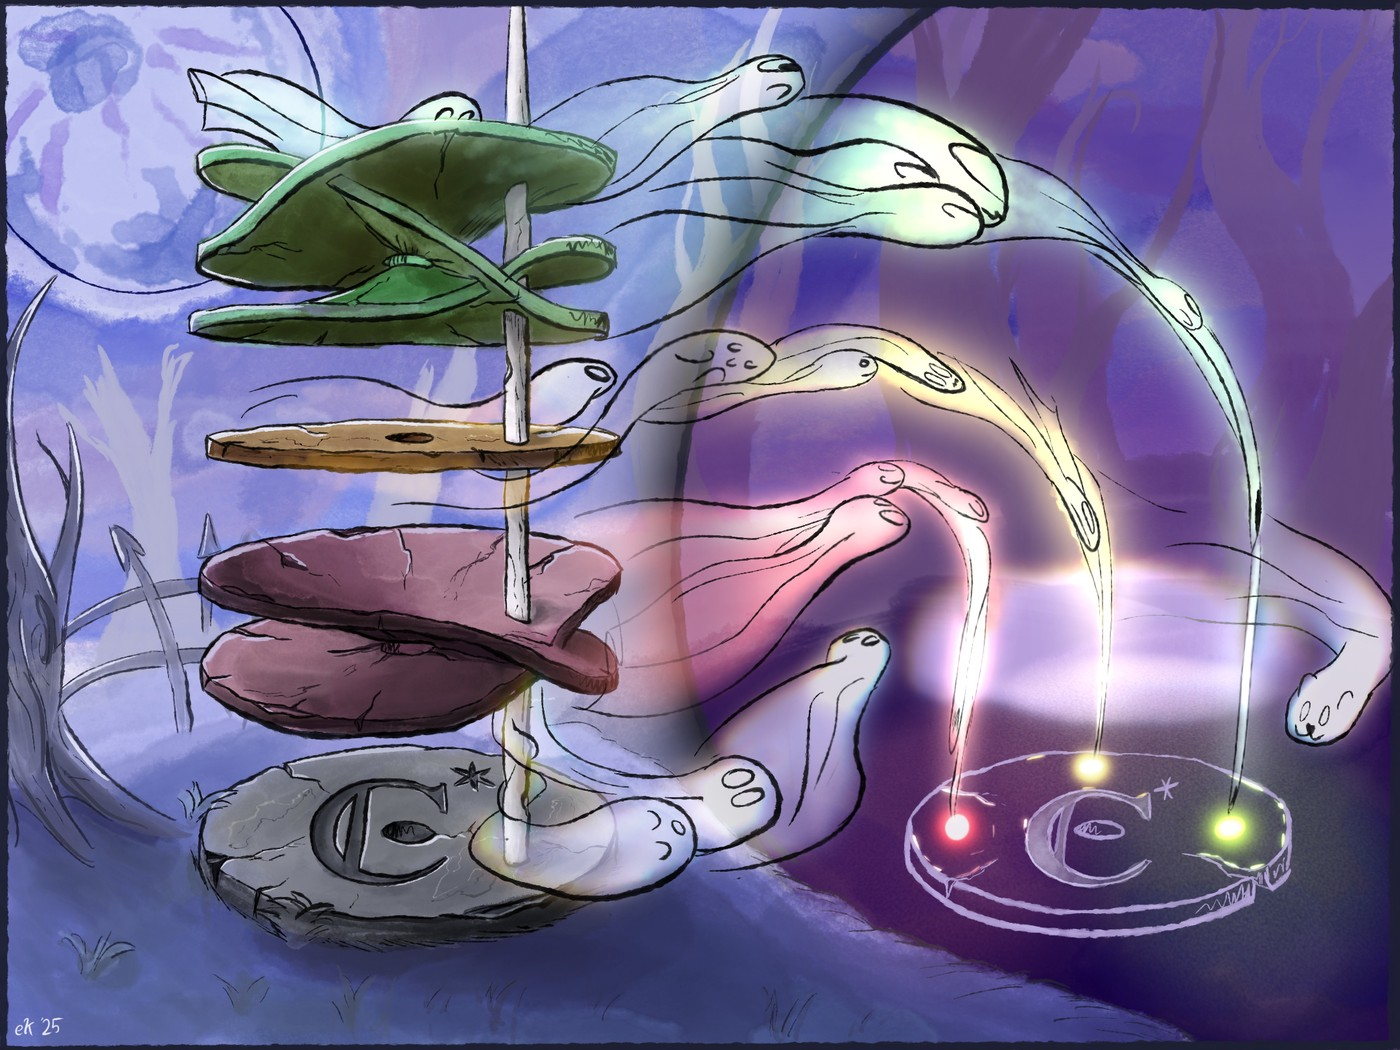
\includegraphics[width=0.74\linewidth]{figures/fig1.jpg}
\caption{层的梅林变换：谱把 $\C^{\times}_{z}$ 上的单色局部系统送到 $\C^{\times}_{t}$ 中的颜色。摩天楼对应于“白色”。（插图：Elliot Kienzle）}\label{fig:1}
\end{figure}

这些对象 $L_{t}\leftrightarrow L_{s}$ 特殊在哪里？$\C^{\times}_{z}$ 是一个群，而这些对象被称为特征层（character sheaf），因为它们的行为像这个群的特征——例如它们的解 $z^{s}$ 正好就是特征。我们可以这样表达这一想法：利用群结构，可以把局部系统沿 $w\in\C^{\times}$ 的旋转平移。$L_{t}=tz^{s}$ 是本征系统：由于 $(wz)^{s}=w^{s}z^{s}$，它们与自己的每个旋转 $w\in\C^{\times}$ 都相容地同构。对此的进一步阐发是：梅林变换把 $\Loc(\C^{\times}_{z})$ 上的卷积结构（表达 $\C^{\times}$ 的群结构）与 $\QCoh(\C^{\times}_{t})$ 上的乘法（即逐点张量积）结构等同起来。这样一来，它既是谱定理的一种形式，又是范畴化的傅里叶变换。

这契合范畴化傅里叶变换的总体主题——它们是阿贝尔群与其对偶之间各种层（导出）范畴的等价，互换卷积与张量积运算~[Lau96]。例子包括：在 $\C$、$\R$、$\F_{q}$ 上的对偶向量空间之间，分别等同 D-模、可构造层与 $\ell$-进层的 Fourier–Malgrange、Fourier–Sato 与 Fourier–Deligne 变换；以及在对偶阿贝尔簇之间等同凝聚层的 Fourier–Mukai 变换~[Muk81]。几何朗兰兹的挑战，就是为这一丰富的理论发展出非阿贝尔的对应物。

\subsection{非阿贝尔对偶的形状}\label{sec:1.4}

只要出现彼此交换的算子，傅里叶理论与谱定理的基本轮廓就适用。已知的非阿贝尔对应物则要受限得多、也精细得多。本节将勾画 Langlands 纲领与电磁 S-对偶所提供的非阿贝尔对偶的最粗略轮廓，以指出 GLC 在这两者之间所处的特殊位置。关于与物理的关系，另见 \S\ref{sec:6.2} 中略为宽广的提示。

\subsubsection{群}\label{sec:1.4.1}

我们首先固定

\begin{itemize}
\item $G$：一个约化代数群（reductive algebraic group）——例如 $\mathrm{GL}_{n}$、$\mathrm{SL}_{n}$、$\mathrm{SO}_{2n}$、$\mathrm{SO}_{2n+1}$……$E_{8}$。在 $\C$ 上（我们主要停留于此），这些正好是紧李群的复化。（我们只考虑连通群。）
\end{itemize}

每个这样的 $G$ 都伴随一个“对偶”的复\anote{更一般地，我们得到的是定义在 $G$ 的表示之定义域 $k$ 上的群——我们将假定（或假装假定）$k=\C$。}约化群，即朗兰兹对偶群（Langlands dual group）$\Gd$。关于 $\Gd$ 的总体想法是：$G$ 的各种花样的表示（即从 $G$ 出发的同态）应当对应于其对偶群中的共轭类——或更一般地，映入对偶群的同态。它可以借助李群的组合理论（根、Dynkin 图等等）具体定义：保留 $G$ 的外尔群，而把所有环面与根空间的组合结构对偶化。群 $\mathrm{GL}_{n}$ 与 $\mathrm{SO}_{2n}$ 是自对偶的；单连通群如 $\mathrm{SL}_{n}$ 与伴随群如 $\mathrm{PGL}_{n}$ 互换；奇正交群 $\mathrm{SO}_{2n+1}$ 则与辛群 $\mathrm{Sp}_{2n}$ 互换。我们将会看到，几何朗兰兹对偶给出了对偶群由何而来的根本性刻画，见 \S\ref{sec:3.3}。\zhnote{$\Gd$ 的组合定义只用到根数据（root datum）的对偶；nLab 词条 \emph{Langlands dual group} 给出了根数据对偶的完整定义与例子（$\mathrm{SL}_{n}\leftrightarrow\mathrm{PGL}_{n}$、$\mathrm{SO}_{2n+1}\leftrightarrow\mathrm{Sp}_{2n}$）：\href{https://ncatlab.org/nlab/show/Langlands+dual+group}{\texttt{https:/\allowbreak{}/\allowbreak{}ncatlab.\allowbreak{}org/\allowbreak{}nlab/\allowbreak{}show/\allowbreak{}Langlands+\allowbreak{}dual+\allowbreak{}group}}（最后修订 2014-09-07）。本译文统一作“朗兰兹对偶群”，首次出现后简称“对偶群”。}

\subsubsection{背景}\label{sec:1.4.2}

其次，我们需要选择背景。

\begin{itemize}
\item 电磁对偶涉及 4 维量子场论。对于它粗糙得多的拓扑形式（一种忽略一切动力学的“静态印记”），我们可以选任意维数不超过 4 的流形 $M$ 作为“时空”。
\item 对 Langlands 纲领，我们可以在几种“域”$F$ 中选一种：数域，如 $\Q$；局部域，如 $\R$、$\C$ 或 $\Q_{p}$；或一条（光滑射影）代数曲线 $C$ 上的有理函数域。对有限域 $\F_{q}$ 上的曲线 $C$，函数域 $F=\F_{q}(C)$ 的行为与数域非常相似。对代数闭域（如 $\F_{q}$ 或 $\C$）上的曲线 $C$，其函数域却出人意料地更像局部域。
\end{itemize}

GLC 发生在 $\C$ 上的光滑射影曲线 $C$ 上。我们同样可以把 $C$ 看作定义了一个紧黎曼面，特别是一个二维流形。因此它恰好同时嵌入这两个世界。

更一般地，两个世界之间有一种略显奇幻却极其有用的平行对应，即算术拓扑（arithmetic topology）的字典，或“纽结与素数”的类比~[Mor12]：数域与有限域上的曲线都被看作（3-流形的奇异亲戚），而局部域与代数闭域上的曲线则被看作 2-流形。

\subsubsection{对偶}\label{sec:1.4.3}

对每一组这样的输入——一个群 $G$ 与一个域 $F$ 或流形 $M$——都联系着一个对偶猜想。让我们试着在所有这些猜想中辨认出一般模式。一侧是“问题”：自守侧或 A-侧，它呈现一个与群 $G$ 及流形 $M$ 或域 $F$ 相联系的谱分解问题。这些问题以起初看来互不相干的奇异背景上的调和分析的形式出现——与数域相联系的局部对称空间 $[G]_{F}$、与代数曲线相联系的向量丛模空间 $\Bun_{G}(C)$，或 $M$ 上 Yang–Mills 方程解的模空间及其变体。值得注意的是，这些空间全都密切相关，而 GLC 正是沟通它们的桥梁，我们在 \S\ref{sec:2.2} 中讨论这一点。

另一侧是“答案”：谱侧或 B-侧。它用某个适当群（例如 $F$ 的伽罗瓦群，或 $M$ 的基本群）映入朗兰兹对偶群 $\Gd$ 的表示空间——即特征簇（character variety）$\Loc_{\Gd}$——的代数几何，来描述谱分解中可能出现的颜色。我们在 \S\ref{sec:2.3} 中讨论黎曼面／代数曲线这一 GLC 背景下的特征簇。

这些谱问题中最容易辨认的，也许要数局部 Langlands 对应（Local Langlands Correspondence, LLC）——对 $\R$ 或 $\Q_{p}$ 这样的局部域的对偶。这里自守侧由群 $G(F)$（一个实或 $p$-进李群）的所有光滑表示构成，与之相对的是关于 $\R$ 的（酉）表示的经典谱定理。LLC 试图把这些表示描述为 Langlands 参数空间 $\Loc_{\Gd}(F)$ 上的向量空间族（多重度空间），后者扮演谱定理中实直线 $\R_{t}$ 的角色。尽管 LLC 似乎不受其他背景中遇到的那些更为繁复的结构影响，过去十年间，通过把局部域视为曲线或二维流形的类比物、并引进来自 GLC 乃至最终来自物理的想法，这一领域已被彻底改变（最著名的是~[FS21]）。另见 \S\ref{sec:6.1.1}。

\subsubsection{问与答？}\label{sec:1.4.4}

把两侧标为“问题”与“答案”，传达了谱定理的心理学，也在很大程度上符合 GLC 中信息流动的方向：曲面的特征簇的几何，比模空间上层的调和分析初等得多。

然而在数域的背景下，典型的信息流向是相反的：伽罗瓦群及其表示是极其神秘而精细的对象，被用来表达数论中许多最深刻的问题，例如丢番图方程的解。把它们实现为模形式与自守形式的“颜色”，给出了算术不变量（如 $L$-函数）的一种截然不同的描述，并为来自表示论与分析的强有力工具打开了大门。

另一方面，在物理中，两侧之间的关系根本不同：量子场论中的电磁对偶是完全对称的关系，是单一理论的自同构，很像它所推广的傅里叶变换。这个自同构作用于理论的各种参数：耦合常数（交换弱耦合与强耦合）、规范群（交换 $G$ 与 $\Gd$），以及拓扑扭曲的选择——后者正是我们借以丢弃动力学、保留较粗糙拓扑信息的机制。等到我们考虑与 GLC 直接相关的拓扑场论之间的对偶时，A-侧看起来比 B-侧困难得多。然而这份来自物理的馈赠——两侧之间根本的平衡——依然处处可见，并渗透到非阿贝尔对偶的整个研究之中。\zhnote{“电磁对偶把 $G$ 换成 $\Gd$”在四维 $\mathcal{N}=4$ 超对称 Yang–Mills 中由 Montonen–Olive 对偶实现；Kapustin–Witten 进一步把它化为几何朗兰兹对偶，见 nLab 词条 \emph{S-duality} 与 \emph{Kapustin-Witten TQFT}：\href{https://ncatlab.org/nlab/show/S-duality}{\texttt{https:/\allowbreak{}/\allowbreak{}ncatlab.\allowbreak{}org/\allowbreak{}nlab/\allowbreak{}show/\allowbreak{}S-duality}}、\href{https://ncatlab.org/nlab/show/Kapustin-Witten+TQFT}{\texttt{https:/\allowbreak{}/\allowbreak{}ncatlab.\allowbreak{}org/\allowbreak{}nlab/\allowbreak{}show/\allowbreak{}Kapustin-Witten+\allowbreak{}TQFT}}（最后修订 2026-09-18）。}

\section{它说了什么？}\label{sec:2}

现在我们来更仔细地考察几何朗兰兹对偶的实际陈述。

\subsection{语言：勇敢新世界的调和分析与泛函分析}\label{sec:2.1}

我们论证过，谱定理关涉一个范畴，即 $\R$ 的酉表示——我们不仅有对象的集合，而且它们还彼此“交谈”。确实，表示论的基本研究对象就是范畴：它们作为群或代数的表示而出现，而目标是以有意义的方式描述它们，正如谱理论用本征空间把带自同态的向量空间搭建起来。

另一方面，\S\ref{sec:1.2} 中谱定理与傅里叶变换之间的类比——其中向量空间扮演数的角色，向量空间族扮演函数或测度的角色——提示我们把范畴本身看作希尔伯特空间的类比物。确实，范畴中的对象有一个“内积”，即它的 Hom 空间。当然，要成为一个希尔伯特空间，远不止一个带内积的集合——我们还有加法与数乘、拓扑与完备性。同样，我们要的不只是一个范畴，而是具有直和之类运算以及某种完备性概念的范畴。在这一类比中，同调代数取代了域 $k$ 上的线性代数：能够施行基本运算的那类性态良好的范畴，我们称之为导出范畴（derived category）（技术性的名称涉及三角 dg 范畴或 $k$-线性稳定 $\infty$-范畴之类的词）。这些基本例子由 $k$-代数的模范畴出发、“对同调代数的运算作完备化”而建成。同伦代数随后为泛函分析中的许多基本构造提供了对应物。

经典调和分析描述函数向量空间在对称群作用下的分解。近几十年来，一种丰富的范畴化调和分析已经浮现：其中函数向量空间被层的导出范畴（即各种取值于向量空间的“函数”）取代。例如，我们把 $z^{s}$ 这样的函数换成它们所满足的微分方程，如 $z\frac{d}{dz}-s$；把梅林变换这样的变换换成范畴上相应的函子。不断壮大的各种层论（又称六函子形式）为形形色色的函数空间提供了对应物。我们把一些松散的类比总结如下：\zhnote{“六函子形式”（six-functor formalism）指一套把层的推前、拉回、张量积、内 Hom、上同调与紧支撑上同调这六个操作公理化、并使之在导出范畴层面相容的形式体系；nLab 词条 \emph{six operations} 列出了这六个操作及其相容关系：\href{https://ncatlab.org/nlab/show/six+operations}{\texttt{https:/\allowbreak{}/\allowbreak{}ncatlab.\allowbreak{}org/\allowbreak{}nlab/\allowbreak{}show/\allowbreak{}six+\allowbreak{}operations}}（最后修订 2026-09-30）。原文所谓“brave new harmonic analysis”正是指：泛函分析里的积分、乘法、函数空间，在层论中分别对应推前／直积分、张量积、层的导出范畴。}

\begin{center}
\renewcommand{\arraystretch}{1.25}
\begin{tabular}{ll}
\toprule
泛函分析 & 范畴化的对应物\\
\midrule
向量空间 & 范畴\\
希尔伯特空间 & 导出范畴\\
算子 & （正合）函子\\
函数 & 层\\
积分 & 推前／直积分\\
乘法 & 张量积\\
函数空间 & 层的导出范畴\\
\bottomrule
\end{tabular}
\end{center}

GLC 的证明要求在一个全新的范畴化背景下，为泛函分析与调和分析的许多经典章节发展出对应物。这解释了本领域论文为何冗长而复杂，但也是这项事业对代数与解析几何、同伦论、数学物理与表示论等更广泛共同体的主要红利之一。由于其技术性，下文将尽量避免这种语言。

\subsection{背景：丛的模空间}\label{sec:2.2}

我们固定一个紧黎曼面（光滑复代数曲线）$C$，以及一个复约化群 $G$——读者不妨就把它取为可逆矩阵群 $\mathrm{GL}_{n}(\C)$，损失不大。我们将聚焦于非分歧的 GLC，即不在 $C$ 上打洞、也不在 $C$ 的点上添加额外数据。这是最基本的情形，也是已经被证明的情形，尽管大部分一般想法都有分歧版本。

主要研究对象是 $\Bun_{G}(C)$，即 $C$ 上代数（或全纯）$G$-丛的模空间（当 $C$ 不言自明时记作 $\Bun_{G}$）。这是代数几何中参数化 $C$ 上主 $G$-丛（即当 $G=\mathrm{GL}_{n}$ 时的秩 $n$ 向量丛）的对象。这意味着它不仅由点、而且由所有映入它的映射来定义——给出从簇 $S$ 到 $\Bun_{G}(C)$ 的映射，等同于给出 $S\times C$ 上的一个 $G$-丛。换言之，它是拓扑中分类空间在代数几何中的版本——具体说，它是从 $C$ 到 $G$ 的分类空间的代数映射空间。

这里先剧透一下结局：从几何（即点或经典力学）的角度看，空间 $\Bun_{G}$ 显得有些繁复巴洛克；但从它的线性化（即调和分析或量子力学）的角度看，它会显得漂亮得多。

\subsubsection{阿贝尔情形：雅可比簇}\label{sec:2.2.1}

要理解 $\Bun_{G}$，先考虑 $G=\mathrm{GL}_{1}$ 的情形，其研究可追溯到 Abel、Jacobi 与 Riemann。此时 $G$-丛与 $C$ 上的全纯线丛是同一份数据。经典地，线丛（或更确切地说，其全纯截面）由 $C$ 上的除子——$C$ 的点的整系数线性组合——给出，它确定一个在指定点至多取指定阶极点、至少取指定阶零点的亚纯函数空间。两个除子描述同一个线丛，当且仅当它们相差 $C$ 上某个实际有理函数给出的除子。

线丛的模空间 $\Bun_{\mathrm{GL}_{1}}(C)=\mathrm{Pic}(C)$ 就是 $C$ 的 Picard 群。关键事实已经出现：Picard 群在\emph{线丛张量积}这一运算下是一个阿贝尔群。更具体地，群结构由除子相加给出：$\mathrm{Pic}(C)$ 是除子群（以 $C$ 的点为基的自由阿贝尔群）对“整体”关系（来自亚纯函数的除子）的商。此外这个群有非常简单的描述：它是整数（给出除子的次数）与 $C$ 的雅可比簇的乘积
\[
\mathrm{Pic}(C)\;\cong\;\Z\times \mathrm{Jac}(C),
\]
而 $\mathrm{Jac}(C)$ 作为拓扑群是维数等于 $C$ 的亏格 $g$ 的环面，$\mathrm{Jac}(C)\cong(S^{1})^{2g}$。

\subsubsection{$\Bun_{G}$ 长什么样？}\label{sec:2.2.2}

现在来考虑 $G$-丛模空间的几何；对 $G=\mathrm{GL}_{n}$，它就是参数化 $C$ 上所有秩 $n$ 全纯向量丛的空间。图~\ref{fig:2} 给出了 $\Bun_{G}$ 的一幅图景。

\begin{figure}[tbp]
\centering
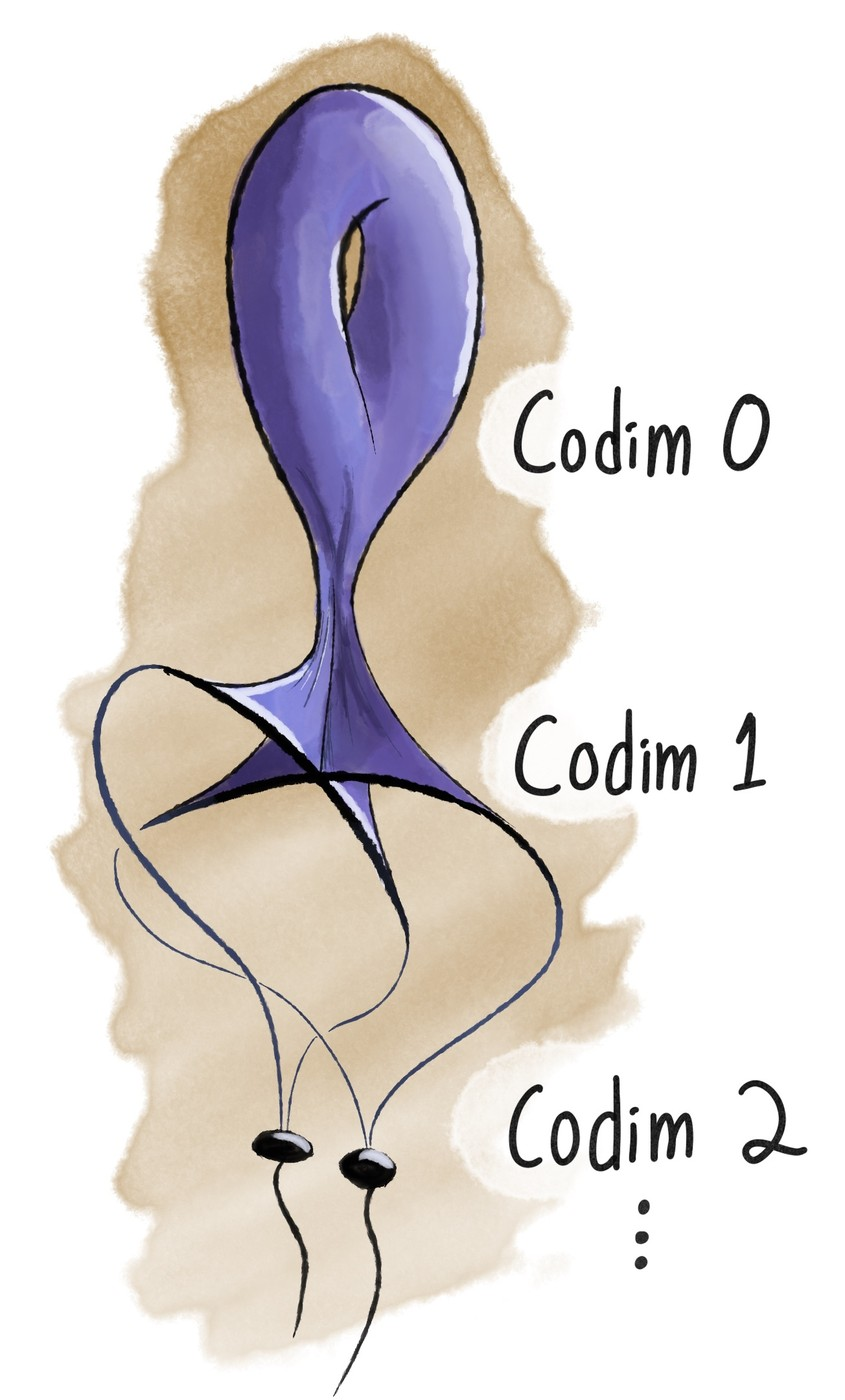
\includegraphics[width=0.34\linewidth]{figures/fig2.jpg}
\caption{$G$-丛模栈 $\Bun_{G}$ 的一幅图景：无限的“尾巴”由自同构越来越多的丛组成，核心则是半稳定丛。（插图：Elliot Kienzle）}\label{fig:2}
\end{figure}

这个空间比雅可比簇难对付得多：

\begin{itemize}
\item 第一，秩 $n$ 丛的集合上没有自然的乘法（对其他 $G$ 也没有），所以 $\Bun_{G}$ 不是群，更不是阿贝尔群。
\item 第二，$\Bun_{G}$ 不是簇，而是模栈（stack）——经典簇与分类空间的混合体。诗意地说，它是一个“点带有自同构群”的簇，因为丛可能有值得注意的自同构群。对雅可比簇而言，忽略这些自同构无伤大雅：所有线丛的自同构群都是同一个 $\C^{\times}$（于是只不过在 $\mathrm{Pic}(C)$ 连通分支的 $\Z$ 之外多一个同等的因子）。
\item 第三，与雅可比簇不同，$\Bun_{G}$ 的连通分支不是（拟）紧的。它包含一条无限的“尾巴”，由自同构越来越多的丛组成，这些丛通过在越来越大的次数范围内逐次扩张线丛而得到。这与模曲线（如椭圆曲线的模空间 $\mathbb{H}/\mathrm{PSL}_{2}\Z$）的尖点（以及由此产生的非紧性）密切类比。
\end{itemize}

在代数几何中，通常的做法是砍掉不稳定丛的尾巴，然后把半稳定丛的开核心坍缩到射影簇上——即几何不变量理论给出的半稳定 $G$-丛模概形。然而对 GLC 而言，保留带着全部“瑕疵”的完整 $\Bun_{G}$ 至关重要。第一，我们做的是表示论，丢弃内部对称群违背这门学科的全部精神；第二，半稳定丛构成的簇本身可能奇异（$\Bun_{G}$ 则不然），更关键的是，它的对称性更少：它不被 Hecke 对应（\S\ref{sec:3.1}）保持，而后者正是 Langlands 纲领最本质的特征。所幸尾巴具有良好的归纳结构，与核心的不可约本性形成对照：最“不紧”的部分纤维化到 $G$ 的极大环面的丛空间 $\Bun_{T}$ 上，而后者是若干 Picard 群的乘积。换言之，在尾巴的远端，丛由线丛的逐次扩张给出。一般地，尾巴类似地与其他 Levi 子群的丛相联系（在 $\mathrm{GL}_{n}$ 情形即分块对角矩阵——也就是低秩向量丛的逐次扩张）。

\subsubsection{除子？}\label{sec:2.2.3}

模空间 $\Bun_{G}$ 享有一个重要而微妙的对应物，可与用除子具体描述 $\mathrm{Pic}(C)$、用取指定零点与极点的函数描述线丛截面相类比。这就是：任何丛都可以在有限多个点之外被平凡化。于是，丛可以由“这种平凡化在每个这样的点附近如何失效”来描述。刻画这种失效的不再是一个整数，而是环路群
\[
\LG=\mathrm{Map}(D^{\times},G)
\]
（从去心圆盘映入 $G$ 的映射构成的环路群）对子群 $\LGp=\mathrm{Map}(D,G)$（能延拓到圆盘上的映射）的一个陪集。这个陪集空间 $\Gr=\LG/\LGp$ 就是仿射 Grassmannian（affine Grassmannian），即通常 Grassmannian 在环路群这一无穷维背景下的对应物。于是，我们可以这样指定一个丛：在曲线上指定有限多个点、并在每点标以仿射 Grassmannian 中的一个点（这是除子的类比），再对 $C$ 到 $G$ 的有理映射的作用取商（这是 $C$ 上有理函数的除子的类比）。因此 $\Bun_{G}$（像更熟悉的模曲线一样）有一个数论学家才熟悉的“阿代尔”描述，即双陪集空间
\[
\Bun_{G}=G(F)\backslash G(\mathbb{A}_{C})/G(\mathcal{O}_{\mathbb{A}_{C}})
\]
（这里 $F$ 是 $C$ 上的有理函数域）。这看起来笨重，却让人更深入地理解 $\Bun_{G}$ 的对称性。\zhnote{阿代尔描述与 Weil 单值化定理是同一个陈述：把 $G$-丛在有限多个点外平凡化，用 $G(F)$ 的作用把这些平凡化粘起来，剩下的自由度正是 $\prod'_{x}G(\C((z_{x})))$ 模 $\prod_x G(\C[[z_x]])$。nLab 词条 \emph{Weil uniformization theorem} 给出该双陪集分解的精确定义与它在几何类域论中的用法：\href{https://ncatlab.org/nlab/show/Weil+uniformization+theorem}{\texttt{https:/\allowbreak{}/\allowbreak{}ncatlab.\allowbreak{}org/\allowbreak{}nlab/\allowbreak{}show/\allowbreak{}Weil+\allowbreak{}uniformization+\allowbreak{}theorem}}（最后修订 2023-04-04）。}

对半单群 $G$（例如 $\mathrm{SL}_{n}$，即考虑行列式平凡的向量丛），这一描述有一个不那么“民主”却高效得多的变体。固定一点 $x\in C$，则 $\Bun_{G}$ 可以写成类似局部对称空间、类比于模曲线 $\Gamma\backslash\mathbb{H}=\Gamma\backslash \mathrm{SL}_{2}\R/\mathrm{SO}(2)$ 的形式：
\[
\Bun_{G}(C)=G(C\setminus x)\backslash \LG/\LGp,
\]
即单个仿射 Grassmannian 对从去心曲线映入 $G$ 的映射群取商。

\subsubsection{物理视角}\label{sec:2.2.4}

稍稍绕个弯：我要提一句，$\Bun_{G}$ 与黎曼面上 Yang–Mills 泛函的研究密切相关~[AB83]。最著名的结果是：半稳定 $G$-丛的模空间（由 Narasimhan–Seshadri 定理）作为 $C$ 上所有 $G$-规范场（联络）空间中 Yang–Mills 泛函的极小值空间出现。然而 Yang–Mills 泛函的临界点也包含不稳定丛，而该泛函的 Morse 理论控制着整个空间 $\Bun_{G}$ 的拓扑。于是 $\Bun_{G}$ 自然地出现在 $C$ 上量子 Yang–Mills 理论的研究中。这一关系正是 Langlands 纲领与规范理论之间联系的核心。

\subsection{谱侧}\label{sec:2.3}

GLC 的另一侧是 Langlands 参数空间，即 $C$ 上 $\Gd$-局部系统的空间 $\Loc_{\Gd}(C)$。这些空间扮演谱定理中频率或颜色空间 $\R_{t}$ 的角色，其点标记所有可能的“颜色”（本征值）。我们将在 \S\ref{sec:3.5} 中看到 Langlands 参数如何从 $\Bun_{G}$ 上调和分析的研究中作为“答案”有机地出现。

局部系统主要有两种风味，对应于傅里叶理论中对平移与微分的侧重：

\begin{itemize}
\item \textbf{Betti（群）版本}：$\Loc^{\Betti}_{\Gd}$ 本质上就是熟悉的特征簇（character variety），参数化 $C$ 的基本群映入 $\Gd$ 的表示（即当 $G=\Gd=\mathrm{GL}_{n}$ 时的 $n$ 维表示）。它是所有同态 $\pi_{1}(C)\to\Gd$ 构成的（轻度奇异的）仿射簇对 $\Gd$ 的（栈意义上的）商。具体地，对亏格 $g$ 的 $C$，可写
\[
\Loc^{\Betti}_{\Gd}(C)=\Bigl\{A_{1},B_{1},\dots,A_{g},B_{g}\in\Gd:\ \prod_{i=1}^{g}[A_{i},B_{i}]=1\Bigr\}\big/\Gd.
\]
于是对 $G=\Gd=\mathrm{GL}_{1}$ 这不过是 $(\C^{\times})^{2g}$\anote{更确切地说，还要模去自同构的栈性 $\C^{\times}$，并作某种“导出修正”以计入其定义方程的非横截性。}；而对亏格 $1$、$G=\Gd=\mathrm{GL}_{n}$，这是交换矩阵的共轭类空间。与标准特征簇概念的区别在于：正如 $\Bun_{G}$ 的情形，我们不仅记录点，还记录自同构——即考虑局部系统的栈，而不把它坍缩为底层的簇。
\item \textbf{de Rham（李代数）版本}：$\Loc^{\dR}_{\Gd}$ 参数化带平坦联络（flat connection）的 $\Gd$-丛，即向量场的李代数（而非基本群）的作用。于是对 $G=\Gd=\mathrm{GL}_{n}$，这是秩 $n$ 平坦向量丛的模空间。它（忘掉联络后）构成 $\Bun_{\Gd}$ 的某个拟紧开子集上的仿射丛（事实上它构成 $\Bun_{\Gd}$ 的余切丛的一个扭曲版本）。
\end{itemize}

平坦联络定义了平行移动的概念，即其单值性，从而定义了 $\pi_{1}$ 的一个表示。因此 $\Loc_{\Gd}$ 的 Betti 与 de Rham 两个版本在解析意义下相同，在代数意义下却不同——过渡到平行移动（解微分方程）是某种指数映射。例如对亏格 $1$ 的 $\mathrm{GL}_{1}$，前者是 $(\C^{\times})^{2}$，后者是椭圆曲线上的一个 $\C$-丛（一个著名的非仿射曲面，Serre 曾讨论过）。换言之，就点（或无穷小形变）而言两者无法区分，但在考虑局部系统的族时就必须小心。

下文将默认使用中性的记号 $\Loc_{\Gd}$ 表示两种风味的特征簇，凡可能时就隐去区别。

\subsection{几何类域论，或 $\mathrm{GL}_{1}$ 的 GLC}\label{sec:2.4}

让我们（重新）考虑雅可比簇 $\mathrm{Jac}(C)$，即 Picard 群 $\mathrm{Pic}(C)=\Bun_{\mathrm{GL}_{1}}(C)$ 的连通分支。它是阿贝尔群，因此可以在其上做傅里叶理论。具体说，我们可以把 \S\ref{sec:1.3} 的梅林变换描述本质上重复 $2g$ 次。代替可逆算子（即 $\Z$ 的表示）的谱定理，我们考虑 $2g$ 个彼此交换的可逆算子，即 $\Z^{2g}\cong\pi_{1}(\mathrm{Jac}(C))$ 的表示。可以把这些算子重新解释为雅可比环面 $\mathrm{Jac}(C)\cong(S^{1})^{2g}$ 上某个局部系统的单值性——即向量值函数沿 $2g$ 个方向可能的多值性。从谱的角度看，这 $2g$ 个交换算子描述 $2g$ 元洛朗多项式环 $\C[z_{1}^{\pm1},\dots,z_{2g}^{\pm1}]$ 上的一个模，或者更具启发性地，描述一族联合本征空间的代数族，即 $(\C^{\times})^{2g}$ 上的一个拟凝聚层。

另一方面，$(\C^{\times})^{2g}\cong\Loc_{\mathrm{GL}_{1}}(C)$\anote{同样忽略自同构的 $\C^{\times}$。} 是 $C$ 的秩一特征簇——即对 $C$ 中每个环路给一个纯量扭曲的数据。结果是一个等价，即 $\mathrm{GL}_{1}$ 的 Betti GLC：
\[
\Loc(\mathrm{Jac}(C))=\Rep(\Z^{2g})\;\overset{L}{\longleftrightarrow}\;\QCoh\bigl((\C^{\times})^{2g}=\Loc_{\mathrm{GL}_{1}}(C)\bigr).
\]
这个等价具有“傅里叶”性质：用雅可比簇的群结构作平移，被送到乘法（模的张量积）。虽然我们对等价的描述没有用到曲线的任何几何，$L$ 却满足一个自然的几何相容性。由 Abel–Jacobi 映射（即把点看作除子\anote{这个嵌入自然地落在次数为 $1$ 的分支 $\mathrm{Pic}^{1}(C)$ 中，但我们可以减去 $C$ 中一个选定的参考点，把它下移到 $\mathrm{Jac}(C)=\mathrm{Pic}^{0}(C)$，从而得到经典的 Abel–Jacobi 映射。}）给出的包含 $C\hookrightarrow \mathrm{Jac}(C)$ 在阿贝尔化意义下等同了基本群
\[
\pi_{1}(C)^{\mathrm{ab}}\cong\pi_{1}(\mathrm{Jac}(C)),
\]
而 $L$ 把 $\mathrm{Jac}(C)$ 上的秩一局部系统 $E$ 送到 $C$ 上相应的秩一局部系统处的摩天楼 $\OO_{AJ^{-1}(E)}$。这个性质正是（非分歧）几何类域论的特征性质：$L$ 让我们把 $\mathrm{Jac}(C)$ 的覆盖空间与 $C$ 的阿贝尔覆盖空间等同起来，并与 Abel–Jacobi 映射相容。\zhnote{几何类域论是 GLC 在 $G=\mathrm{GL}_{1}$ 时的情形，其经典形式即 Abel–Jacobi 映射给出的 $\mathrm{Pic}^{0}(C)\cong \Loc_{\mathrm{GL}_{1}}(C)$；nLab 词条 \emph{geometric class field theory} 把它表述为“曲线的基本群（阿贝尔化）与其 Picard 簇的基本群之等同”，并指出这正是高维几何 Langlands 的出发点：\href{https://ncatlab.org/nlab/show/geometric+class+field+theory}{\texttt{https:/\allowbreak{}/\allowbreak{}ncatlab.\allowbreak{}org/\allowbreak{}nlab/\allowbreak{}show/\allowbreak{}geometric+\allowbreak{}class+\allowbreak{}field+\allowbreak{}theory}}（最后修订 2025-05-11）。}

\subsubsection{D-模与 de Rham 共形场论}\label{sec:2.4.1}

与梅林变换一样，几何类域论也有 de Rham 版本。这里我们研究的不是局部系统，而是雅可比簇上的 D-模（D-module）。先提三种看待簇 $X$ 上 D-模 $\Dmod(X)$ 的方式：

\begin{itemize}
\item 在仿射簇 $X$ 上，D-模就是 $D(X)$——系数为多项式的微分算子环——上的模。当 $X$ 非仿射时（如我们关心的 $\mathrm{Jac}(X)$），多项式函数不够多，于是使用层论语言：D-模是对 $X$ 的开子集指派这样的模、并在重叠处给出等同的汇集。
\item 通过把 D-模用生成元与关系表示，可以重新解释为系数为多项式的线性偏微分方程组；同样，我们考虑开片上的这样的方程组，并在重叠处作等同。
\item D-模带有（多项式函数层）$\OO_{X}$ 的作用，也带有向量场李代数的作用，二者通过 Leibniz 法则相容。换言之，它是一个带有微分概念（即平坦联络）的拟凝聚层（向量空间的代数族）。
\end{itemize}

把 D-模看作以其解出现的广义函数的范畴化身是有益的，正如我们把 $\C^{\times}$ 上的方程 $z\frac{d}{dz}-s$ 看作其解 $z^{s}$ 的化身。我们将要寻找的单色 D-模（特征层或本征层）正是特殊函数的化身，并分享后者的许多丰富性质。

在雅可比簇上的所有 D-模中，有一类特殊的：带平坦联络的线丛。它们与 $\mathrm{Jac}$ 上的秩一局部系统一一对应，从而（由 Betti 等价）与 $C$ 上的秩一局部系统一一对应，最终与 $C$ 上带平坦联络的线丛一一对应。具体地，这个双射由在 Abel–Jacobi 映射下限制到曲线上给出。我们可以把这个双射解释为：把 $\mathrm{Jac}$ 上的一个 D-模对应到 de Rham 特征簇 $\Loc^{\dR}_{\mathrm{GL}_{1}}(C)$ 上相应点处的摩天楼。Laumon 与 Rothstein~[Lau96, Rot96] 证明了这一对应可以延拓为等价，即 $\mathrm{GL}_{1}$ 的 de Rham GLC：
\[
\Dmod(\mathrm{Jac}(C))\;\overset{L}{\longleftrightarrow}\;\QCoh\bigl(\Loc^{\dR}_{\mathrm{GL}_{1}}(C)\bigr),
\]
并满足与 Betti 版 $L$ 平行的类傅里叶性质。这个等价不如其 Betti 版本初等，部分原因是情形不那么仿射——两侧都不能简单地由单个环上的模给出。确实，该等价只在导出范畴层面成立：它是代数几何中典型的导出等价——Mukai 关于对偶阿贝尔簇上拟凝聚层导出范畴的著名傅里叶变换——的加强版本。尽管如此，对“一半”参数它可以变得非常具体而初等，这些参数平行于梅林变换情形中的基本微分方程 $z\frac{d}{dz}-s$。也就是说，我们可以（不用任何层论）通过指定所有全纯向量场的作用，在 $\mathrm{Jac}$ 上写出显式的一阶微分方程：
\[
t_{\xi_{i}}f=\mu_{i}f,\qquad i=1,\dots,g.
\]
它们对应于平凡线丛上所有平坦联络构成的 $g$ 维族 $d-\omega$，其中 $\omega$ 是 $C$ 上的全纯微分形式。

\subsection{终于，GLC}\label{sec:2.5}

现在我们可以描述 GLC 了——它是上一节几何类域论的非阿贝尔推广。GLC 通过线性化、即建立谱分解问题来研究模空间 $\Bun_{G}$。我们要作谱分解的对象——我们的“范畴化函数空间”——将是 $\Bun_{G}$ 上特定类型的向量空间层。$\Bun_{G}(C)$ 上的层可以看作 $G$ 的表示的 $\C$-类比：确实，如果把 $C$ 换成一个点，$G$-丛的栈就变成带 $G$-对称性的单点，其上的向量空间层正是 $G$ 的线性表示。

那么我们要考虑的是哪一类表示论，即自守层？主要有两种风味，de Rham 与 Betti，分别平行于谱定理用自伴算子（微分）与酉表示（平移）所作的表述：

\begin{itemize}
\item \textbf{de Rham（李代数）版本}：考虑 $\Bun_{G}$ 上的 D-模 $\Dmod(\Bun_{G})$。与任意簇上的 $\Dmod(X)$ 一样，它们定义为坐标片（即参数化 $C$ 上 $G$-丛族的仿射簇）上环 $D$ 的模（或线性偏微分方程组）的相容汇集。
\item \textbf{Betti（群）版本}：这里改而研究可构造层（constructible sheaf），即带沿道路平行移动数据的向量空间族。最基本的例子是局部系统，即 $\pi_{1}$ 的表示，它们来自求解平坦联络的平行移动问题（即描述单值性）。但在 $\Bun_{G}$ 的情形（不同于我们研究梅林变换或雅可比簇时），还需要允许更奇异的对象：只要求平行移动在“多数”方向上可逆。这样的对象出现在求解带特征方向的偏微分方程时，这些特征方向阻碍 Cauchy 问题的局部可解性。究竟允许哪些奇异性（沿幂零方向），其精确选择由表示论中的经验所指引，可追溯到 Harish-Chandra 与 Lusztig 分别关于李群表示与有限群表示之特征的工作，我们将在 \S\ref{sec:4.2} 中讨论。所得的范畴记作 $\Shv_{\Nilp}(\Bun_{G})$。
\end{itemize}

为避免记号累赘，除需要更明确交代背景之处，我们将把两个范畴都简记为 $\Shv(\Bun_{G})$。

主角既已登场，现在可以陈述 GLC 了：

\begin{theorem*}[GLC，[GR24a, ABC+24b, CCF+24, ABC+24a, GR24b]]\label{thm:glc}
存在范畴等价
\[
\Shv(\Bun_{G})\;\simeq\;\QCoh(\Loc_{\Gd}),
\]
de Rham 与 Betti 两种背景均成立，分别是~[BD, AG15] 与~[BZN18] 中的猜想。
\end{theorem*}

换言之，$\Bun_{G}$ 上的自守层——微分方程系统或其拓扑单值性数据——具有谱分解，可分解为 $C$ 的相应形式 $\Gd$-特征簇上的向量空间代数族。等价地，$\Bun_{G}$ 上有一族特殊的层，即单色对象或本征层，由 $\Loc_{\Gd}$ 的点参数化；而所有层都可以唯一地写成诸本征层的叠加。

几点简注：第一，如上陈述的定理并不完全正确——由于空间 $\Loc_{\Gd}$ 的奇异性，我们需要修改“代数族”的概念，把 $\QCoh$ 扩大为更奇异的变体 $\IndCoh_{\Nilp}$，见 \S\ref{sec:5.1}。\zhnote{$\IndCoh$（归纳凝聚层）与 $\QCoh$ 的差别在于：$\QCoh$ 只记录“函子性”中的拉回，而 $\IndCoh$ 同时记录推前与反常推前，因而能容纳奇异簇上的“错维”层。nLab 词条 \emph{ind-coherent sheaves} 给出其定义（$\IndCoh(X)$ 由有界凝聚层的归纳极限、再对拟凝聚层作某种完备化得到）以及与 $\QCoh$ 的比较：\href{https://ncatlab.org/nlab/show/ind-coherent+sheaves}{\texttt{https:/\allowbreak{}/\allowbreak{}ncatlab.\allowbreak{}org/\allowbreak{}nlab/\allowbreak{}show/\allowbreak{}ind-coherent+\allowbreak{}sheaves}}（最后修订 2015-10-05）。原文下标 $\Nilp$ 指“幂零奇异支撑”，见 \S\ref{sec:4.2}。}

第二，出于“泛函分析”的目的，我们处处都必须在导出范畴中工作——尽管这个等价惊人地接近于保持更熟悉的阿贝尔层范畴（特别是，本征层本身确实是层，而非层的复形~[FrR25]）。

第三，如上陈述的定理类似于把谱定理表述为两侧之间的抽象匹配，却完全没有刻画它（不像我们在阿贝尔情形中借助 Abel–Jacobi 相容性所作的那样），也没有指明它与实际本征值的联系——换言之，我们仍然遗漏了整个事业的要旨：这个等价必须对角化某个东西。这是我们下一个话题。

\section{它为何为真？跳动的心脏}\label{sec:3}

我们已经看到了 $\Bun_{G}$ 的大致形状。但它究竟特殊在哪里？为什么要在它上面做范畴化调和分析？关键的想法是：

\begin{quote}
\itshape
\textbf{几何朗兰兹的精髓：}线性化之后，$\Bun_{G}$ 的行为惊人地像一个阿贝尔群。
\end{quote}

关键在于：$\Bun_{G}$ 那些神奇的性质并不出现在考察其几何、即在点的层面时，而出现在它的调和分析或量子力学、即线性化之后，具体说，是在过渡到层的范畴之后。这个口号有两个深刻的体现，它们指引着整个领域：

\begin{itemize}
\item \textbf{Hecke 算子}：$\Bun_{G}$ 上的层带有一大批彼此交换的对称性，以卷积的方式作用。
\item \textbf{Hitchin 纤维化}：在微局部化、即从位置空间过渡到相空间之后，$\Bun_{G}$ 在一般情形下看起来像雅可比簇。
\end{itemize}

我们先讲第一个，它在根本层面上解释了对偶群与对偶本身从何而来。第二个我们留到 \S\ref{sec:4}，它要几何得多（代价是只在一般情形下有效），让我们能具体看到本征层长什么样。

\subsection{局部对称性：Hecke 算子}\label{sec:3.1}

要理解 $\Bun_{G}$ 的对称性，回忆 $\mathrm{Pic}(C)$ 上群结构的局部起源——除子相加——是有益的。给定线丛 $L$ 与点 $x\in C$，我们可以只在 $x$ 处修改 $L$：考虑被要求以某阶消失（或被允许以某阶取极点）的截面。换言之，我们可以给表示 $L$ 的除子 $\sum n_{i}x_{i}$ 加上 $x$ 的一个倍数。这给出 $\Z$ 的一个拷贝通过 $L\mapsto L(n\cdot x)$ 作用在 $\mathrm{Pic}(C)$ 上，而这些作用（对变化的 $x$）生成整个群结构。

这个 $\Z$ 的非阿贝尔对应物是什么？给定 $G$-丛 $P\in\Bun_{G}$ 与点 $x\in C$，我们首先应当参数化 $P$ 在 $x$ 处的所有修改，即在 $x$ 之外与 $P$ 等同的丛。这样的修改由双陪集 $\Gr=\LGp\backslash\LG/\LGp$ 刻画，即仿射 Grassmannian $\Gr$ 上的 $\LGp$-轨道。高斯消元的变体表明，这些轨道的集合与对偶环面 $\check T$（$G$ 的环面 $T$ 的对偶）的特征标在 Weyl 群作用下的轨道一一对应（对 $G=\mathrm{GL}_{1}$ 就还原为我们的 $\Z$）。换言之，由最高权理论，这些轨道与 Langlands 对偶群 $\Gd$ 的不可约复表示一一对应；$\Gd$ 正是按组合方式定义的、以 $\check T$ 为对偶环面且与 $G$ 有相同 Weyl 群的群。

但这些丛的修改不只是一个集合：修改可以复合。确实，群中的双陪集 $K\backslash G/K$ 本身并不带结合乘法，但线性化之后就带了。也就是说，群上的乘法通过卷积在群元素的加权组合（即群上的测度）上定义了一个结合代数结构（群代数）。这个结构在过渡到双陪集时仍然保留：群上的卷积在 $K$-双不变测度上给出一个结合乘法，即 $G$ 与 $K$ 的 Hecke 代数。

我们关心的是用层（而不是函数）来线性化群，即用 D-模或可构造层。把这一想法用到双陪集空间 $\Gr$ 上，就得到了球 Hecke 范畴
\[
\Sph_{G}=\Shv(\Gr)=\Shv(\Gr)^{\LGp},
\]
即 $\LG$ 上关于 $\LGp$ 的双陪集上的所有层构成的范畴；更具体（但不那么对称地），它是仿射 Grassmannian $\Gr$ 上关于 $\LGp$ 作用等变的层，或更具体地，$\Gr$ 上在每个 $\LGp$-轨道上为常值的层。换言之，Hecke 范畴中的对象是丛在一点处的各种可能修改的加权和，权重是向量空间。Hecke 范畴 $\Sph_{G}$ 从修改的复合（最终来自 $\LG$ 上的卷积）继承一个结合乘法——它构成一个幺半范畴。此外，$\Sph_{G}$ 通过卷积算子，即 Hecke 函子，作用在 $\Shv(\Bun_{G})$ 上：我们把层在 $P\in\Bun_{G}$ 处的值替换为它在该点处由修改得到的诸丛上的加权平均。这些是图 Laplacian 的近亲——把函数在图上的值替换为它在邻居上的平均。

在~[KW07] 的规范场论描述中——那是在量子场论的线性化框架中进行的——Hecke 函子被实现为 't Hooft 线算子：$P$ 在 $x$ 处的修改是通过在 $x$ 处的规范场中制造一个指定的奇异性来实现的，这对应于制造一个穿过 $x$ 的磁单极子。

\subsection{因子化：交换性之源}\label{sec:3.2}

GLC（可以说也是整个 Langlands 纲领）确凿无疑的跳动心脏是 Hecke 修改的奇妙交换性。一般的 Hecke 代数作为非阿贝尔群乘法的平均版本，本来没有理由交换。但磁单极算子的物理图像提示了另一种复合图景，即算子乘积展开（OPE）：我们可以在不同的、但彼此邻近的点上作相继的观测，然后取两点碰撞的极限。与量子力学本质上的非交换性不同，在更高维的量子场论中，算子有更多空间可以彼此绕行。在拓扑量子场论（测量沿形变保持不变）的框架中，这使算子的乘积交换。

同样的想法在代数拓扑中很熟悉：拓扑空间的高阶同伦群 $\pi_{2}$（或对 $n\ge2$ 的 $\pi_{n}$）之所以交换、而 $\pi_{1}$ 不交换，正是因为在一个带基点的空间中，我们可以让两个二维环路——把圆盘边界送到基点的映射——在更大圆盘的映射内部彼此绕行，这使得它们的复合在同伦意义下交换。这一观察是小圆盘（或 $E_{n}$）operad（乃至一般 operad）理论的起源，也是同伦论中交换性的主要来源。

这与我们何干？仿射 Grassmannian $\Gr$ 事实上同伦等价于分类空间 $BG$ 的二重环路空间：它被定义为曲面上的 $G$-丛空间，细看之下它描述的是在小圆盘外平凡化的丛，因而是到 $BG$ 的带基点映射。这意味着 $\Gr$ 本身带有同伦交换的乘法。

Beilinson 与 Drinfeld~[BD] 发现了这些来自物理与同伦论的机制的一个几何统一，称为因子化（factorization，同义地也称融合 fusion），它在 Hecke 范畴 $\Sph_{G}$ 背后起作用。也就是说，我们不必在同一点 $x\in C$ 处对丛作相继的 Hecke 修改（即用两个 Hecke 算子 $T_{1},T_{2}$ 作用），而可以在 $x$ 处作修改 $T_{1}$、在邻近的 $y$ 处作 $T_{2}$。球范畴的拓扑本性保证：当我们移动 $y$、或取 $y$ 与 $x$ 碰撞的极限时，复合在局部是常值的。让 $y$ 完全绕过 $x$ 一周，我们就得到了从复合 $T_{1}\circ T_{2}$ 到 $T_{2}\circ T_{1}$ 的一个形变。结论是：$\Sph$ 上的卷积乘积实际上是交换的——$\Sph$ 构成一个对称幺半范畴。

因子化——一种纯粹由流形上点的构型及其碰撞来几何地参数化、而非由传统的复合映射给出的代数结构——是一次真正革命性的发现，是几何朗兰兹研究中产生的最深刻、影响最大的思想。它的源头是 Segal、Beilinson 与 Drinfeld 为理解二维共形场论中算子乘积展开的几何意义所作的努力（这些在代数上被编纂为顶点代数与辫张量范畴的理论，那里“融合”一词更常用），以及它与代数拓扑中迭代环路空间（如 $\Gr$）与小圆盘 operad 的代数理论之间浮现出的密切平行。

在~[BD04] 中编纂之后，它为物理、拓扑、范畴论与数论中的现象提供了一个统一的视角。反过来说，在 Costello 与 Gwilliam~[CG17] 发展的一般数学框架中，因子化正是量子场论中可观测量的定义性特征。

Hecke 算子的交换性可以说是 Langlands 纲领最不可或缺的一面——没有可对角化的交换算子，就没有自守形式的谱分解。它背后是自守 $L$-函数的构造，并提供了把表示论与 Galois 理论联系起来的根本机制。然而这一交换性是通过一个技巧证明的，这个技巧既不能解释它为何成立，也不能说明如何把它变成一个稳固而可塑的原理。因子化恰好提供了这个原理，由它可以推出经典的交换性以及更多东西（通过去范畴化）。得益于 V.~Lafforgue、Fargues、Scholze、Zhu 以及许多其他人的开创性工作，它已成为算术背景中的基本工具。

\subsection{对偶群的诞生}\label{sec:3.3}

既然知道球 Hecke 范畴是交换的，我们就应当寻找 $\Sph$ 的傅里叶对偶描述——用张量积而非卷积的语言、即使其交换性显而易见的描述。更几何地说，我们应当寻找它的谱，即其作用的所有可能（联合）本征值构成的空间。这正是几何 Satake 对应的内容。已经有一个自然的猜测：我们注意到双陪集 $\Gr=\LGp\backslash\LG/\LGp$ 与 Langlands 对偶约化群 $\Gd$ 的不可约表示一一对应。于是人们可以期望用 $\Gd$-表示及其张量积来描述 $\Sph_{G}$ 的整个结构。下面的定理证实了这一猜测：

\begin{theorem*}[几何 Satake 对应；[Lus83, Gin, MV07]]\label{thm:satake}
存在对称幺半阿贝尔范畴的等价
\[
\Sph_{G}\;\simeq\;\Rep(\Gd),
\]
它把带卷积的球范畴与带张量积的 Langlands 对偶群 $\Gd$ 的表示范畴等同起来。
\end{theorem*}

\subsection{注}\label{sec:3.4}

该定理在~[MV07] 中被推广到系数取自任意域、甚至整数环的（反）周层（以及 $\Gd$ 的表示）。为简单起见，我们隐含地从导出范畴过渡到它们的核心（heart），即阿贝尔 $\C$-线性范畴，于是 $\Sph^{\heartsuit}$ 等价地由仿射 Grassmannian 上 $\LGp$-等变的 D-模或（反）周层构成。几何 Satake 还有对完整导出范畴的、重要而微妙得多的版本~[BF08]。

几何 Satake 对应或许最好反过来理解：它提供了 Langlands 对偶群 $\Gd$ 的真正定义。正如交换环定义了一个几何对象——它的谱，参数化该交换环所有可能的联合本征值——像 $\Sph$ 这样的交换张量范畴也有一个由 Tannaka 重构给出的谱。这参数化了所有可能的联合本征值，只不过这些本征值现在是向量空间而非算子。确实，对 $G=\Gd=\mathrm{GL}_{n}$，该定理可以转述为一个等价
\[
\{\Sph_{\mathrm{GL}_{n}}\ \text{的可能本征值}\}\;\longleftrightarrow\;\{n\ \text{维向量空间}\}.
\]
$n$ 维向量空间在同构意义下只有一个，但定理抓住了它的自同构群，即 $\Gd=\mathrm{GL}_{n}$。换言之，右端代表 $n$ 维向量空间的模栈 $\mathrm{pt}/\mathrm{GL}_{n}$。另一方面，对 $G=\mathrm{SO}_{2n+1}$（奇正交群），对偶群为 $\Gd=\mathrm{Sp}_{2n}$，定理说的是
\[
\{\Sph_{\mathrm{SO}_{2n+1}}\ \text{的可能本征值}\}\;\longleftrightarrow\;\{2n\ \text{维辛向量空间}\}.
\]
对一般的 $G$，答案由一点上的 $\Gd$-局部系统给出——那正是把 $\Gd$ 的任意表示变成向量空间、从而把 Hecke 算子变成本征值的机器。\zhnote{几何 Satake 对应的内容与 nLab 词条一致：$\Sph_{G}$ 是 $\LGp$-等变层构成的交换张量范畴，其 Tannaka 对偶（谱）正是 $\Rep(\Gd)$，于是对偶群 $\Gd$ 由 $\Sph_{G}$ 的自同构群重建出来；这正是 Tannaka 重构的几何版本，见 \emph{geometric Satake equivalence} 与 \emph{Tannaka duality} 两个词条：\href{https://ncatlab.org/nlab/show/geometric+Satake+equivalence}{\texttt{https:/\allowbreak{}/\allowbreak{}ncatlab.\allowbreak{}org/\allowbreak{}nlab/\allowbreak{}show/\allowbreak{}geometric+\allowbreak{}Satake+\allowbreak{}equivalence}}、\href{https://ncatlab.org/nlab/show/Tannaka+duality}{\texttt{https:/\allowbreak{}/\allowbreak{}ncatlab.\allowbreak{}org/\allowbreak{}nlab/\allowbreak{}show/\allowbreak{}Tannaka+\allowbreak{}duality}}（最后修订 2025-07-28）。}

为证明几何 Satake，我们先构造一个群，作为 $\Sph_{G}$ 上总上同调函子的自同构群（这个函子最终将对应于遗忘函子 $\Rep(\Gd)\to\mathrm{Vect}$）。然后有一个从 $\Sph$ 到该群表示的平凡张量函子，我们验证它是等价。这严重依赖于 $\Sph_{G}$ 的交换性，从而依赖于因子化。Grassmannian 及其 Schubert 分层的优美几何随后迫使这个群是约化的，并让我们算出其根系数据在组合意义下与 $G$ 的对偶，于是我们就有权把它叫作 Langlands 对偶群。

\subsection{整体对称性：谱作用}\label{sec:3.5}

借助几何 Satake 对应，我们现在有一大批交换算子作用在 $\Shv(\Bun_{G})$ 上——对每个点 $x\in C$，我们都得到一个交换张量范畴 $\Rep(\Gd)$ 的拷贝，而且它们彼此交换。换言之，我们找到了除子群 $\mathrm{Div}(C)=\bigoplus_{x\in C}\Z$ 作用在 Picard 群上的非阿贝尔对应物（这里的 $\Z$ 现在被理解为标记 $\mathrm{GL}_{1}(\C)\cong\C^{\times}$ 的不可约表示）。这提示我们也应找到除子之间作用于 Picard 群上的关系的对应物，即不同点处的修改如何相互作用。从谱的角度看，几何 Satake 描述的是单点处 Hecke 算子的谱，而现在我们需要理解由 $C$ 上所有点处的丛修改所生成的“整体 Hecke 代数”的谱。

关键仍然在因子化结构中：我们已经用一种把 $C$ 上邻近点的移动与碰撞包含在内的方式理解了 Hecke 算子的复合，所以只需理解从局部到整体的过渡。换言之，这一大批 Hecke 算子满足这样的关系：作用以局部常值的方式依赖于修改点 $x$，而在两个碰撞的点处作修改等同于在一点处复合修改。

这一非形式的想法被因子化代数的因子化同调这一概念精确捕捉。Beilinson–Drinfeld~[BD04] 的这一想法是顶点代数共形块理论的抽象化，如今为量子场论中整体可观测量如何由局部可观测量装配而成提供了一个有影响的数学模型~[CG17]，并在拓扑与高阶代数中作为经典同调理论的推广成为一个强大的多用途工具~[AF15, Lur]。\zhnote{因子化同调（factorization homology）是把因子化代数在流形上“积分”（即取张量积式的同调）所得的不变量；它在代数拓扑中的原型是 Ayala–Françis 对拓扑流形的构造。nLab 词条 \emph{factorization homology} 给出定义：对流形 $M$ 与因子化代数 $A$，$\int_{M}A$ 由把 $M$ 分解为小圆盘、在每块上取 $A(D)$、再沿嵌入取（高阶）余极限得到：\href{https://ncatlab.org/nlab/show/factorization+homology}{\texttt{https:/\allowbreak{}/\allowbreak{}ncatlab.\allowbreak{}org/\allowbreak{}nlab/\allowbreak{}show/\allowbreak{}factorization+\allowbreak{}homology}}（最后修订 2026-05-30）。原文强调的正是“局部数据 $\Rightarrow$ 整体可观测量”的装配机制。}

于是现在的挑战，与几何 Satake 对应时一样，是以对角化或傅里叶对偶的方式、用张量积而非卷积来描述球 Hecke 范畴的整体化（因子化同调）。换言之，我们要描述整体 Hecke 范畴的谱，即它所有可能的本征值构成的汇集。

自然的猜测又出现了。先考虑 $G=\mathrm{GL}_{n}$ 的情形。如前所述，$\Sph_{\mathrm{GL}_{n}}$ 在单点 $x\in C$ 处作用的可能本征值由 $n$ 维向量空间给出。上面的讨论于是提示：整体上应当有一族向量空间 $\{E_{x}\}_{x\in C}$，它们在 $x$ 上局部常值，即邻近点处的向量空间相互等同。这正是一个秩 $n$ 的 $C$ 上局部系统的数据，即特征簇 $\Loc_{\mathrm{GL}_{n}}(C)$ 的一个点——不同构的局部系统由它们沿 $C$ 中环路的单值性区分。更一般地，$C$ 上的 $\Gd$-局部系统 $E$ 正是把 $\Gd$ 的表示 $V$ 变成 $C$ 上局部常值向量空间族 $(V)_{E}$ 的机器。

这引向下述基本定理：

\begin{theorem*}[谱作用]\label{thm:spectralaction}
Hecke 作用 $\bigotimes_{x\in C}\Sph_{x}$ 在 $\Shv(\Bun_{G})$ 上的作用通过 $\QCoh(\Loc_{\Gd}(C))$ 的作用分解\anote{确切地说，映射 $\bigotimes_{x\in C}\Rep(\Gd)\to\QCoh(\Loc_{\Gd})$ 把 $x\in C$ 处的表示 $V\in\Rep(\Gd)$ 送到 $\Loc_{\Gd}$ 上的向量丛，其在局部系统 $E$ 处的纤维为 $(V)_{E}|_{x}$。}，de Rham~[Gai15] 与 Betti~[NY19] 两种背景均成立。
\end{theorem*}

与几何 Satake 对应一样，我们可以把这个结果转述为
\[
\{\Shv(\Bun_{G})\ \text{上 Hecke 算子的可能联合本征值}\}\;\longleftrightarrow\;\{C\ \text{上的}\ \Gd\text{-局部系统}\}.
\]

谱作用提供了几何朗兰兹对应中自守到谱的方向——它告诉我们，自守范畴可以在 Langlands 参数空间上作谱分解。遵循同样总体思路的谱作用变体现已在许多不同背景下得到证明，并构成本领域的若干最伟大成就，包括函数域上的 Langlands 对应~[Laf18, AGK+20] 与非阿基米德局部域上的局部 Langlands 对应~[FS21]。\zhnote{谱作用定理的“谱侧”是 $\QCoh(\Loc_{\Gd})$，其中 $\Loc_{\Gd}$ 是 $C$ 上 $\Gd$-局部系统的模栈；“作用”来自每个点 $x$ 处的几何 Satake 等价与 $\Rep(\Gd)$ 的对称幺半结构，经由因子化同调粘成整体。nLab 词条 \emph{geometric Langlands correspondence} 在“谱作用”一节给出的陈述与此一致：存在 $\QCoh(\Loc_{\Gd})$ 在 $\Shv(\Bun_{G})$ 上的作用，其单点情形即几何 Satake 等价：\href{https://ncatlab.org/nlab/show/geometric+Langlands+correspondence}{\texttt{https:/\allowbreak{}/\allowbreak{}ncatlab.\allowbreak{}org/\allowbreak{}nlab/\allowbreak{}show/\allowbreak{}geometric+\allowbreak{}Langlands+\allowbreak{}correspondence}}（最后修订 2026-04-11）。}

从规范理论的观点看，几何 Satake 对应把 $G$-丛理论中的自然局部可观测量（Hecke 磁单极算子）与对偶 $\Gd$-规范理论中由 $\Gd$-局部系统的单值性构造出的那些（Wilson 环路算子）等同起来。谱作用于是断言 $C$ 上的整体可观测量作用在 $\Bun_{G}$ 上的自守层上——换言之，它在可观测量的层面建立了电磁对偶的一个版本。

\section{如何使之具体？}\label{sec:4}

在这一节，我们的叙述在一条（余）切丛的岔路上分出去——简要谈谈 Hitchin 可积系统，它使几何朗兰兹的许多部分变得远为几何、远为具体。

\subsection{阿贝尔化，或希格斯机制}\label{sec:4.1}

微局部分析的一个重要教训是：函数的行为更接近相空间的几何（Wigner 分布、波前集以及偏微分方程的特征线都住在这里），而不只是位置空间的几何。因此，要理解如何在 $\Bun_{G}$ 上（乃至为何要）做调和分析，我们确实应当问：它的余切丛 $T^{*}\Bun_{G}$ 有什么特殊之处？图~\ref{fig:3} 给出了图示。

丛的模空间的余切丛本身也有模空间的解释，即 $G$-希格斯丛的模空间
\[
\Higgs_{G}(C)=\{P\in\Bun_{G},\ \eta\in\Gamma(C,\mathrm{ad}^{*}(P)\otimes\Omega^{1}_{C})\}:
\]
这些是丛连同希格斯场（Higgs field）的数据，后者是取值于自同态的一形式（共伴随丛扭以 $C$ 上的一形式所得的截面）。我们同样把 $\Higgs_{G}$ 当作模栈处理，并注意它像 $\Loc_{G}$ 一样轻度奇异。与 $\Bun_{G}$ 一样，它也有一个配对的子商，即半稳定希格斯丛的模空间；其研究由 Hitchin~[Hit87a] 开创，是 Corlette~[Cor88] 与 Simpson~[Sim92] 的非阿贝尔 Hodge 对应的主题。

作为余切丛，$\Higgs_{G}$ 有自然的辛结构（借助非阿贝尔 Hodge 理论，它在相应的半稳定模空间上细化为超 Kähler 结构）。Hitchin~[Hit87b] 发现它还带有一种华丽而稀有的几何结构，即完全可积的 Hamilton 系统；后者的诸实例还原了许多被研究得最多的可积系统。为简单起见，我们聚焦于 $G=\mathrm{GL}_{n}$ 的情形，尽管整个理论对其他群也有漂亮的推广，见~[DM96, DG02]。具体说，取取值于自同态的一形式的特征多项式，定义了一个映射
\begin{equation}\label{eq:hitchin}
\Hitch:\Higgs_{n}\longrightarrow\bigoplus_{i=1}^{n}\Gamma(C,\Omega^{\otimes i}_{C})
\end{equation}
从希格斯丛的模空间到一个向量空间。这个映射是 Lagrangian 纤维化，而一般纤维 $\Hitch^{-1}(\chi)$ 的连通分支是复环面（阿贝尔簇），如图所示。

事实上，一般纤维实际上是曲线上的 Picard 群（线丛的模空间）。希格斯场 $\eta$（作为取值于矩阵的一形式）的本征值切出一条曲线 $C_{\eta}\subset T^{*}C$，它是 $C$ 的 $n$ 重覆叠，称为谱曲线（spectral curve）。谱曲线的数据等价于特征多项式 $\chi(\eta)$ 的数据，所以我们可以把映射 $\Hitch$ 看作 $\eta\mapsto C_{\eta}$。纤维于是描述固定本征值下可能的诸本征空间；一般情形下它们是谱曲线上的一个线丛——因此纤维被等同于 Picard 群 $\Hitch^{-1}(\chi(\eta))=\mathrm{Pic}(C_{\eta})$。

另一方面，零纤维 $\Nilp=\Hitch^{-1}(0)$——整体幂零锥~[Lau88]——由 $\eta$ 为幂零矩阵的希格斯场构成（见图）。这是一个可约簇，包含零截面 $\Bun_{G}\subset\Nilp\subset T^{*}\Bun_{G}$ 作为希格斯场恒为零的那个不可约分支。

换言之，Hitchin 纤维化把 $\Bun_{G}$ 呈现为某条曲线的 Picard 群之退化中的一个分支——所以 $\Bun_{G}$ 在骨子里非常接近阿贝尔簇，就像 $\mathrm{GL}_{1}$ 的情形一样。这一 $\Bun_{G}$ 的阿贝尔形变背后的想法，是规范场论中著名的、用于质量生成与对称性自发破缺的希格斯机制之变体的几何实现：在那里，希格斯场 $\eta$（它带规范荷）取真空期望值 $\Hitch(\eta)$，从而把规范对称性破缺为 $\eta$ 的中心化子。

更引人注目的是，GLC 的谱侧与自守侧现在开始看起来非常相似：毕竟，向量丛上的联络是取值于自同态的一形式的扭曲版本。具体说，模空间 $\Loc^{\dR}_{\Gd}$ 在一个单参数族中退化到 $\Gd$-希格斯丛的空间 $\Higgs_{\Gd}=T^{*}\Bun_{\Gd}$。Hausel–Thaddeus~[HT03] 与 Donagi–Pantev~[DP12] 的发现是：Langlands 对偶群的 Hitchin 系统一般地构成同一向量空间上互为对偶的阿贝尔簇族——用物理的语言说，它们互为 SYZ 镜像（见近期的综述~[Hau23]）。确实，[DP12] 证明：在 Hitchin 基上的一般点处，有一个等价，即 Dolbeault GLC
\begin{equation}\label{eq:dolbeault}
\QCoh(\Higgs_{G})\ \longleftrightarrow\ \QCoh(\Higgs_{\Gd}),
\end{equation}
它在纤维上由对偶阿贝尔簇上凝聚层的傅里叶–Mukai 变换~[Muk81] 的变体给出。（这个等价的适用范围随后在~[Ari13, MRV19a, MRV19b] 中被扩展，尽管关于整个 Hitchin 系统的完整图景仍未可得。）这提示 GLC 应当物理地表现为（同调）镜像对称的一种形式，而这确实在~[KW07] 中得到确认。

\begin{figure}[htbp]
\centering
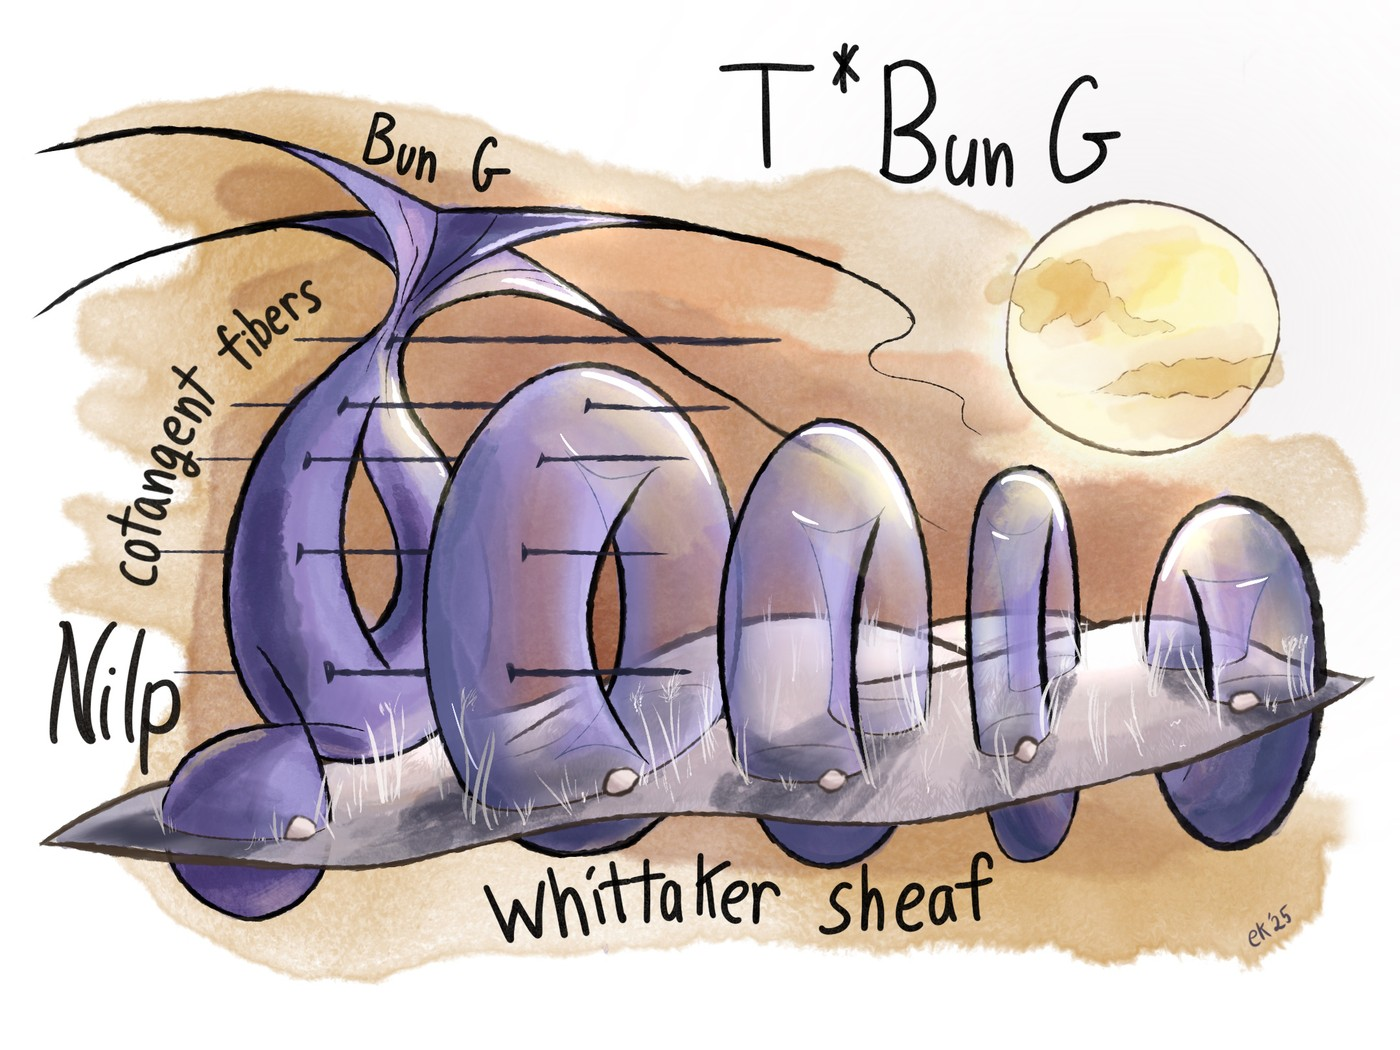
\includegraphics[width=0.78\linewidth]{figures/fig3.jpg}
\caption{希格斯丛模空间的 Hitchin 纤维化，图示零纤维（幂零锥，含 $\Bun_{G}$）与 Hitchin 截面（Whittaker 层的微支撑）。}
\label{fig:3}
\end{figure}

\subsection{层的阿贝尔化}\label{sec:4.2}

Hitchin 系统的几何与自守层理论有何关系？代数分析给出的一个重要洞见是：层就像广义函数一样，本质上具有微局部的性质，其支撑落在相空间中。因此，如 Donagi 首先建议的那样，我们可以用“阿贝尔化”的途径来处理 GLC：借助 Hitchin 纤维化的几何，把 $\Bun_{G}$ 上的层论“一般地”化归为 $\mathrm{GL}_{1}$ 的情形。\zhnote{“微局部”与“奇异支撑”是这块内容的技术核心：一个层（或 D-模）的奇异支撑是相空间 $T^{*}X$ 中的子簇，记录函数（层）在哪些点与哪些方向上不光滑、不“光滑可延拓”，它是物理中波前集的代数对应物；对 D-模而言它与特征簇在 Riemann--Hilbert 对应下相合。nLab 的 \emph{singular support} 页面实际重定向到“分布的支集”，义项不同，故此处不作链接；相关概念可自上而下的入口是 \emph{characteristic variety} 词条，\href{https://ncatlab.org/nlab/show/characteristic+variety}{\texttt{https:/\allowbreak{}/\allowbreak{}ncatlab.\allowbreak{}org/\allowbreak{}nlab/\allowbreak{}show/\allowbreak{}characteristic+\allowbreak{}variety}}（最后修订 2017-08-29）。}

图景如下：在傅里叶理论中，单色波（指数函数 $e^{i\lambda x}$）在动量空间中是局部化的，因此在微局部看来像 $\mathbb{R}^{2}_{x,t}$ 中的直线 $\{t=\lambda\}$。同样，我们可以期望所求的本征层——$\Bun_{G}$ 上的“单色”层——沿 Hitchin 纤维微局部地局部化，从而可以通过阿贝尔对偶来把握。把 Hitchin 纤维替换为它们在余切丛中按伸缩取极限后的版本，我们得到这一陈述的一个更粗糙的渐近版本：本征层应当以整体幂零锥 $\Nilp=\Hitch^{-1}(0)$ 为其特征簇~[Lau87]。（这在很大程度上解释了为什么在 Betti GLC 的表述中，带有幂零奇异支撑的层是应当考虑的正确推广（\S\ref{sec:2.5}））。

在他们引入我们所知的 GLC 的巨著~[BD] 中，Beilinson 与 Drinfeld 证明：Hitchin 的 Hamilton 量（$\Bun_{G}$ 上由 Hitchin 基上线性函数拉回的函数）可以形变为 $\Bun_{G}$ 上整体定义的交换微分算子\anote{差一个由自旋结构给出的扭。}。这些微分算子的本征系统给出 $\Bun_{G}$ 上一族整体定义的微分方程组（D-模），它们在微局部对应于 Hitchin 纤维上的常值层（不带任何缠绕）。它们是 \S\ref{sec:1.3} 中 $C^{\times}$ 上微分方程 $z\frac{d}{dz}f=sf$，以及 \S\ref{sec:2.4.1} 中雅可比簇上整体定义的 D-模族 $\{t_{\xi_{i}}f=\mu_{i}f\}_{i=1}^{g}$ 的非阿贝尔推广。

此后出现了若干把 GLC 的大部分阿贝尔化的途径：

\begin{itemize}
\item \textbf{渐近展开}：第一，微分算子有半经典极限，此时它们退化为其象征（symbol），即相空间上的函数。这提示了下述由 Arinkin~[Ari05] 发展的想法：
\begin{equation}\label{eq:asymp}
\Dmod(\Bun_{G})\ \rightsquigarrow\ \QCoh(\Higgs_{G})\ \longleftrightarrow\ \QCoh(\Higgs_{\Gd})\ \rightsquigarrow\ \QCoh(\Loc_{\Gd}).
\end{equation}
过渡到象征把 $\Bun_{G}$ 上的 D-模退化为 $\Higgs_{G}$ 上的拟凝聚层。然后我们用 Dolbeault GLC \eqref{eq:dolbeault} 从 $\Higgs_{G}$ 过渡到 $\Higgs_{\Gd}$，最后从 $\Higgs_{\Gd}$ 形变到 $\Loc_{\Gd}$。这给出了 GLC 的一个“一般的、形式渐近的”片段。
\item \textbf{谱侧的阿贝尔化}：上述联络的形式 WKB／半经典描述有一个引人注目的整体形式，由 cluster 簇的理论与超对称量子场论~[FG06, GMN13] 提供。这用环面坐标卡给出了局部系统空间 $\Loc_{\Gd}$ 的阿贝尔化描述，而这些卡来自覆叠空间上的秩一局部系统。
\item \textbf{模 $p$ 约化}：把微分算子模素数 $p$ 约化也有经典极限的效果（因为 $p$ 次导数模 $p$ 消失，于是环 $D$ 模 $p$ 变得非常接近其象征）。结果是可以把 $C$ 上的平坦联络与 $\Bun_{G}$ 上的 D-模直接与它们的 Dolbeault 对应物联系起来。这给出了 de Rham GLC 的模 $p$ 形式中一般部分的证明，其方法是约化到 Dolbeault 情形，如~[BB07, CZ17] 所完成的那样。
\item \textbf{Fukaya 范畴与微局部层}：Kapustin–Witten 提议把自守层放在辛几何与镜像对称的语境中看作 $T^{*}\Bun_{G}$ 上的 A-膜，即 Fukaya 范畴的对象。这些对象恰好由配备局部系统的 Lagrangian 表示。其中包括带局部系统的 Hitchin 纤维，它们给出了 Hecke 本征层的具体几何实现。这对后来借助微局部层论~[NZ09, Nad09, Kon09, GPS24] 理解 Fukaya 范畴产生了巨大影响。我们将看到这些想法出现在 GLC 的证明中（\S\ref{sec:5.4}）。
\item \textbf{非阿贝尔 Hodge 理论}：最后，非阿贝尔 Hodge 理论（由 Simpson、Mochizuki 等人发展）导向一种关于 GLC 的深刻视角，正由 Donagi–Pantev–Simpson 发展（综述见~[DP09]，另见~[DP22, DPS24]）。簇 $X$ 上的非阿贝尔 Hodge 对应用调和映射理论把合适的平坦联络、或更一般的 D-模，与希格斯层、即 $T^{*}X$ 上的凝聚层等同起来。$C$ 上的非阿贝尔 Hodge 理论造就了希格斯丛与局部系统模空间深刻的超 Kähler 几何，而 $\Bun_{G}$ 上的非阿贝尔 Hodge 理论则直接从 Hitchin 纤维上的线丛（视为希格斯层）构造出特殊的 Hodge（或 twistor）D-模。这为完成 \eqref{eq:asymp} 中从局部系统到 D-模的翻译提供了另一条途径。另见 \S\ref{sec:6.2}。
\end{itemize}

\section{它是如何被证明的？}\label{sec:5}

在这一节，我描述进入 GLC 证明的一些主要想法。

\S\ref{sec:3.5} 的谱作用告诉我们，可以在 Hecke 算子的作用下对自守范畴 $\Shv(\Bun_{G})$ 作谱分解，可能的颜色（Langlands 参数）由 $\Gd$-局部系统、即特征簇 $\Loc_{\Gd}$ 的点提供。既然如此，我们就可以表述“最佳情形”：

\begin{itemize}
\item Hecke 算子有简单的联合谱（量子完全可积性），且
\item 每一种可能的颜色都出现，即谱恰好是整个 Langlands 参数空间 $\Loc_{\Gd}$。
\end{itemize}

换言之，我们可以期望所有联合本征空间的重数都为一，从而对每种颜色 $E\in\Loc_{\Gd}$ 都有唯一（在归一化意义下）的本征层 $\mathrm{Aut}_{E}\in\Shv(\Bun_{G})$。本征层条件是说，每个 Hecke 算子 $F\in\QCoh(\Loc_{\Gd})$ 通过乘以向量空间 $F_{E}$（即 $F$ 在 $E$ 处的纤维）作用在 $\mathrm{Aut}_{E}$ 上：
\[
F*\mathrm{Aut}_{E}\;\simeq\;F|_{E}\otimes\mathrm{Aut}_{E}.
\]
合起来，我们可以把这一期望表述为：谱作用 $\QCoh(\Loc_{\Gd})\curvearrowright\Shv(\Bun_{G})$ 是秩一的自由作用，于是归一化之后我们期望得到如下形式的谱定理：
\[
\Shv(\Bun_{G})\;\simeq\;\QCoh(\Loc_{\Gd}).
\]
回忆一下：线性算子有简单谱，当且仅当它有循环向量。因此我们可以把这一期望转述为：Hecke 作用有循环向量（确切说，循环对象），并且这个循环向量有满谱支撑，即它是所有颜色的叠加。换言之，我们要找一个对象 $\mathrm{White}_{G}\in\Shv(\Bun_{G})$，它具有白光的性质；一旦找到它，GLC 就应当由下面两条唯一刻画：

\begin{itemize}
\item \textbf{谱作用}：等价 $\Shv(\Bun_{G})\simeq\QCoh(\Loc_{\Gd})$ 保持 $\QCoh(\Loc_{\Gd})$ 的作用；
\item \textbf{归一化}：该等价互换 $\mathrm{White}_{G}$ 与 $\OO_{\Loc_{\Gd}}$。
\end{itemize}

\subsection{先做一点泛函分析}\label{sec:5.1}

这个“最佳情形”原来需要一些修正——也就是说，我们必须把泛函分析做对。

既然 GLC 关涉的是一种以层的范畴取代传统函数空间的调和分析，我们理应遇到熟悉的分析问题的回声——反过来说，GLC 为这种新的范畴化分析提供了试验场。与局部对称空间的调和分析一样，首要问题来自（拟）紧性的缺失——即，我们应当在尖点处施加什么样的增长条件？这些选择导向什么类的“拓扑向量空间”，它们带有何种对偶与算子理论？在范畴化背景下，这些问题又究竟意味着什么？

这些问题在 Gaitsgory 与 Drinfeld、Arinkin 合作的系列论文（包括~[DG13, DG15, Gai16, Gai17b, AG15]）中得到发展，其基础是 Lurie 发展的范畴机器~[Lur09, Lur]。一方面，他们确立了 de Rham GLC 中的基本函数空间，即范畴 $\Dmod(\Bun_{G})$，“奇迹般地”表现得像范畴化的希尔伯特空间——特别是它是自对偶的。另一方面，对谱侧的朴素猜测需要精化。在傅里叶理论中，紧支撑的缺失对偶于光滑性的缺失。因此，如果我们选择不对 $\Bun_{G}$ 上的层施加任何增长条件，就应当预期在 $\Loc_{\Gd}$ 上的层论中出现奇异性——即某种取值于向量空间的“分布”，而非“函数”。事实证明，层层面上的这一区别与底空间 $\Loc_{\Gd}$ 的奇异性密切相关。

这引出了代数几何中内容丰富的新篇章，即归纳凝聚层理论 $\IndCoh$~[GR17]。范畴 $\IndCoh$ 把 $\QCoh$ 扩大以容纳代数广义函数。与分布一样，这些新对象可以描述为在“测试”对象上的泛函——在这里是凝聚层上的函子。$\IndCoh$ 与 $\QCoh$ 的差别归结为：奇异簇上的凝聚层——例如奇异点处的摩天楼——不允许由向量丛给出的有限分解，或更几何地说，不能延拓到簇的任意无穷小形变。这引出了归纳凝聚层的奇异支撑这一概念——分布的波前集的精确对应物——它度量给定的广义层在哪些点与哪些形变方向上受到阻碍。

通过分析奇异支撑在层的自然操作下的行为，[AG15] 得以精确调校出：究竟何种类型的归纳凝聚层奇异性与自守侧给定的层论相匹配——我们应当允许幂零奇异支撑\anote{值得注意的是，这一概念与加在自守侧 Betti 层上的、名字相近的幂零支撑条件并无密切关系。}，这大致意味着不允许来自环面方向的任何奇异性（如同先前已理解的 $\mathrm{GL}_{1}$ 情形）。这最终导向非分歧几何 Langlands 猜想的精确陈述：它是一个等价
\[
\Shv(\Bun_{G})\;\simeq\;\IndCoh_{\Nilp}(\Loc_{\Gd})
\]
（de Rham 与 Betti 两种风味均如此），它把左侧 $\QCoh(\Loc_{\Gd})$ 的谱作用与谱侧自然的张量作用（在广义函数上乘以函数）等同起来。

\subsubsection{étale 背景}\label{sec:5.1.1}

里程碑式的论文~[AGK+20] 引入了 GLC 的一种新风味，即 étale（或受限）版本。它最重要的优点或许是：它在任意代数闭域上都有意义，从而第一次在正特征函数域的背景下表述了范畴化的 GLC，并建立了相应的谱作用。在 $\C$ 上，étale 版本构成 Betti 与 de Rham 猜想之间的中间“共同核心”。例如在谱侧，$\Loc^{\Betti}_{\Gd}$ 与 $\Loc^{\dR}_{\Gd}$ 有相同的点，且这些点有相同的形变理论，所以两者所有点的所有形式邻域之并是相同的。特征簇的 étale 版本恰好就是（对阿贝尔群而言）这个并，一般情形下则稍大一些（本质上是因为对幂零矩阵取指数是一个代数操作）。特别是，由摩天楼经有限过程搭出的凝聚层在三个版本上都是相同的。对偶地，étale 自守范畴被设计成由单色对象离散地、而非连续地搭成。

论文~[AGK+20] 证明了 GLC 的 Betti 与 de Rham 版本彼此等价：它表明两者都化归到共同的 étale 版本。这让我们可以交替利用两种背景的优势——例如，Betti 特征栈 $\Loc^{\Betti}_{\Gd}$ 非常简单，是仿射簇对 $\Gd$ 的商，明显地只依赖于 $C$ 的拓扑；而 de Rham 版本 $\Loc^{\dR}_{\Gd}$ 远非仿射，于是凝聚层之间的 Hom 空间是有限维的。

\subsection{间奏：相对 Langlands，或 $L$-函数都去哪儿了？}\label{sec:5.2}

Langlands 哲学所预言的并不只是自守侧与谱侧之间使 Hecke 算子对角化的一个关系：它还配备了庞大的预测体系，说明什么样的测量应当与什么样的测量相匹配。对这些测量的研究称为相对 Langlands 纲领，并在~[SV17] 中被系统化。最著名的一项——把自守表示与 Galois 表示相联系的 $L$-函数的匹配——可以说是算术 Langlands 纲领的主要特征。$L$-函数本身在 GLC 的大部分文献中显著地缺席，但类似的匹配测量在归一化、刻画与证明 GLC 中起着主要作用。

自守形式的“测量”是什么意思？它们是自守形式向量空间上的线性泛函——不过我们也可以（并且将会）对偶地把它看作与某个特定向量的内积，或在几何语境中看作从某个特定层出发的 Hom 空间。我们可以为之作出预测的特殊测量——周期（period）\anote{容易混淆的是，不要与代数几何中的“周期”混为一谈。}——是高度结构化的：它们在 Langlands 纲领的所有不同背景（局部、整体、算术、几何）中都有对应物，并满足很强的相容性。

在物理中，这种结构化的测量或状态集合是任何量子场论的本质部分，它们对应于边界理论（或余维一的缺陷）。更具启发性的是，我们可以通过规范场论与带电物质的相互作用来研究它。在电磁 S-对偶的语境中，Gaiotto–Witten~[GW09b, GW09a] 开创了这类研究，并在~[BZSV24] 中被提议为相对 Langlands 纲领的一般框架（另见~[Gan]）。\zhnote{“周期”在 Langlands 语境中不应与代数几何的周期（周期积分）混淆：它指自守形式上的某种不变线性泛函，即把自守表示“求值／积分”得到一个数或向量空间。相对 Langlands 纲领（Relative Langlands）就是系统研究这些周期、并把它们与谱侧相应的“测量”相匹配的理论；nLab 词条 \emph{relative Langlands program} 给出的正是这一观点：\href{https://ncatlab.org/nlab/show/relative+Langlands+program}{\texttt{https:/\allowbreak{}/\allowbreak{}ncatlab.\allowbreak{}org/\allowbreak{}nlab/\allowbreak{}show/\allowbreak{}relative+\allowbreak{}Langlands+\allowbreak{}program}}（最后修订 2025-04-29）。}

一个基本例子是平凡周期——常数波或零频波，它对应于最简单的测量：取自守形式的平均，或取自守层的整体上同调。这个周期在 GLC 的语境中已经非常有趣：它在~[GL19b] 中得到研究，并被用来证明函数域的 Weil 玉河数猜想。

下面三节中，我们来看三种重要的测量（周期），它们的相互作用构成了 GLC 证明的骨架（转述自~[CCF+24]）。这里列出相匹配的自守测量与谱测量的名称及其主要作用：

\begin{itemize}
\item \textbf{Eisenstein $\leftrightarrow$ Eisenstein}：在 GLC 上提供归纳结构，把猜想化归到尖点情形。
\item \textbf{Whittaker $\leftrightarrow$ 整体截面（Neumann）}：用于归一化——提供对尖点自守层的忠实测量。
\item \textbf{Kac–Moody $\leftrightarrow$ opers}：用于构造尖点自守层。
\end{itemize}

周期的可能最关键的特征是：它们满足很强的局部–整体相容性——它们由 $\Theta$-级数给出。$\Theta$-级数（或 Poincaré 级数）是经典 Riemann $\theta$-函数的推广，后者例如出现在 Riemann 关于 $\zeta(s)$ 的积分公式中。它们是模形式与自守形式，写成局部数据在一个整体对称群上的平均。这事实上是写出自守形式最常见的方式之一。

$L$-函数的一个特征性质是它们作为 Euler 乘积的“局部–整体”描述。在几何背景中，周期有一个松散类比的关键性质——又是因子化。也就是说，我们可以把 $\Theta$-级数附着到曲线 $C$ 上有限多个点处的局部数据上，而构造与点的碰撞相容。这一因子化性质是把局部输入装配成可理解的整体输出的胶水。它在技术上也极具挑战——GLC 证明（及其许多前身）之所以冗长，一个主要原因是需要整体地理解所有构造的局部、整体与可因子化版本。

\subsection{归纳步：Eisenstein 级数}\label{sec:5.3}

Eisenstein 级数同时是自守形式理论中困难的部分和容易的部分。一方面，对分析的严肃需求来自模曲线（以及更一般的算术局部对称空间）的连续谱，这是它们非紧性的效应——即来自在无穷远处（即在尖点处）不消失的函数。Eisenstein 级数的一般解析理论是 Langlands 的得意成就之一，它给出了这一连续谱的构造。Eisenstein 级数的几何 Langlands 对应物必须在范畴化分析的勇敢新世界中，应对与经典理论中的解析困难平行的问题。

另一方面，从表示论看，Eisenstein 级数提供了理论中“不出人意料”的部分——由抛物归纳而来的部分。这是最高权理论的精致化，让我们能从较小 Levi 子群（对 $\mathrm{GL}_{n}$ 即对角或分块对角矩阵构成的子群）的表示搭出大群的表示。约化群表示论的指路明灯——Harish-Chandra 的尖点形式哲学——说：对每个群，我们应首先筛出由较小群经抛物归纳而来的表示族（或系列），只留下稀有的珍宝——尖点表示——然后带着它们走向越来越大的群。

整个 Langlands 纲领都遵循这一归纳策略：它规定，从 Levi 子群 $M\subset G$ 构造 Eisenstein 级数，应当与对偶 Levi 子群 $\check M\subset\Gd$ 的类似抛物归纳相匹配，这恰好解释了可约 Langlands 参数所在的轨迹。因此粗略地说，我们需要先“减去”对应两侧 Eisenstein 级数的贡献，只留下尖点自守函数（那些 Eisenstein 周期消失的函数），然后把它们与不可约 Langlands 参数相匹配。

把漫长而技术性的故事压缩到极短：沿着这些一般模式，经过 Drinfeld、Laumon、Braverman、Gaitsgory、Finkelberg、Mirkovic、Bezrukavnikov 等人数十年的贡献，Eisenstein 级数的理论如今在几何背景中已得到很好的理解。专著~[CCF+24] 完成了归纳步，特别是证明了 Eisenstein 级数与如上 Langlands 函子 $L$ 的相容性。有了这一结果，GLC 的证明就化归为对 Eisenstein 级数正交补——尖点自守层——的研究。

\subsection{白光：Whittaker 周期}\label{sec:5.4}

与单色波相对的另一极端是白光，它是一切颜色的叠加。在傅里叶变换的框架中，白光由 $x=0$ 处的 $\delta$-函数 $\delta_{0}$ 表示，其傅里叶变换是常函数 $1$。这一选择在归一化微分（或平移）的本征向量时起本质作用，因为本征性质只在相差一个标量的意义下刻画它们。归一化的指数函数被选为在 $x=0$ 处取值 $1$，即通过与 $\delta$-函数 $\delta_{0}$ 的配对来选取，从而成为白光的组分。

这一归一化很容易推广到更一般的阿贝尔对偶——我们用在本元处的取值来归一化本征函数。换言之，我们规定对偶把本元处的 $\delta$-函数 $\delta_{e}$（一个 Dirichlet 边界条件）送到常函数 $1$（一个 Neumann 边界条件）。图~\ref{fig:1}（梅林变换情形）中对应白光的那个白色极点展示了这一点。

在非阿贝尔对偶中，表示论的经验提示，白光的角色由一个不那么熟悉的客体扮演，即 Whittaker 周期\anote{以数学家 Sir Edmund Whittaker 命名。机缘凑巧的是，Whittaker 这个姓氏在古英语中的词源意为“White Field”（白色田野）。}（在物理中称为 Nahm 极点边界条件~[GW09a]）。换言之，我们希望这样来归一化 Langlands 对应：规定 Whittaker 周期被送到由整体积分或整体截面给出的谱测量（即送到 Neumann 边界条件）。也就是说，所求的对偶应当把表示对象——Whittaker 层——送到表示谱侧整体截面的结构层 $\OO_{\Loc_{\Gd}}$。

这个 Whittaker 周期是什么？它来自 Whittaker 函数——数学物理中 Whittaker 微分方程的解——这些函数曾被用来给出局部域上群的表示的归一化描述。在模形式的框架中，Whittaker 周期对应于 $q$-展开中第一个傅里叶系数的测量，而后者正是用来归一化尖点形式的。在 GLC 的框架中，Whittaker 周期有一个引人入胜的微局部几何描述（见图~\ref{fig:3}）——它由 Hitchin 截面~[Hit92] 表示。这是 Hitchin 可积系统的一个截面，由那些作为矩阵处于有理标准形（对 $G=\mathrm{GL}_{n}$，或更一般地，位于 Kostant 对有理标准形所作的约化群推广中）的希格斯场构成。它们对应于配备平凡线丛的谱曲线，即 Hitchin 纤维的单位元。与阿贝尔情形的一个关键差别（图中也可见）是：Hitchin 截面完全错过零截面 $\Bun_{G}\subset T^{*}\Bun_{G}$（因为零矩阵不容许循环向量）。

注意，作为截面，它与 Hitchin 纤维横截——而这正是我们关于本征层长什么样的微局部图景所期望的，也正是一个白光候选者所应有者。

一旦挑出 Whittaker 层，我们就可以开始用 Hecke 函子作用在它上面。（微局部地，这意味着沿 Hitchin 纤维平移来移动 Hitchin 截面。）借助谱作用，这一指派确定一个函子
\[
\QCoh(\Loc_{\Gd})\longrightarrow\Shv(\Bun_{G}),\qquad F\longmapsto F*\mathrm{Whit}_{G},
\]
它把结构层 $\OO_{\Loc_{\Gd}}$ 送到 Whittaker 层。如果我们真的期望自守侧在谱作用下是秩一的自由模，那么这就是 GLC 了。

但我们知道这个函子不可能完全正确：我们需要把谱侧修正为稍大的范畴 $\IndCoh_{\Nilp}(\Loc_{\Gd})$。这需要一些细致的分析。[FrR25, NT25] 利用微局部解释，证明了 Whittaker 系数（由 Whittaker 层表示的测量）一些出人意料的好性质，包括在一个大的层子范畴上的正合性。这些结果与~[GR24a] 中进一步的估计（关于上同调有界性与范畴紧性）相结合，表明：用形如 $F*\mathrm{Whit}_{G}$（$F\in\QCoh(\Loc_{\Gd})$）的层来测试自守层，可以唯一地提升为反方向的函子
\[
\Shv(\Bun_{G})\longrightarrow\IndCoh_{\Nilp}(\Loc_{\Gd}).
\]
Whittaker 周期的微局部几何还被~[FrR25] 用来证明几何 Langlands 对应的一个关键单射性质，它与数论中的经验多少相反：Whittaker 系数在尖点层上不消失。也就是说，我们可以用 Whittaker 层及其 Hecke 平移忠实地测试任何尖点层，所以它不会被函子 $L$ 湮灭。结合对 Eisenstein 部分的归纳理解，剩下的就是设法建立满射性——看到每种颜色都出现。

\subsection{构造：Kac–Moody 局部化与 opers}\label{sec:5.5}

最后，我们需要找到一些稀有的珍宝——尖点自守层。事实上需要很多，以纳入所有不可约 Langlands 参数。如我们提到的，实际写出经典自守形式的主要技术是 $\Theta$-级数理论——即从局部数据出发再作平均。Beilinson 与 Drinfeld 发现的 de Rham 几何 Langlands 的王牌，是一类特别的几何 $\Theta$-级数，即 Kac–Moody 周期，它有一个以 opers 给出的具体对偶描述。这一构造与我们讨论过的所有话题都不同：它在 Langlands 纲领的其他部分没有任何已知的直接对应物。

它为何如此难以捉摸？答案是：整个 de Rham GLC 建立在李代数的表示论而非李群的表示论之上，而 Kac–Moody 周期尤其关涉不能积分到群上的表示，例如 $\mathfrak{g}$ 在其包络代数 $U\mathfrak{g}$ 自身上的作用。这类表示在 Betti 或 étale GLC 中没有对应物，在 $p$-进群的平滑表示论（局部 Langlands 对应的主题）中也没有\anote{不过在 $p$-进群的局部解析（locally analytic）表示这一迅速发展的领域中有对应物。}。

另一种形式的答案来自物理：Kac–Moody 周期不是拓扑的——它对黎曼面 $C$ 的复结构敏感。因此它关联于远为丰富的共形（或全纯）量子场论的研究，而不是相对已被很好理解的拓扑场论~[FG20]。

那么这个 Kac–Moody 周期讲的是什么？整体版本是微分算子层 $\mathcal{D}_{\Bun_{G}}$ 本身——一个非常自然的对象，但它在单值性与可构造层的拓扑世界中没有任何类似物。更确切地说，我们需要用涉及自旋结构的微分算子修正，这是量子化的普遍特征。局部版本是环路李代数 $\mathfrak{g}((z))$——即 $\LG$ 的李代数——的表示范畴，同样差一个“自旋”修正，给出所谓的 $\mathfrak{g}((z))$ 的中心扩张（仿射 Kac–Moody 代数 $\widehat{\mathfrak{g}}$）的临界水平表示。局部–整体构造（$\Theta$-级数）由几何表示论最伟大的成就之一给出，即 Beilinson–Bernstein 局部化构造：一种由李代数的表示写出微分方程组的方法。通过这一构造，表示论提供了 $\Bun_{G}$ 上大量相当具体的 D-模；Beilinson 与 Drinfeld 意识到，这正是建立 Langlands 对应的秘方。

表示论在这里能提供什么？这个配方的起手式是 Feigin 与 Frenkel 的一个奇妙定理~[FF92]（另见专著~[Fre07]），它使用了共形场论即顶点代数理论所提示的环路代数途径。该定理把 $\widehat{\mathfrak{g}}$ 的临界水平表示的内蕴参数，等同为去心圆盘上一类特殊的 Langlands 参数（$\Gd$-局部系统），即 opers。opers（在 $\mathrm{GL}_{n}$ 情形）是选定了微分循环向量的联络——即处于有理标准形的联络。它们恰好就是当我们想解单个 $n$ 阶常微分方程时得到的一个变量中 $n$ 个一阶微分方程组。opers 构成 Whittaker 周期的对偶、谱的对应物——是平坦联络空间 $\Loc_{\Gd}$ 上 Hitchin 截面的一个版本。

Feigin–Frenkel 定理提供了某种非凡的东西——一座直接沟通与 $G$ 相关的表示论和 Langlands 对偶侧的桥梁，我们可以用它往自守侧填充本征层。如 \S\ref{sec:4.2} 所述，Beilinson–Drinfeld 写出了 $\Bun_{G}$ 上一族由整体微分算子给出的显式微分方程——即直接由 $\mathcal{D}_{\Bun_{G}}$ 搭成——它们是 \S\ref{sec:1.3} 中 $C^{\times}$ 上 $z\frac{d}{dz}f=sf$ 及其在雅可比簇上的对应物（\S\ref{sec:2.4.1}）的非阿贝尔类比。通过把这些 D-模辨识为从对应于整条曲线 $C$ 上 $\Gd$-opers 的那些 $\widehat{\mathfrak{g}}$-表示出发所作局部–整体构造的输出，他们得以证明：这些 D-模确实是 Hecke 本征层，其本征值恰是这些 opers（看作 $\Loc_{\Gd}$ 的点）。

但这只是开始：opers 本身只构成 $\Loc_{\Gd}$ 的一个半维子簇。然而任何不可约局部系统都在有限多个点之外容许 oper 结构~[Ari16]（对 $\mathrm{GL}_{n}$ 这是 Deligne 的经典结果：平坦联络容许亚纯循环向量）。而且同伦意义下这样的选择只有一个——选择空间是可缩的（对经典群是~[BKS22] 的定理，一般情形则是 GLC 的推论）。于是我们必须向表示论要求更多：对带有有理 oper 结构的 $\Gd$-局部系统所关联的一类更广的表示给出描述，这由~[FG09a] 提供。现在可以下锅了。

在~[ABC+24b] 中，临界水平表示论被搭成一台高度结构化的机器，把因子化与局部–整体相容性纳入其中。这台机器被用来往自守侧填充来自 Kac–Moody 局部化的 D-模，往谱侧填充来自带 oper 结构的局部系统的相匹配的层。这给出了足够丰富的匹配对象备货，以看出 Langlands 函子的“满射性”。

把这些配料合在一起，我们就有了五篇论文组成的序列：

\begin{itemize}
\item [GR24a]：Langlands 函子的构造；
\item [ABC+24b]：用 Kac–Moody 局部化构造尖点层；
\item [CCF+24]：由 Eisenstein 级数给出的归纳步；
\item [ABC+24a]：对 Langlands 函子更细致的泛函分析（它满足范畴自对偶性，即 ambidexterity）；
\item [GR24b]：得出所有本征空间重数为一、非分歧 GLC 成立的结论。
\end{itemize}

\section{它有什么用，下一步是什么？}\label{sec:6}

于是，经过一番堪与赫拉克勒斯之功相比的努力，非分歧几何 Langlands 对应如今已成为定理。但正如我一直试图强调的，这项事业的意义并不只在于、甚至主要不在于验证某个特定陈述为真。围绕 GLC 的研究深化了我们对非阿贝尔对偶的理解——它出现在表示论、算术与量子场论中——并揭示出这些彼此遥远的领域背后一种相当令人惊讶的共同图景。最终导向证明的那一长串论文并不试图走一条测地线式的捷径，而是包围这个陈述、围攻它，直到最后破门而入。这个证明毋宁说是我们理解表示论与调和分析的一个重大里程碑：这是第一次证明了一个如此彻底而一般的非阿贝尔对偶陈述。它表明，作为一个共同体，我们已经理解了非阿贝尔对偶的总体特征，包括其中的关键微妙之处与障碍，并且拥有一个足够的观念框架——以因子化为中心——把这种理解带到新的语境中去。确实，证明中的主要配料——除了 opers 与 Kac–Moody 表示的魔法这一关键例外——基本上都是可以搬运的。

\subsection*{6.0.1\quad 分歧的 GLC}

在走得更远之前，我想简要讨论一下“非分歧”这个修饰词的含义。我们到目前为止讨论中出现的颜色，由光滑射影曲线／紧黎曼面 $C$ 上的（de Rham 或 Betti）局部系统给出。很自然地可以考虑更一般的分歧局部系统，即带亚纯平坦联络的丛，或带洞曲面 $C\setminus\{x_{1},\dots,x_{n}\}$ 的基本群的表示。它们作为只在标记点之外定义的 Hecke 作用的本征值出现——例如在带标记点处附加结构的 $C$ 上丛的模空间上就是如此。Bezrukavnikov~[Bez06, Bez16] 证明了一个里程碑式的定理，把几何 Satake 对应推广到温和分歧（丛上的抛物结构／联络上的正则奇点）的情形。该定理尤其给出了 GLC 的温和分歧版本的精确表述，而这个版本目前一般情形下仍未解决。

要表述（更不用说证明）GLC 的完整分歧推广，需要对局部 GLC 有更多理解；后者以去心圆盘上的局部系统所给出的 Langlands 参数，为环路群的范畴化表示论提供了一个猜想性的谱分解。关于环绕这一猜想的迅速变化着的图景，见~[Gai25]。

\subsection*{6.0.2\quad 约化群的表示论}

GLC 在表示论中居中心地位，它是与约化群 $G$ 相关的表示的谱理论的原型。这个领域的非凡之处在于：同一个 $G$ 有许多不同的化身，却共享同样的结构特征。自 1990 年代以来，本学科的核心是一个基本的表示论三角，由 Lusztig 的一网猜想联系起来~[Car06]：

\begin{enumerate}
\item 量子群 $U_{q}\mathfrak{g}$；
\item 环路群 $\LG$ 与仿射 Kac–Moody 代数 $\widehat{\mathfrak{g}}$；
\item 正特征的约化群与李代数 $G,\ \mathfrak{g}/\mathbb{F}_{q}$。
\end{enumerate}

来自 GLC 的想法——特别是几何 Satake 对应~[MV07] 及其温和分歧的精化（Bezrukavnikov 定理~[Bez06, Bez16]）——已经完全改造了这一领域；很不完整的样本见~[BMR08, BM13, RW22, AR18, Ric24, Wil17, FG09b, RY24]（另见 \S6.0.4）。

\subsection*{6.0.3\quad 低亏格的 GLC}

当我们限制到亏格零与亏格一的曲线时，对应的两侧都变成非常具体而经典的对象，而几何 Langlands 给出的对偶描述提供了深刻的洞见。例如在亏格一时，Langlands 参数是彼此交换的矩阵对，其代数几何长期以来难以捉摸~[LNY24]。在带标记或带洞的亏格零曲线上，Langlands 参数变成亚纯常微分方程，或在 étale 背景中变成一元有理函数域的 Galois 表示。在这一（分歧）背景下，GLC 对一类特殊的刚性局部系统的研究尤为重要~[Yun17]，包括 Kloosterman 指数和的算术与 Bessel 方程~[FG09c, HNY13, XZ22]，以及 Schubert 演算的组合学~[LT24]。一个引人注目的应用是 Yun 对某些有限约化群的反 Galois 问题的解决~[Yun14]。反方向上，GLC 所研究的自守谱问题在低亏格时被等同于著名量子可积系统的求解，例如 Gaudin 自旋链与 Calogero–Moser 粒子系统。于是 GLC 为求解量子可积系统提供了一个强有力的范式：其中彼此交换的 Hamilton 量的联合谱由 Langlands 参数给出~[Fre05]。

\subsection*{6.0.4\quad 其他的 GLC}

GLC 既有退化版本（Dolbeault GLC），也有形变版本（量子 GLC），二者即使在非分歧情形下也仍未解决，尽管如 \S\ref{sec:4.1} 所述，Dolbeault 猜想已在一般情形下由~[DP12] 证明。两者都有一个优美的特征：它们在 $G$ 与 $\Gd$ 之间完全对称；而且二者都自然地出自与 GLC 相同的物理源头（四维 $\mathcal{N}=4$ 超 Yang–Mills 的 S-对偶）。关于受 Donaldson–Thomas 与几何不变量理论启发、在整个 Hitchin 基上研究 Dolbeault 猜想新形式的进展，见~[PT25]。量子 GLC 为仿射 Kac–Moody 代数（de Rham）与量子群（Betti）的（非临界）表示论提供了一个整体的几何语境。它对 $G$ 与 $\Gd$ 的对称处理在若干方面影响了“通常”GLC 的发展，这可以追溯到 Feigin–Frenkel 定理的证明——量子 GLC 正是从中演化而来。例如，GLC 证明中用于“满射性”与“单射性”的 Kac–Moody 周期与 Whittaker 周期都有量子变体，它们处于完全平等的地位，事实上被对偶互换。量子 GLC 中替代几何 Satake 对应的本质局部配料，是所谓基本局部等价~[Gai08, CF21, CDR21, GL19a]，它联系仿射 Kac–Moody 代数的表示与量子群的表示，是回溯到 Drinfeld 与 Kohno 从共形场论的 Knizhnik–Zamolodchikov 方程的单值性构造量子群、以及 Kazhdan–Lusztig 等价~[KL93] 这一系列发展中最精细的一个。

\subsection{算术应用}\label{sec:6.1}

几何 Langlands 纲领最初由 Drinfeld 构想，作为经典 Langlands 对应的一个对应物——在那里人们可以受益于代数几何与层论的强大工具，希望由此对算术中的原初问题获得洞见。在过去十年中，这一希望实现的程度或许超出了合理的预期。下面我聚焦于这一互动最成功、最活跃的两个舞台，即局部域与正特征函数域的背景。这些远非全部。我请读者参阅出色的综述~[Zhu23]，以了解 GLC 对局部与整体 Langlands 纲领、乃至更广泛的算术几何（如 Tate 猜想、Beilinson–Bloch–Kato 猜想）中一系列问题持续涌现的应用中的一些亮点。我也请读者参阅~[Gan]，以了解相对 Langlands 对偶（\S\ref{sec:5.2} 中提及）的综述；在那里几何 Langlands 及其物理解释的想法被应用于 $L$-函数理论以及它们作为自守形式积分（周期）的表示。

\subsubsection{局部 Langlands}\label{sec:6.1.1}

局部 Langlands 对应（先前在 \S\ref{sec:1.4} 中遇到过）为局部域 $F$（如 $\mathbb{Q}_{p}$、$\R$ 与 $\mathbb{F}_{q}((t))$）上约化群的表示提供了一个猜想性的谱理论。换言之，它提议把表示等同于某个“谱”上的向量空间族（重数空间之层）。它并且把参数空间或谱辨识为 Langlands 参数空间——$\Gd(\C)$ 中共轭类的汇集，组织成 $F$ 的某种形式的 Galois 群到 $\Gd(\C)$ 的表示。LLC 是整体 Langlands 纲领的关键伙伴，正如谱定理之于傅里叶变换：整体 Langlands 关涉与 $G$ 和 $F$ 相伴的、$G(\mathbb{F}_{v})$（$v$ 为整体域 $F$ 的一个位）在某个特定表示 $L^{2}([G]_{F})$ 上的谱分解（例如 $L^{2}(\mathrm{SL}_{2}(\Z)\backslash\mathrm{SL}_{2}(\R))$）。

LLC 与 GLC 都采取谱定理的形式，用 Langlands 参数的几何来描述（表示或层的）范畴。这与算术拓扑在局部域与二维流形之间提供的平行十分契合。确实，在 GLC 的影响下，LLC 的研究近来被改造为一个范畴陈述，把局部域上群的表示范畴描述为 Langlands 参数上的拟凝聚层范畴——这是近期 IHES Langlands 纲领会议录第二卷的主题~[CGKS25]。得益于 Fargues–Scholze~[FS21] 在 $p$-进情形与 Scholze~[Sch] 在实情形的工作，这一平行变得直接得多。在这些工作中，局部 Langlands 对应被字面地实现为（非分歧！）几何 Langlands 对应的一个情形，只不过所处背景比域上的曲线奇异得多——分别是 Fargues–Fontaine 曲线与 twistor $\PP^{1}$。GLC 中发展出的许多想法——最显著的是因子化与谱作用——已在此起关键作用，特别是在建立局部 Langlands 的自守到 Galois 方向~[FS21] 以及最近 LLC 中 $\ell$-独立性~[Sch25] 时。这为 GLC 的想法与技术（并间接地，来自物理的结构）影响数论提供了一条直接路径。这是一个极其活跃的领域，新的前沿包括对 $p$-进群的 $p$-进解析表示的 Langlands 对应的新兴几何表述。

\subsubsection{函数域的 Langlands}\label{sec:6.1.2}

几何 Langlands 与经典 Langlands 之间还有一种非常不同（也古老得多）的关系，它来自数域与有限域 $\mathbb{F}_{q}$ 上曲线的函数域之间、以及黎曼面与其代数闭包 $\mathbb{F}_{q}$ 上曲线之间的密切类比（Weil 的罗塞塔石碑）\anote{从算术拓扑的视角看，这对应于把二维流形看作某个纤维化三维流形的纤维。}。在这一类比中，自守形式的向量空间作为自守层范畴的去范畴化出现，其机制是 Frobenius 的迹（Grothendieck 的函数–层对应）。这一机制是 Weil 猜想所给出的、有限域上簇的点计数与其代数闭包上上同调之间联系之直接推广。在这一机制下，自守形式的谱分解（经典 Langlands 对应）是自守层的范畴分解（几何 Langlands）的一个影子。

发展 GLC 的原初梦想，是人们或许可以沿着 Weil 的罗塞塔石碑翻译回去，在从黎曼面过渡到有限域上曲线、并最终也许到数域的过程中带着洞见同行。确实，GLC 的发展在很大程度上是在 $\C$ 上与在 $\mathbb{F}_{q}$ 上平行进行的。正因如此，几何 Langlands 的想法对若干进展至关重要，例如 Ngô 对基本引理的证明~[Nad12, Hal12]——算术 Langlands 纲领的重大突破之一；V.~Lafforgue 建立函数域 Langlands 对应一个方向的工作~[Car, Str17]；Gaitsgory–Lurie 对函数域 Weil 玉河数猜想的证明~[GL19b]；以及 Gaitsgory 对 de Jong 关于有限域上单值性猜想的证明~[Gai07]。

\S\ref{sec:5.1.1} 中讨论的~[AGK+20] 的 étale 版 GLC，在~[AGK+21] 中被证明能通过一种精巧的取 Frobenius 迹的方式，蕴含函数域的非分歧 Langlands 猜想的一个显著强化形式。如今特征零的非分歧 GLC 已被理解，钟摆又摆了回来，函数域的许多重大结构性问题看来已在视野之内。最近~[GR25] 证明了正特征非分歧猜想的一大部分。ICM 报告~[Gai25] 与~[Ras] 勾勒了理解函数域上完全分歧 Langlands 对应的愿景，以及证明正特征自守形式理论中一些最重要的未决问题——Ramanujan 猜想与 Arthur 猜想——的愿景。

\subsection{与物理的关系}\label{sec:6.2}

正如我一直强调的，GLC 的吸引力与力量在很大程度上来自它不只邻近算术，也邻近物理。这里我快速回顾一下。

Kapustin 与 Witten~[KW07]（另见~[Fre10, BZN18]）解释了 GLC 如何自然地作为 Montonen–Olive S-对偶的一个侧面出现——后者是 Maxwell 理论的电磁对称性的一个猜想性非阿贝尔推广。S-对偶是两个四维量子场论之间的非微扰等价，这两个理论分别是两个 Langlands 对偶李群的 Yang–Mills 理论的极大超对称（$\mathcal{N}=4$）扩张。为了得到几何 Langlands，我们从这个极其丰富的陈述中丢弃越来越多的信息。首先我们过渡到理论的一个扭变，即通过过渡到合适微分的上同调（由超对称结构提供），丢掉理论所有对度量的依赖（例如动力学）。（要体会这一过程的猛烈程度，可以看它在 Maxwell 理论（$G=\mathrm{GL}_{1}$ 情形）中的类比：那相当于忘掉电磁学的一切，只留下 Gauss 定律！）有一族依赖于参数 $\Psi\in\PP^{1}$ 的微分，S-对偶给出两个四维 TQFT 之间的等价 $A_{G}\simeq B_{\Gd}$：一个与 $G$ 相伴的“自守”理论（四维 A-模型，$\Psi=0$）和一个与 $\Gd$ 相伴的“谱”理论（四维 B-模型，$\Psi=\infty$）。

然后我们进一步简化，只考虑形如 $C\times\Sigma$ 的四维流形上的理论，其中 $C$ 是固定的黎曼面\anote{构造的不同侧面分别依赖于 $C$ 上的复结构，或仅依赖于其底层的二维流形。}。换言之，我们从一个四维规范场论中提取出一个从黎曼面到二维拓扑量子场论的指派。最后，我们效法同调镜像对称与扩张 TQFT 的做法，对每个这样的二维 TQFT 只聚焦于其边界条件的范畴。于是我们最终得到一个从黎曼面到范畴的指派（这是极其丰富且已被深入研究过的二维共形场论概念的一个高阶类比）。

Kapustin 与 Witten 发现，把这一系列简化施加于物理的 S-对偶猜想，所产生的范畴恰好就是几何 Langlands 对应中出现的那些范畴；而变动 $\Psi$ 则导向量子 GLC（GLC 的 Betti 形式正是作为使这一与 TQFT 的关系显式化的尝试而出现的）。他们的工作以及此后二十年的工作表明：当我们关注越来越多被遗忘的物理结构时，几何 Langlands 纲领的所有关键特征都会浮现，此外还有非凡的新特征。

第一，从四维规范场论（乃至六维量子场论）出发的物理推导，提供了一个统一的框架，用以理解与二维共形场论、经典与量子可积系统、镜像对称、拓扑中的规范场论不变量以及超对称规范场论的 Seiberg–Witten 几何之间的众多联系（其中许多早于~[KW07]）。

第二，我们发现几何 Langlands 只是关于四维理论之陈述的二维部分，因此（猜想性地）推广为涉及最高到四维的各种流形（包括带边界、角与其他缺陷者）的陈述，而这些陈述被 TQFT 的代数结构非常紧密地控制。B-模型 TQFT $B_{\Gd}$ 已得到较好理解，而 A-侧则颇为神秘。然而，得益于 GLC 的证明，我们现在知道（Betti）自守层范畴 $A_{G}(C)=\Shv_{\Nilp}(\Bun_{G}(C))$ 具有非凡的 TQFT 性质：例如，它们带有 $C$ 的映射类群的作用，并满足简单的剪贴规则。最引人注目的是，由 GLC 的证明可以推出，存在一个良定义的向量空间 $A_{G}(M)$，即“三维流形 $M$ 上的自守形式”，它可以用 Heegaard 分解之类的技术、由曲面上的自守层范畴计算出来。它还满足一个 Langlands 对偶，把它等同于特征簇 $\Loc_{\Gd}(M)$（即 $\pi_{1}(M)$ 到 $\Gd$ 的表示空间）上函数空间的（栈化、导出化的）增强。我们直接对这些空间知之甚少，但在形变到量子 GLC 之后，这些空间变成与量子群相伴的三维流形 skein 模——一个被深入研究过的对象，见综述~[Jor23]——从而得到关于 skein 模的 Langlands 对偶预测。

几何 Langlands 的范畴复杂性让位于向量空间之间具体同构的另一个地方，是解析 Langlands 对应~[EFK21]：这是量子可积系统谱分解的一个非凡理论，它在物理上（遵循~[GW24]）作为等价 $A_{G}\simeq B_{\Gd}$ 在一个特殊三维构型上的实例出现。

第三，物理展示了对应两侧之间完全的对称性——毕竟，我们从同一个四维量子场论作用于两个 Langlands 对偶群出发，这一对称性被过程中所作的选择破坏，但可以通过变动那些选择而恢复，然后又被用来增进我们对两侧的理解。这一对称性在数论中完全不明显（那里模形式与 Galois 表示似乎来自不同的宇宙），但它提示了新的视角（例如在相对 Langlands 纲领 \S\ref{sec:5.2} 的框架中）。

最后，超对称量子场论的物理比拓扑场论的物理丰富得多。特别是，它让我们能区分出一类对象——BPS 膜——它们保持比用于定义拓扑理论的微分更多的超对称。这种丰富性在数学上反映为 Hodge 理论的刚性结构。在黎曼面 $C$ 上，这导致希格斯丛与局部系统的模空间从全纯辛几何增强为超 Kähler 几何。在 $\Bun_{G}$ 上，这导致层论从 D-模增强为 Hodge 模或 twistor 模。（这些结构在 \S\ref{sec:4.2} 中遇到的 Donagi–Pantev–Simpson 的工作中起关键作用。）这提示了与 motive 理论的联系。Motivic 层像这些超对称膜一样，有许多不同的实现（de Rham、Betti、Dolbeault、étale）。它们近来在 GLC 与 LLC 中崭露头角~[Sch25]。更广泛地说，理解 motive 本身（作为 Galois 表示的增强）是整个 Langlands 纲领的主要动机之一。人们不禁梦想，超对称与 S-对偶的物理或许能对这些深刻问题提供某种洞见。

\section*{参考文献}
\addcontentsline{toc}{section}{参考文献}
\begin{list}{}{\leftmargin=4.2em\labelwidth=3.8em\labelsep=0.4em\itemindent=0em\parsep=0.35em}
\item[{AB83}] M. F. Atiyah and R. Bott. The Yang-Mills equations over Riemann surfaces. Philos. Trans. Roy. Soc. London Ser. A, 308(1505):523–615, 1983.
\item[{ABC+24a}] D. Arinkin, D. Beraldo, L. Chen, J. Faergeman, D. Gaitsgory, K. Lin, S. Raskin, and N. Rozenblyum. Proof of the geometric Langlands conjecture iv: ambidexterity, 2024. \url{https://arxiv.org/abs/2409.08670}, arXiv: 2409.08670.
\item[{ABC+24b}] Dima Arinkin, Dario Beraldo, Justin Campbell, Lin Chen, Joakim Faergeman, Dennis Gaitsgory, Kevin Lin, Sam Raskin, and Nick Rozenblyum. Proof of the geometric Langlands conjecture ii: Kac-moody localization and the FLE, 2024. \url{https://arxiv.org/abs/2409.07051}, arXiv:2409.07051.
\item[{AF15}] David Ayala and John Francis. Factorization homology of topological manifolds. J. of Topology, 8(4):1045–1084, 2015. doi:10.1112/jtopol/jtv028.
\item[{AG15}] Dima Arinkin and Dennis Gaitsgory. Singular support of coherent sheaves, and the geometric Langlands conjecture. Selecta Math. (N.S.), 21(1):1–199, 2015. doi:10.1007/s00029-014-0167-5.
\item[{AGK+20}] Dima Arinkin, Dennis Gaitsgory, David Kazhdan, Sam Raskin, Nick Rozenblyum, and Yakov Varshavsky. The stack of local systems with restricted variation and geometric Langlands theory with nilpotent singular support. 2020. arXiv:2010.01906.
\item[{AGK+21}] Dima Arinkin, Dennis Gaitsgory, David Kazhdan, Sam Raskin, Nick Rozenblyum, and Yakov Varshavsky. Automorphic functions as the trace of Frobenius. 2021. arXiv:2102.07906.
\item[{AR18}] Pramod N. Achar and Simon Riche. Reductive groups, the loop Grassmannian, and the Springer resolution. Invent. Math., 214(1):289–436, 2018.
\item[{Ari05}] D. Arinkin. On λ-connections on a curve where λ is a formal parameter. Math. Res. Lett., 12(4):551–565, 2005.
\item[{Ari13}] Dima Arinkin. Autoduality of compactified Jacobians for curves with plane singularities. J. Algebraic Geom., 22(2):363–388, 2013. \url{https://doi.org/10.1090/S1056-3911-2012-00596-7}, doi:10.1090/S1056-3911-2012-00596-7.
\item[{Ari16}] Dima Arinkin. Irreducible connections admit generic oper structures, 2016. \url{https://arxiv.org/abs/1602.08989}, arXiv:1602.08989.
\item[{BB07}] Alexander Braverman and Roman Bezrukavnikov. Geometric Langlands correspondence for D-modules in prime characteristic: the $GL\_n(q)$ case. Pure Appl. Math. Q., 3(1):153–179, 2007.
\item[{BD}] Alexander Beilinson and Vladimir Drinfeld. Quantization of Hitchin Hamiltonians and Hecke eigensheaves. \url{https://math.uchicago.edu/~drinfeld/Langlands/QuantizationHitchin.pdf.}
\item[{BD04}] Alexander Beilinson and Vladimir Drinfeld. Chiral algebras, volume 51 of American Mathematical Society Colloquium Publications. American Mathematical Society, Providence, RI, 2004. doi:10.1090/coll/051.
\item[{Bez06}] Roman Bezrukavnikov. Noncommutative counterparts of the Springer resolution. In International Congress of Mathematicians. Vol. II, pages 1119–1144. Eur. Math. Soc., Zürich, 2006.
\item[{Bez16}] Roman Bezrukavnikov. On two geometric realizations of an affine Hecke algebra. Publ. Math. Inst. Hautes Études Sci., 123:1–67, 2016. arXiv:1209.0403.
\item[{BF08}] Roman Bezrukavnikov and Mikhail Finkelberg. Equivariant Satake category and Kostant-Whittaker reduction. Mosc. Math. J. 8 (2008), no. 1, 39–72, 183., 8(1):39–72, 2008. doi:10.17323/1609-4514-2008-8-1-39-72.
\item[{BKS22}] Dario Beraldo, David Kazhdan, and Tomer M. Schlank. Contractibility of the space of generic opers for classical groups, 2022. \url{https://arxiv.org/abs/1801.00655}, arXiv:1801.00655.
\item[{BM13}] Roman Bezrukavnikov and Ivan Mirković. Representations of semisimple Lie algebras in prime characteristic and the noncommutative Springer resolution. Ann. of Math. (2), 178(3):835–919, 2013. With an appendix by Eric Sommers.
\item[{BMR08}] Roman Bezrukavnikov, Ivan Mirković, and Dmitriy Rumynin. Localization of modules for a semisimple Lie algebra in prime characteristic. Ann. of Math. (2), 167(3):945–991, 2008. With an appendix by Bezrukavnikov and Simon Riche.
\item[{BZN18}] David Ben-Zvi and David Nadler. Betti geometric Langlands. Proc. Sympos. Pure Math., 97.2, 2018. doi: 10.1090/pspum/097.2/01.
\item[{BZSV24}] David Ben-Zvi, Yiannis Sakellaridis, and Akshay Venkatesh. Relative Langlands duality, 2024. \url{https://arxiv.org/abs/2409.04677}, arXiv:2409.04677.
\item[{Car}] Ana Caraiani. An excursion through the land of shtukas. \url{https://www.ams.org/meetings/lectures/current-events-bulletin.}
\item[{Car06}] R. W. Carter. A survey of the work of George Lusztig. Nagoya Math. J., 182:1–45, 2006.
\item[{CCF+24}] Justin Campbell, Lin Chen, Joakim Faergeman, Dennis Gaitsgory, Kevin Lin, Sam Raskin, and Nick Rozenblyum. Proof of the geometric Langlands conjecture iii: compatibility with parabolic induction, 2024. \url{https://arxiv.org/abs/2409.07051}, arXiv:2409.07051.
\item[{CDR21}] Justin Campbell, Gurbir Dhillon, and Sam Raskin. Fundamental local equivalences in quantum geometric Langlands. Compos. Math., 157(12):2699–2732, 2021.
\item[{CF21}] Lin Chen and Yuchen Fu. An extension of the Kazhdan-Lusztig equivalence, 2021. \url{https://arxiv.org/abs/2111.14606}, arXiv:2111.14606.
\item[{CG17}] Kevin Costello and Owen Gwilliam. Factorization algebras in quantum field theory. Vol. 1, volume 31 of New Mathematical Monographs. Cambridge University Press, Cambridge, 2017. doi:10.1017/9781316678626.
\item[{CGKS25}] Pierre-Henri Chaudouard, Wee Gan, Tasho Kaletha, and Yiannis Sakellaridis, editors. The Langlands Program, volume 112.2 of Proceedings of Symposia in Pure Mathematics. American Mathematical Society, Providence, RI, 2025.
\item[{Cor88}] Kevin Corlette. Flat G-bundles with canonical metrics. J. Differential Geom., 28(3):361–382, 1988. \url{http://projecteuclid.org/euclid.jdg/1214442469.}
\item[{CZ17}] Tsao-Hsien Chen and Xinwen Zhu. Geometric Langlands in prime characteristic. Compos. Math., 153(2):395– 452, 2017.
\item[{DG02}] Ron Y. Donagi and Dennis Gaitsgory. The gerbe of Higgs bundles. Transform. Groups, 7(2):109–153, 2002.
\item[{DG13}] Vladimir Drinfeld and Dennis Gaitsgory. On some finiteness questions for algebraic stacks. Geom. Funct. Anal, pages 149–294, 2013. doi:10.1007/s00039-012-0204-5.
\item[{DG15}] Vladimir Drinfeld and Dennis Gaitsgory. Compact generation of the category of D-modules on the stack of G-bundles on a curve. Camb. J. Math., 3(1-2):19–125, 2015. doi:10.4310/CJM.2015.v3.n1.a2.
\item[{DM96}] Ron Donagi and Eyal Markman. Spectral covers, algebraically completely integrable, Hamiltonian systems, and moduli of bundles. In Integrable systems and quantum groups (Montecatini Terme, 1993), volume 1620 of Lecture Notes in Math., pages 1–119. Springer, Berlin, 1996.
\item[{DP09}] R. Donagi and T. Pantev. Geometric Langlands and non-abelian Hodge theory. In Surveys in differential geometry. Vol. XIII. Geometry, analysis, and algebraic geometry: forty years of the Journal of Differential Geometry, volume 13 of Surv. Differ. Geom., pages 85–116. Int. Press, Somerville, MA, 2009.
\item[{DP12}] Ron Donagi and Tony Pantev. Langlands duality for Hitchin systems. Invent. Math., 189(3):653–735, 2012.
\item[{DP22}] Ron Donagi and Tony Pantev. Parabolic Hecke eigensheaves. Astérisque, (435):viii+192, 2022.
\item[{DPS24}] Ron Donagi, Tony Pantev, and Carlos Simpson. Twistor hecke eigensheaves in genus 2, 2024. \url{https://arxiv.org/abs/2403.17045}, arXiv:2403.17045.
\item[{Dri83}] V. G. Drinfeld. Two-dimensional l-adic representations of the fundamental group of a curve over a finite field and automorphic forms on $\mathrm{GL}_{2}(\F_{q})$. Amer. J. Math., 105(1):85–114, 1983.
\item[{EFK21}] Pavel Etingof, Edward Frenkel, and David Kazhdan. An analytic version of the Langlands correspondence for complex curves. In Integrability, quantization, and geometry II. Quantum theories and algebraic geometry, volume 103.2 of Proc. Sympos. Pure Math., pages 137–202. Amer. Math. Soc., Providence, RI, [2021] ©2021. \url{https://doi.org/10.1090/pspum/103.2/01856}, doi:10.1090/pspum/103.2/01856. 32
\item[{FF92}] Boris Feigin and Edward Frenkel. Affine Kac-Moody algebras at the critical level and Gelfand-Dikii algebras. In Infinite analysis, Part A, B (Kyoto, 1991), volume 16 of Adv. Ser. Math. Phys., pages 197–215. World Sci. Publ., River Edge, NJ, 1992.
\item[{FG06}] Vladimir Fock and Alexander Goncharov. Moduli spaces of local systems and higher Teichmüller theory. Publ. Math. Inst. Hautes Études Sci., (103):1–211, 2006.
\item[{FG09a}] Edward Frenkel and Dennis Gaitsgory. Local geometric Langlands correspondence: the spherical case. In Algebraic analysis and around, volume 54 of Adv. Stud. Pure Math., pages 167–186. Math. Soc. Japan, Tokyo, 2009. \url{https://doi.org/10.2969/aspm/05410167}, doi:10.2969/aspm/05410167.
\item[{FG09b}] Edward Frenkel and Dennis Gaitsgory. Localization of g-modules on the affine Grassmannian. Ann. of Math. (2), 170(3):1339–1381, 2009.
\item[{FG09c}] Edward Frenkel and Benedict Gross. A rigid irregular connection on the projective line. Ann. of Math. (2), 170(3):1469–1512, 2009. doi:10.4007/annals. 2009.170.1469.
\item[{FG20}] Edward Frenkel and Davide Gaiotto. Quantum Langlands dualities of boundary conditions, D-modules, and conformal blocks. Commun. Number Theory Phys., 14(2):199–313, 2020. doi:10.4310/CNTP.2020.v14.n2.a1.
\item[{FGV01}] Edward Frenkel, Dennis Gaitsgory, and Kari Vilonen. Whittaker patterns in the geometry of moduli spaces of bundles on curves. Ann. Math, pages 699–748, 2001. doi:10.2307/2661366.
\item[{Fre04}] Edward Frenkel. Recent advances in the Langlands program. Bull. Amer. Math. Soc. (N.S.), 41(2):151–184, 2004. doi:10.1090/S0273-0979-04-01001-8.
\item[{Fre05}] Edward Frenkel. Gaudin model and opers. In Infinite dimensional algebras and quantum integrable systems, volume 237 of Progr. Math., pages 1–58. Birkhäuser, Basel, 2005. doi:10.1007/3-7643-7341-5\_1.
\item[{Fre07}] Edward Frenkel. Langlands correspondence for loop groups, volume 103 of Cambridge Studies in Advanced Mathematics. Cambridge University Press, Cambridge, 2007.
\item[{Fre10}] Edward Frenkel. Gauge theory and Langlands duality. Astérisque, (332):Exp. No. 1010, ix–x, 369–403, 2010. Séminaire Bourbaki. Volume 2008/2009. Exposés 997–1011.
\item[{FrR25}] Joakim Færgeman and Sam Raskin. Non-vanishing of geometric Whittaker coefficients for reductive groups. J. Amer. Math. Soc., 38(4):919–995, 2025.
\item[{FS21}] Laurent Fargues and Peter Scholze. Geometrization of the local Langlands correspondence. 2021. arXiv:2102.13459.
\item[{Gai04}] D. Gaitsgory. On a vanishing conjecture appearing in the geometric Langlands correspondence. Ann. of Math. (2), 160(2):617–682, 2004. \url{https://doi.org/10.4007/annals. 2004.160.617}, doi:10.4007/annals. 2004.160.617.
\item[{Gai07}] D. Gaitsgory. On de Jong’s conjecture. Israel J. Math., 157:155–191, 2007.
\item[{Gai08}] D. Gaitsgory. Twisted Whittaker model and factorizable sheaves. Selecta Math. (N.S.), 13(4):617–659, 2008.
\item[{Gai15}] Dennis Gaitsgory. Outline of the proof of the geometric Langlands conjecture for GL2. Astérisque, (370):1–112, 2015.
\item[{Gai16}] Dennis Gaitsgory. Functors given by kernels, adjunctions and duality. J. Algebraic Geom., 25(3):461–548, 2016. doi:10.1090/jag/654.
\item[{Gai17a}] Dennis Gaitsgory. Progrès récents dans la théorie de Langlands géométrique. Number 390, pages Exp. No. 1109, 139–168, 2017. Séminaire Bourbaki. Vol. 2015/2016. Exposés 1104–1119.
\item[{Gai17b}] Dennis Gaitsgory. A “strange” functional equation for Eisenstein series and miraculous duality on the moduli stack of bundles. Ann. Sci. Éc. Norm. Supér. (4), 50(5):1123–1162, 2017. doi:10.24033/asens. 2341.
\item[{Gai25}] Dennis Gaitsgory. Local and global Langlands conjecture(s) over function fields. to appear, proceedings of the 2026 icm, 2025. \url{https://arxiv.org/abs/2509.24902}, arXiv:2509.24902.
\item[{Gan}] Wee Teck Gan. Relative Langlands Duality, after Ben-Zvi, Sakellaridis and Venkatesh. Seminaire Bourbaki 29 Mars 2025, \url{https://www.bourbaki.fr/seminaires/2024-25/Prog\_mar-25.html.}
\item[{Gin}] Victor Ginzburg. Perverse sheaves on a loop group and Langlands’ duality. arXiv:alg-geom/9511007v4.
\item[{GL19a}] D. Gaitsgory and S. Lysenko. Metaplectic Whittaker category and quantum groups: the “small” FLE, 2019. \url{https://arxiv.org/abs/1903.02279}, arXiv:1903.02279.
\item[{GL19b}] Dennis Gaitsgory and Jacob Lurie. Weil’s Conjecture for Function Fields: Volume I (AMS-199). Princeton University Press, 2019.
\item[{GMN13}] Davide Gaiotto, Gregory W. Moore, and Andrew Neitzke. Wall-crossing, Hitchin systems, and the WKB approximation. Adv. Math., 234:239–403, 2013.
\item[{GPS24}] Sheel Ganatra, John Pardon, and Vivek Shende. Microlocal Morse theory of wrapped Fukaya categories. Ann. of Math. (2), 199(3):943–1042, 2024.
\item[{GR17}] Dennis Gaitsgory and Nick Rozenblyum. A study in derived algebraic geometry. Vol. I. Correspondences and duality, Vol. II. Deformations, Lie theory and formal geometry, volume 221 of Mathematical Surveys and Monographs. American Mathematical Society, Providence, RI, 2017.
\item[{GR24a}] Dennis Gaitsgory and Sam Raskin. Proof of the geometric Langlands conjecture i: construction of the functor, 2024. \url{https://arxiv.org/abs/2405.03599}, arXiv:2405.03599.
\item[{GR24b}] Dennis Gaitsgory and Sam Raskin. Proof of the geometric Langlands conjecture v: the multiplicity one theorem, 2024. \url{https://arxiv.org/abs/2409.09856}, arXiv:2409.09856.
\item[{GR25}] Dennis Gaitsgory and Sam Raskin. Geometric Langlands in positive characteristic from characteristic zero, 2025. \url{https://arxiv.org/abs/2508.02237}, arXiv:2508.02237.
\item[{GW09a}] Davide Gaiotto and Edward Witten. S-duality of boundary conditions in N “ 4 super Yang-Mills theory. Adv. Theor. Math. Phys., 13(3):721–896, 2009.
\item[{GW09b}] Davide Gaiotto and Edward Witten. Supersymmetric boundary conditions in N “ 4 super Yang-Mills theory. J. Stat. Phys., 135(5-6):789–855, 2009. doi:10.1007/s10955-009-9687-3.
\item[{GW24}] Davide Gaiotto and Edward Witten. Gauge theory and the analytic form of the geometric Langlands program. Ann. Henri Poincaré, 25(1):557–671, 2024. \url{https://doi.org/10.1007/} s00023-022-01225-6, doi:10.1007/s00023-022-01225-6.
\item[{Hal12}] Thomas C. Hales. The fundamental lemma and the Hitchin fibration [after Ngˆo Bao Chˆau]. Number 348, pages Exp. No. 1035, ix, 233–263.2012. Séminaire Bourbaki: Vol. 2010/2011. Exposés 1027–1042.
\item[{Hau23}] Tamás Hausel. Enhanced mirror symmetry for Langlands dual Hitchin systems. In ICM—International Congress of Mathematicians. Vol. 3. Sections 1–4, pages 2228–2249. EMS Press, Berlin, [2023] ©2023.
\item[{Hit87a}] N. J. Hitchin. The self-duality equations on a Riemann surface. Proc. London Math. Soc. (3), 55(1):59–126, 1987.
\item[{Hit87b}] Nigel Hitchin. Stable bundles and integrable systems. Duke Math. J., 54(1):91–114, 1987.
\item[{Hit92}] N. J. Hitchin. Lie groups and Teichmüller space. Topology, 31(3):449–473, 1992.
\item[{HNY13}] Jochen Heinloth, Bao-Chˆau Ngˆo, and Zhiwei Yun. Kloosterman sheaves for reductive groups. Ann. of Math. (2), 177(1):241–310, 2013. doi:10.4007/annals. 2013.177.1.5.
\item[{HT03}] Tamás Hausel and Michael Thaddeus. Mirror symmetry, Langlands duality, and the Hitchin system. Invent. Math., 153(1):197–229, 2003. \url{https://doi.org/10.1007/s00222-003-0286-7}, doi:10.1007/s00222-003-0286-7.
\item[{Jor23}] David Jordan. Langlands duality for skein modules of 3-manifolds, 2023. \url{https://arxiv.org/abs/2302.14734}, arXiv:2302.14734.
\item[{KL93}] D. Kazhdan and G. Lusztig. Tensor structures arising from affine Lie algebras. I, II. J. Amer. Math. Soc., 6(4), 1993.
\item[{Kon09}] Maxim Kontsevich. Symplectic geometry of homological algebra. 2009. \url{https://archive.mpim-bonn.mpg.} de/id/eprint/1536/1/preprint\_2009\_40\_a.pdf.
\item[{KW07}] Anton Kapustin and Edward Witten. Electric-magnetic duality and the geometric Langlands program. Commun. Num. Theor. Phys., 1:1–236, 2007. doi:10.4310/CNTP.2007.v1.n1.a1.
\item[{Laf18}] Vincent Lafforgue. Shtukas for reductive groups and Langlands correspondence for function fields. In Proceedings of the International Congress of Mathematicians—Rio de Janeiro 2018. Vol. I. Plenary lectures, pages 635–668. World Sci. Publ., Hackensack, NJ, 2018.
\item[{Lau87}] Gérard Laumon. Correspondance de Langlands géométrique pour les corps de fonctions. Duke Math. J., 54(2):309–359, 1987.
\item[{Lau88}] Gérard Laumon. Un analogue global du cˆone nilpotent. Duke Math. J., 57(2):647–671, 1988.
\item[{Lau96}] Gerard Laumon. Transformation de Fourier generalisée, 1996. arXiv:alg-geom/9603004.
\item[{LNY24}] Penghui Li, David Nadler, and Zhiwei Yun. Functions on the commuting stack via Langlands duality. Ann. of Math. (2), 200(2):609–748, 2024. doi:10.4007/annals. 2024.200.2.5.
\item[{LT24}] Thomas Lam and Nicolas Templier. The mirror conjecture for minuscule flag varieties. Duke Math. J., 173(1):75– 175, 2024. doi:10.1215/00127094-2024-0007.
\item[{Lur}] Jacob Lurie. Higher algebra. \url{http://math.ias.edu/~lurie/papers/HA.pdf.}
\item[{Lur09}] Jacob Lurie. Higher topos theory, volume 170 of Annals of Mathematics Studies. Princeton University Press, Princeton, NJ, 2009. \url{http://math.ias.edu/~lurie/papers/HTT.pdf.}
\item[{Lus83}] George Lusztig. Singularities, character formulas, and a q-analog of weight multiplicities. 101:208–229, 1983.
\item[{Mor12}] Masanori Morishita. Knots and primes. Universitext. Springer, London, 2012. An introduction to arithmetic topology.
\item[{MRV19a}] Margarida Melo, Antonio Rapagnetta, and Filippo Viviani. Fourier-Mukai and autoduality for compactified Jacobians. I. J. Reine Angew. Math., 755:1–65, 2019.
\item[{MRV19b}] Margarida Melo, Antonio Rapagnetta, and Filippo Viviani. Fourier-Mukai and autoduality for compactified Jacobians, II. Geom. Topol., 23(5):2335–2395, 2019.
\item[{Muk81}] Shigeru Mukai. Duality between $D(X)$ and $D(\hat{X})$ with its application to Picard sheaves. Nagoya Math. J., 81:153–175, 1981. \url{http://projecteuclid.org/euclid.nmj/1118786312.}
\item[{MV07}] Ivan Mirković and Kari Vilonen. Geometric Langlands duality and representations of algebraic groups over commutative rings. Ann. of Math. (2), 166(1):95–143, 2007. doi:10.4007/annals. 2007.166.95.
\item[{Nad09}] David Nadler. Microlocal branes are constructible sheaves. Selecta Math. (N.S.), 15(4):563–619, 2009.
\item[{Nad12}] David Nadler. The geometric nature of the fundamental lemma. Bull. Amer. Math. Soc. (N.S.), 49(1):1–50, 2012. doi:10.1090/S0273-0979-2011-01342-8. 34
\item[{NT25}] David Nadler and Jeremy Taylor. The Whittaker Functional Is a Shifted Microstalk. Transform. Groups, 30(3):1425–1450, 2025.
\item[{NY19}] David Nadler and Zhiwei Yun. Spectral action in Betti geometric Langlands. Israel J. Math., 232(1):299–349, 2019. doi:10.1007/s11856-019-1871-9.
\item[{NZ09}] David Nadler and Eric Zaslow. Constructible sheaves and the Fukaya category. J. Amer. Math. Soc., 22(1):233– 286, 2009. doi:10.1090/S0894-0347-08-00612-7.
\item[{PT25}] Tudor Pădurariu and Yukinobu Toda. The dolbeault geometric Langlands conjecture via limit categories, 2025. \url{https://arxiv.org/abs/2508.19624}, arXiv:2508.19624.
\item[{Ras}] Sam Raskin. Conjectures of arthur and ramanujan for unramified automorphic forms: Announcement. to appear, proceedings of the 2026 icm.
\item[{Ric24}] Simon Riche. Some applications of the geometric satake equivalence to modular representation theory, 2024. \url{https://arxiv.org/abs/2403.03734}, arXiv:2403.03734.
\item[{Rot96}] Mitchell Rothstein. Sheaves with connection on abelian varieties. Duke Math. J., 84(3):565–598, 1996. doi: 10.1215/S0012-7094-96-08418-5.
\item[{RW22}] Simon Riche and Geordie Williamson. Smith-Treumann theory and the linkage principle. Publ. Math. Inst. Hautes Études Sci., 136:225–292, 2022.
\item[{RY24}] Sam Raskin and David Yang. Affine Beilinson-Bernstein localization at the critical level. Ann. of Math. (2), 200(2):487–527, 2024.
\item[{Sch}] Peter Scholze. Geometrization of the real local Langlands correspondence. \url{https://people.mpim-bonn.mpg.de/} scholze/RealLocalLanglands.pdf.
\item[{Sch25}] Peter Scholze. Geometrization of the local Langlands correspondence, motivically, 2025. \url{https://arxiv.} org/abs/2501.07944, arXiv:2501.07944.
\item[{Sch26}] Peter Scholze. Geometric Langlands (after gaitsgory, raskin, ...).2026. \url{https://people.mpim-bonn.mpg.de/} scholze/Exp1252\_Scholze.pdf.
\item[{Sim92}] Carlos T. Simpson. Higgs bundles and local systems. Inst. Hautes Études Sci. Publ. Math., (75):5–95, 1992. \url{http://www.numdam.org/item?id=PMIHES\_1992\_\_75\_\_5\_0.}
\item[{Str17}] Benoˆıt Stroh. La paramétrisation de Langlands globale sur les corps de fonctions. Number 390, pages Exp. No. 1110, 169–197.2017. Séminaire Bourbaki. Vol. 2015/2016. Exposés 1104–1119.
\item[{SV17}] Yiannis Sakellaridis and Akshay Venkatesh. Periods and harmonic analysis on spherical varieties. Astérisque, (396):360, 2017.
\item[{Wil17}] Geordie Williamson. Algebraic representations and constructible sheaves. Jpn. J. Math., 12(2):211–259, 2017.
\item[{XZ22}] Daxin Xu and Xinwen Zhu. Bessel F-isocrystals for reductive groups. Invent. Math., 227(3):997–1092, 2022. doi:10.1007/s00222-021-01079-5.
\item[{Yun14}] Zhiwei Yun. Motives with exceptional Galois groups and the inverse Galois problem. Invent. Math., 196(2):267– 337, 2014. doi:10.1007/s00222-013-0469-9.
\item[{Yun17}] Zhiwei Yun. Rigidity in the Langlands correspondence and applications. In Proceedings of the Sixth International Congress of Chinese Mathematicians. Vol. I, volume 36 of Adv. Lect. Math. (ALM), pages 199–234. Int. Press, Somerville, MA, 2017.
\item[{Zhu23}] Xinwen Zhu. Arithmetic and geometric Langlands program. In ICM—International Congress of Mathematicians. Vol. 3. Sections 1–4, pages 2012–2045. EMS Press, Berlin, [2023] ©2023. University of Texas at Austin Email address: benzvi@utexas.edu
\end{list}
\clearpage
\section*{译注汇总}
\addcontentsline{toc}{section}{译注汇总}

本附录把正文中的全部译注按出现顺序重列一遍，并注明所在节、所对照的 nLab 词条与来源等级，以便不翻正文即可通读批注。正文中的译注为页脚小字，此处为便于检索作了压缩改写（不是逐字复制），语义以正文脚注为准。

\medskip
\noindent\textbf{引言　GLC 的两个阶段（A 级）}\quad 作者把几何朗兰兹的发展分为两期：第一阶段（Phase I）自问题的提出（[Dri83, Lau87]）延伸到 $\mathrm{GL}_{n}$ 的 Hecke 本征层的构造（[FGV01, Gai04]），早期综述见 [Fre04, Gai17a]；第二阶段（Phase II）即范畴化的 GLC（categorical GLC），以 [BD] 为起点，经 Arinkin--Gaitsgory 以奇异支撑与 $\IndCoh_{\Nilp}$ 重述（[AG15]），直至 2024 年非分歧猜想的证明（[GR24a, GR24b, ABC${}^{+}$24a, ABC${}^{+}$24b, CCF${}^{+}$24]）。分期系作者自述，nLab 无对应词条，故不附链接。

\smallskip
\noindent\textbf{引言　Current Events Bulletin（B 级）}\quad 美国数学会在年度联合数学会议（Joint Mathematics Meetings）上组织的综述报告系列，本文即该系列报告之一，致谢对象为当届组织者 Daniel Erman 与 Bianca Viray。见 \url{https://www.ams.org/meetings/lectures/current-events-bulletin}（2026 年 11 月可访问）。

\smallskip
\noindent\textbf{§1.1　谱分解与 Tannaka 对偶（B 级）}\quad 把谱定理读作“表示范畴 $\simeq$ 谱侧范畴”，实质是 Tannaka 对偶在交换群上的特例：由表示范畴连同遗忘函子可重构出群，谱侧即“颜色／参数”的栖身之处。对照词条：\emph{Tannaka duality}（\href{https://ncatlab.org/nlab/show/Tannaka+duality}{\texttt{https:/\allowbreak{}/\allowbreak{}ncatlab.\allowbreak{}org/\allowbreak{}nlab/\allowbreak{}show/\allowbreak{}Tannaka+\allowbreak{}duality}}）。这一读法预示了 GLC 的基本形状：一侧是范畴，另一侧是其谱。

\smallskip
\noindent\textbf{§1.4　朗兰兹对偶群（B 级）}\quad $\Gd$ 的组合定义只用到根数据（root datum）的对偶：保留外尔群，把环面与根空间的结构对偶化。对照词条：\emph{Langlands dual group}（\href{https://ncatlab.org/nlab/show/Langlands+dual+group}{\texttt{https:/\allowbreak{}/\allowbreak{}ncatlab.\allowbreak{}org/\allowbreak{}nlab/\allowbreak{}show/\allowbreak{}Langlands+\allowbreak{}dual+\allowbreak{}group}}），其中有 $\mathrm{SL}_{n}\leftrightarrow\mathrm{PGL}_{n}$、$\mathrm{SO}_{2n+1}\leftrightarrow\mathrm{Sp}_{2n}$ 等例。本译本统一作“朗兰兹对偶群”，其后简称“对偶群”。

\smallskip
\noindent\textbf{§1.4　S-对偶与 Kapustin--Witten（B 级）}\quad “电磁对偶把 $G$ 换成 $\Gd$”在四维 $\mathcal{N}=4$ 超对称 Yang--Mills 中由 Montonen--Olive 对偶实现；Kapustin--Witten 把它进一步化为几何朗兰兹对偶。对照词条：\emph{S-duality}（\href{https://ncatlab.org/nlab/show/S-duality}{\texttt{https:/\allowbreak{}/\allowbreak{}ncatlab.\allowbreak{}org/\allowbreak{}nlab/\allowbreak{}show/\allowbreak{}S-duality}}）、\emph{Kapustin-Witten TQFT}（\href{https://ncatlab.org/nlab/show/Kapustin-Witten+TQFT}{\texttt{https:/\allowbreak{}/\allowbreak{}ncatlab.\allowbreak{}org/\allowbreak{}nlab/\allowbreak{}show/\allowbreak{}Kapustin-Witten+\allowbreak{}TQFT}}）。

\smallskip
\noindent\textbf{§2.1　六函子形式（B 级）}\quad 指把层的推前、拉回、张量积、内 Hom、上同调、紧支撑上同调六个操作在导出范畴层面公理化并使之相容的形式体系。原文“brave new harmonic analysis”的要旨是：泛函分析里的积分、乘法、函数空间，在层论中分别对应推前／直积分、张量积、层的导出范畴。对照词条：\emph{six operations}（\href{https://ncatlab.org/nlab/show/six+operations}{\texttt{https:/\allowbreak{}/\allowbreak{}ncatlab.\allowbreak{}org/\allowbreak{}nlab/\allowbreak{}show/\allowbreak{}six+\allowbreak{}operations}}）。

\smallskip
\noindent\textbf{§2.2.2　Weil 单值化（B 级）}\quad 阿代尔描述与 Weil 单值化定理是同一陈述：在有限多个点外把 $G$-丛平凡化，用 $G(F)$ 粘起来，剩余自由度是 $\prod'_{x}G(\C(\!(z_{x})\!))$ 模 $\prod_{x}G(\C[[z_{x}]])$。对照词条：\emph{Weil uniformization theorem}（\href{https://ncatlab.org/nlab/show/Weil+uniformization+theorem}{\texttt{https:/\allowbreak{}/\allowbreak{}ncatlab.\allowbreak{}org/\allowbreak{}nlab/\allowbreak{}show/\allowbreak{}Weil+\allowbreak{}uniformization+\allowbreak{}theorem}}）。

\smallskip
\noindent\textbf{§2.4　几何类域论（B 级）}\quad $G=\mathrm{GL}_{1}$ 的 GLC，其经典形式即 Abel--Jacobi 给出的 $\mathrm{Pic}^{0}(C)\cong\Loc_{\mathrm{GL}_{1}}(C)$；nLab 把它表述为“曲线基本群的阿贝尔化与其 Picard 簇基本群之等同”，并视之为高维几何 Langlands 的出发点。对照词条：\emph{geometric class field theory}（\href{https://ncatlab.org/nlab/show/geometric+class+field+theory}{\texttt{https:/\allowbreak{}/\allowbreak{}ncatlab.\allowbreak{}org/\allowbreak{}nlab/\allowbreak{}show/\allowbreak{}geometric+\allowbreak{}class+\allowbreak{}field+\allowbreak{}theory}}）。

\smallskip
\noindent\textbf{§2.5　归纳凝聚层（B 级）}\quad $\IndCoh$ 与 $\QCoh$ 之别在于它同时记录推前与反常推前，故能容纳奇异簇上的“错维”层；下标 $\Nilp$ 指幂零奇异支撑（见 §4.2）。对照词条：\emph{ind-coherent sheaves}（\href{https://ncatlab.org/nlab/show/ind-coherent+sheaves}{\texttt{https:/\allowbreak{}/\allowbreak{}ncatlab.\allowbreak{}org/\allowbreak{}nlab/\allowbreak{}show/\allowbreak{}ind-coherent+\allowbreak{}sheaves}}）。

\smallskip
\noindent\textbf{§3.2　因子化同调（B 级）}\quad 把因子化代数在小圆盘上取值、沿嵌入取高阶余极限而得的“整体不变量”；拓扑原型是 Ayala--Françis 对拓扑流形的构造。原文强调的正是“局部数据 $\Rightarrow$ 整体可观测量”的装配机制。对照词条：\emph{factorization homology}（\href{https://ncatlab.org/nlab/show/factorization+homology}{\texttt{https:/\allowbreak{}/\allowbreak{}ncatlab.\allowbreak{}org/\allowbreak{}nlab/\allowbreak{}show/\allowbreak{}factorization+\allowbreak{}homology}}）。

\smallskip
\noindent\textbf{§3.3　几何 Satake 等价（B 级）}\quad $\Sph_{G}$ 是 $\LGp$-等变层构成的交换张量范畴，其 Tannaka 谱恰为 $\Rep(\Gd)$，于是 $\Gd$ 由 $\Sph_{G}$ 的自同构群重建出来——Tannaka 重构的几何版本。对照词条：\emph{geometric Satake equivalence}（\href{https://ncatlab.org/nlab/show/geometric+Satake+equivalence}{\texttt{https:/\allowbreak{}/\allowbreak{}ncatlab.\allowbreak{}org/\allowbreak{}nlab/\allowbreak{}show/\allowbreak{}geometric+\allowbreak{}Satake+\allowbreak{}equivalence}}）、\emph{Tannaka duality}。

\smallskip
\noindent\textbf{§3.5　谱作用（B 级）}\quad 谱侧是 $\QCoh(\Loc_{\Gd})$，“作用”来自各点处几何 Satake 等价与 $\Rep(\Gd)$ 的对称幺半结构，经因子化同调粘成整体；单点情形即几何 Satake。对照词条：\emph{geometric Langlands correspondence}（\href{https://ncatlab.org/nlab/show/geometric+Langlands+correspondence}{\texttt{https:/\allowbreak{}/\allowbreak{}ncatlab.\allowbreak{}org/\allowbreak{}nlab/\allowbreak{}show/\allowbreak{}geometric+\allowbreak{}Langlands+\allowbreak{}correspondence}}）。

\smallskip
\noindent\textbf{§4.2　奇异支撑与微局部（B 级）}\quad 层的奇异支撑是相空间 $T^{*}X$ 中的子簇，记录层在何处、沿何方向“不光滑”，是物理中波前集的代数对应物；对 D-模它与特征簇在 Riemann--Hilbert 对应下相合，$\Nilp$ 正是自守层奇异支撑所在的锥。对照词条：nLab 的 \emph{singular support} 页面实际重定向到“分布的支集”（义项不同），故改引 \emph{characteristic variety}（\href{https://ncatlab.org/nlab/show/characteristic+variety}{\texttt{https:/\allowbreak{}/\allowbreak{}ncatlab.\allowbreak{}org/\allowbreak{}nlab/\allowbreak{}show/\allowbreak{}characteristic+\allowbreak{}variety}}，最后修订 2017-08-29）。

\smallskip
\noindent\textbf{§5.2　周期与相对 Langlands（B 级）}\quad 此处的“周期”不是代数几何的周期积分，而是自守形式上的不变线性泛函（把自守表示“求值／积分”出一个数或向量空间）；相对 Langlands 纲领即系统研究这些周期并与谱侧的“测量”相匹配。对照词条：\emph{relative Langlands program}（\href{https://ncatlab.org/nlab/show/relative+Langlands+program}{\texttt{https:/\allowbreak{}/\allowbreak{}ncatlab.\allowbreak{}org/\allowbreak{}nlab/\allowbreak{}show/\allowbreak{}relative+\allowbreak{}Langlands+\allowbreak{}program}}）。

\subsection*{附：核心概念与 nLab 词条对照表}

下表把文中反复出现、且 nLab 上有专门词条的概念集中列出，供读者按图索骥（均为 B 级来源；可访问性核对于 2026 年 11 月，修订日期取自本机 \texttt{07\_refs\_nlab} 缓存，抓取于 2026-11-15）。nLab 无独立词条的概念（如 opers、分歧情形）此处不作强行对应。

{\small
\begin{longtable}{@{}>{\raggedright\arraybackslash}p{0.26\linewidth}>{\raggedright\arraybackslash}p{0.24\linewidth}>{\raggedright\arraybackslash}p{0.13\linewidth}>{\raggedright\arraybackslash}p{0.26\linewidth}@{}}
\toprule
概念（中／英） & nLab 词条（URL 末段） & 最后修订 & 在文中的位置与作用 \\
\midrule
\endfirsthead
\toprule
概念（中／英） & nLab 词条（URL 末段） & 最后修订 & 在文中的位置与作用 \\
\midrule
\endhead
\bottomrule
\endfoot
几何朗兰兹对偶 & geometric+​\allowbreak Langlands+​\allowbreak correspondence & \mbox{2026-04-11} & 全文主题；§2.5 主定理、§3.5 谱作用 \\
几何 Satake 等价 & geometric+​\allowbreak Satake+​\allowbreak equivalence & \mbox{2024-07-22} & §3.3；对偶群的来源 \\
Tannaka 对偶 & Tannaka+​\allowbreak duality & \mbox{2025-07-28} & §1.1、§3.4；谱重构的语言 \\
朗兰兹对偶群 & Langlands+​\allowbreak dual+​\allowbreak group & \mbox{2014-09-07} & §1.4；$\Gd$ 的定义 \\
六函子形式 & six+​\allowbreak operations & \mbox{2026-09-30} & §2.1；层论的语法 \\
$G$-主丛／向量丛模栈 & moduli+​\allowbreak stack & \mbox{2023-04-16} & §2.2、§2.2.1--2.2.2；$\Bun_{G}$ 与 $\mathrm{Pic}$ 的框架 \\
仿射 Grassmannian & affine+​\allowbreak Grassmannian & \mbox{2023-08-15} & §3.1；Hecke 算子的载体 \\
Weil 单值化 & Weil+​\allowbreak uniformization+​\allowbreak theorem & \mbox{2023-04-04} & §2.2.2；阿代尔描述 \\
几何类域论 & geometric+​\allowbreak class+​\allowbreak field+​\allowbreak theory & \mbox{2025-05-11} & §2.4；$\mathrm{GL}_{1}$ 情形 \\
D-模 & D-module & \mbox{2024-07-27} & §2.4.1；de Rham 侧的基本对象 \\
Riemann--Hilbert 对应 & Riemann-Hilbert+​\allowbreak correspondence & \mbox{2024-08-09} & §2.3；Betti 与 de Rham 的桥 \\
Hecke 本征层 & Hecke+​\allowbreak eigensheaf & — & §2.5、§5.1；对应的“解” \\
归纳凝聚层 & ind-coherent+​\allowbreak sheaves & \mbox{2015-10-05} & §2.5、§5.1；奇异谱侧的修理 \\
因子化代数 & factorization+​\allowbreak algebra & \mbox{2026-08-16} & §3.2；交换性的结构来源 \\
因子化同调 & factorization+​\allowbreak homology & \mbox{2026-05-30} & §3.2；整体装配机制 \\
Hitchin 纤维化 & Hitchin+​\allowbreak fibration & \mbox{2023-11-01} & §4.1；阿贝尔化的几何 \\
Kapustin--Witten TQFT & Kapustin-Witten+​\allowbreak TQFT & \mbox{2026-09-28} & §1.4、§6.2；物理来源 \\
S-对偶 & S-duality & \mbox{2026-09-18} & §1.4、§6.2；$G\leftrightarrow\Gd$ 的物理机制 \\
Fargues--Fontaine 曲线 & Fargues-Fontaine+​\allowbreak curve & \mbox{2022-07-04} & §6.1.1；$p$-进局部 Langlands \\
函数域类比 & function+​\allowbreak field+​\allowbreak analogy & \mbox{2024-06-03} & §6.1.2；Weil 的罗塞塔石碑 \\
量子几何朗兰兹 & quantum+​\allowbreak geometric+​\allowbreak Langlands+​\allowbreak correspondence & \mbox{2026-04-06} & §6.0.4；形变版本 \\
Kac--Moody 代数 & Kac-Moody+​\allowbreak algebra & \mbox{2026-11-06} & §5.5、§6.0.4；opers 的来源 \\
Eisenstein 级数 & Eisenstein+​\allowbreak series & \mbox{2014-03-26} & §5.3；归纳步的连续谱 \\
Whittaker 函数 & Whittaker+​\allowbreak function & \mbox{2023-06-14} & §5.4；白光的归一化 \\
自守形式 & automorphic+​\allowbreak form & \mbox{2026-09-09} & 全文；去范畴化后的对象 \\
Langlands 纲领 & Langlands+​\allowbreak program & \mbox{2024-03-28} & §6.1；算术侧的大背景 \\
反常层 & perverse+​\allowbreak sheaf & \mbox{2026-10-16} & §2.3、§5.1；Betti 侧的自然栖息地 \\
手征代数 & chiral+​\allowbreak algebra & \mbox{2026-11-02} & §3.2、§5.5；因子化代数的场论原型 \\
Beilinson--Drinfeld 代数 & Beilinson-Drinfeld+​\allowbreak algebra & \mbox{2022-10-18} & §3.2；因子化代数的原型 \\
奇异支撑 & characteristic+​\allowbreak variety & \mbox{2017-08-29} & §4.2、§5.1；$\Nilp$ 下标（nLab 的 \emph{singular support} 页实为重定向到“分布的支集”，义项不同） \\
\end{longtable}
}

\noindent\textit{说明：}nLab 为维基式词条，同一概念可能同时存在多个名称（如“opers”尚无独立词条，正文因此只作文字说明而未给链接）。凡 nLab 未设词条者，本译本不以其他网络来源（含各类百科与博客）替代，以符合来源等级纪律。

\clearpage
\section*{术语表}
\addcontentsline{toc}{section}{术语表}

下表列出本译本中反复出现的关键术语，按首次出现的大致顺序排列。凡原文给出缩写者，缩写一并列出；正文中首次出现处已给出“中文（English）”形式，其后统一使用中文或该缩写。人名、群名与定理名保留拉丁拼写，不列入本表。

\begin{center}
\small
\begin{longtable}{@{}>{\raggedright\arraybackslash}p{0.24\linewidth}>{\raggedright\arraybackslash}p{0.44\linewidth}>{\raggedright\arraybackslash}p{0.20\linewidth}@{}}
\toprule
中文 & English（缩写） & 首次出现 \\
\midrule
\endfirsthead
\toprule
中文 & English（缩写） & 首次出现 \\
\midrule
\endhead
\bottomrule
\endfoot
自守层 & automorphic sheaf & §1 \\
Hecke 本征层 & Hecke eigensheaf & §1 \\
本征值／本征空间 & eigenvalue / eigenspace & §1.1 \\
谱定理 & spectral theorem & §1.1 \\
投影值测度 & projection-valued measure & §1.1 \\
泛函演算 & functional calculus & §1.1 \\
直接积分 & direct integral & §1.1 \\
梅林变换 & Mellin transform & §1.2 \\
傅里叶--Malgrange 变换 & Fourier--Malgrange transform & §1.2 \\
范畴化 & categorification & §1.2 \\
朗兰兹对偶群 & Langlands dual group, $\Gd$ & §1.4 \\
朗兰兹参数 & Langlands parameter & §1.4 \\
Hecke 算子 & Hecke operator & §1.4 \\
尖点 & cusp & §1.4 \\
局部 Langlands 对应 & local Langlands correspondence, LLC & §1.4 \\
整体域／局部域 & global field / local field & §1.4 \\
表示 & representation & §2.1 \\
层 & sheaf & §2.1 \\
导出范畴 & derived category & §2.1 \\
六函子形式 & six-functor formalism & §2.1 \\
拟凝聚层 & quasi-coherent sheaf, $\QCoh$ & §2.1 \\
归纳凝聚层 & ind-coherent sheaf, $\IndCoh$ & §2.1 \\
模栈 & moduli stack & §2.2 \\
$G$-丛模栈 & moduli stack of $G$-bundles, $\Bun_{G}$ & §2.2 \\
半稳定丛／不稳定丛 & semistable / unstable bundle & §2.2.2 \\
雅可比簇 & Jacobian variety, $\mathrm{Jac}(C)$ & §2.2.1 \\
Picard 簇 & Picard variety & §2.2.1 \\
亏格 & genus, $g$ & §2.2.1 \\
仿射 Grassmannian & affine Grassmannian, $\Gr_{G}$ & §2.2.2 \\
阿代尔描述 & adelic description & §2.2.2 \\
Weil 单值化 & Weil uniformization & §2.2.2 \\
除子 & divisor & §2.2.3 \\
局部系统 & local system & §2.3 \\
Betti 版本／de Rham 版本 & Betti / de~Rham version & §2.3 \\
特征簇 & character variety & §2.3 \\
平坦联络 & flat connection & §2.3.1 \\
类域论 & class field theory & §2.4 \\
Abel--Jacobi 映射 & Abel--Jacobi map & §2.4 \\
D-模 & D-module & §2.4.1 \\
de Rham 共形场论 & de~Rham chiral CFT & §2.4.1 \\
手征代数 & chiral algebra & §2.4.1 \\
Fourier--Mukai 变换 & Fourier--Mukai transform & §2.4.1 \\
摩天楼层 & skyscraper sheaf & §2.4.1 \\
白光／Whittaker 层 & white field, $\mathrm{White}_{G}$ & §2.5 \\
Hecke 范畴 & Hecke category & §3.1 \\
球 Hecke 范畴 & spherical Hecke category, $\Sph_{G}$ & §3.1 \\
't Hooft 线算子 & 't~Hooft line operator & §3.1 \\
算子乘积展开 & operator product expansion, OPE & §3.2 \\
因子化代数 & factorization algebra & §3.2 \\
因子化同调 & factorization homology & §3.2 \\
小圆盘算子代数 & little discs operad & §3.2 \\
对称幺半范畴 & symmetric monoidal category & §3.2 \\
几何 Satake 等价 & geometric Satake equivalence & §3.3 \\
Tannaka 重构 & Tannaka reconstruction & §3.4 \\
谱作用 & spectral action & §3.5 \\
希格斯丛 & Higgs bundle, $\Higgs_{G}$ & §4.1 \\
Hitchin 映射／纤维化 & Hitchin map / fibration, $\Hitch$ & §4.1 \\
谱曲线 & spectral curve & §4.1 \\
Hitchin 截面 & Hitchin section & §4.1 \\
幂零锥 & nilpotent cone, $\Nilp$ & §4.1 \\
辛几何 & symplectic geometry & §4.1 \\
SYZ 镜像对称 & SYZ mirror symmetry & §4.1 \\
Dolbeault 几何朗兰兹 & Dolbeault geometric Langlands & §4.1 \\
微局部 & micro-local & §4.2 \\
奇异支撑 & singular support & §4.2 \\
阿贝尔化 & abelianization & §4.2 \\
交换微分算子 & commuting differential operators & §4.2 \\
非阿贝尔 Hodge 理论 & nonabelian Hodge theory & §4.2 \\
紧支撑 & compact support & §5.1 \\
自对偶 & self-dual & §5.1 \\
导出代数几何 & derived algebraic geometry & §5.1 \\
étale 版本 & étale version & §5.1.1 \\
周期 & period & §5.2 \\
相对 Langlands 纲领 & relative Langlands program & §5.2 \\
玉河数 & Tamagawa number & §5.2 \\
$\Theta$-级数 & theta series & §5.2 \\
Eisenstein 级数 & Eisenstein series & §5.3 \\
连续谱 & continuous spectrum & §5.3 \\
抛物子群／Levi 子群 & parabolic subgroup / Levi subgroup & §5.3 \\
Whittaker 周期 & Whittaker period & §5.4 \\
Nahm 极点 & Nahm pole & §5.4 \\
$q$-展开 & $q$-expansion & §5.4 \\
Kac--Moody 代数 & Kac--Moody algebra & §5.5 \\
临界水平 & critical level & §5.5 \\
Beilinson--Bernstein 局部化 & Beilinson--Bernstein localization & §5.5 \\
oper & oper & §5.5 \\
分歧 & ramification & §6.0.1 \\
温和分歧 & tame ramification & §6.0.1 \\
量子群 & quantum group, $U_{q}\mathfrak{g}$ & §6.0.2 \\
正特征 & positive characteristic & §6.0.2 \\
刚性局部系统 & rigid local system & §6.0.3 \\
反 Galois 问题 & inverse Galois problem & §6.0.3 \\
可积系统 & integrable system & §6.0.3 \\
量子几何朗兰兹 & quantum geometric Langlands & §6.0.4 \\
基本局部等价 & fundamental local equivalence & §6.0.4 \\
Kazhdan--Lusztig 等价 & Kazhdan--Lusztig equivalence & §6.0.4 \\
Fargues--Fontaine 曲线 & Fargues--Fontaine curve & §6.1.1 \\
算术拓扑 & arithmetic topology & §6.1.1 \\
twistor 空间 & twistor space, $\PP^{1}$ & §6.1.1 \\
$\ell$-独立性 & $\ell$-independence & §6.1.1 \\
函数域 & function field & §6.1.2 \\
Weil 的罗塞塔石碑 & Weil's Rosetta Stone & §6.1.2 \\
函数--层对应 & function-sheaf correspondence & §6.1.2 \\
基本引理 & fundamental lemma & §6.1.2 \\
Ramanujan 猜想 & Ramanujan conjecture & §6.1.2 \\
Montonen--Olive 对偶 & Montonen--Olive duality & §6.2 \\
超对称 & supersymmetry & §6.2 \\
拓扑扭曲 & topological twist & §6.2 \\
拓扑量子场论 & topological quantum field theory, TQFT & §6.2 \\
边界条件 & boundary condition & §6.2 \\
BPS 膜 & BPS brane & §6.2 \\
Hodge 模／twistor 模 & Hodge module / twistor module & §6.2 \\
motive & motive & §6.2 \\
\end{longtable}
\end{center}



\end{document}
